\documentclass[twoside]{book}

% Packages required by doxygen
\usepackage{fixltx2e}
\usepackage{calc}
\usepackage{doxygen}
\usepackage{graphicx}
\usepackage[utf8]{inputenc}
\usepackage{makeidx}
\usepackage{multicol}
\usepackage{multirow}
\PassOptionsToPackage{warn}{textcomp}
\usepackage{textcomp}
\usepackage[nointegrals]{wasysym}
\usepackage[table]{xcolor}

% NLS support packages
\usepackage[french]{babel}

% Font selection
\usepackage[T1]{fontenc}
\usepackage{mathptmx}
\usepackage[scaled=.90]{helvet}
\usepackage{courier}
\usepackage{amssymb}
\usepackage{sectsty}
\renewcommand{\familydefault}{\sfdefault}
\allsectionsfont{%
  \fontseries{bc}\selectfont%
  \color{darkgray}%
}
\renewcommand{\DoxyLabelFont}{%
  \fontseries{bc}\selectfont%
  \color{darkgray}%
}
\newcommand{\+}{\discretionary{\mbox{\scriptsize$\hookleftarrow$}}{}{}}

% Page & text layout
\usepackage{geometry}
\geometry{%
  a4paper,%
  top=2.5cm,%
  bottom=2.5cm,%
  left=2.5cm,%
  right=2.5cm%
}
\tolerance=750
\hfuzz=15pt
\hbadness=750
\setlength{\emergencystretch}{15pt}
\setlength{\parindent}{0cm}
\setlength{\parskip}{0.2cm}
\makeatletter
\renewcommand{\paragraph}{%
  \@startsection{paragraph}{4}{0ex}{-1.0ex}{1.0ex}{%
    \normalfont\normalsize\bfseries\SS@parafont%
  }%
}
\renewcommand{\subparagraph}{%
  \@startsection{subparagraph}{5}{0ex}{-1.0ex}{1.0ex}{%
    \normalfont\normalsize\bfseries\SS@subparafont%
  }%
}
\makeatother

% Headers & footers
\usepackage{fancyhdr}
\pagestyle{fancyplain}
\fancyhead[LE]{\fancyplain{}{\bfseries\thepage}}
\fancyhead[CE]{\fancyplain{}{}}
\fancyhead[RE]{\fancyplain{}{\bfseries\leftmark}}
\fancyhead[LO]{\fancyplain{}{\bfseries\rightmark}}
\fancyhead[CO]{\fancyplain{}{}}
\fancyhead[RO]{\fancyplain{}{\bfseries\thepage}}
\fancyfoot[LE]{\fancyplain{}{}}
\fancyfoot[CE]{\fancyplain{}{}}
\fancyfoot[RE]{\fancyplain{}{\bfseries\scriptsize Généré le Vendredi 27 Novembre 2015 16\+:26\+:02 pour Projet Lecteur Multimedia par Doxygen }}
\fancyfoot[LO]{\fancyplain{}{\bfseries\scriptsize Généré le Vendredi 27 Novembre 2015 16\+:26\+:02 pour Projet Lecteur Multimedia par Doxygen }}
\fancyfoot[CO]{\fancyplain{}{}}
\fancyfoot[RO]{\fancyplain{}{}}
\renewcommand{\footrulewidth}{0.4pt}
\renewcommand{\chaptermark}[1]{%
  \markboth{#1}{}%
}
\renewcommand{\sectionmark}[1]{%
  \markright{\thesection\ #1}%
}

% Indices & bibliography
\usepackage{natbib}
\usepackage[titles]{tocloft}
\setcounter{tocdepth}{3}
\setcounter{secnumdepth}{5}
\makeindex

% Hyperlinks (required, but should be loaded last)
\usepackage{ifpdf}
\ifpdf
  \usepackage[pdftex,pagebackref=true]{hyperref}
\else
  \usepackage[ps2pdf,pagebackref=true]{hyperref}
\fi
\hypersetup{%
  colorlinks=true,%
  linkcolor=blue,%
  citecolor=blue,%
  unicode%
}

% Custom commands
\newcommand{\clearemptydoublepage}{%
  \newpage{\pagestyle{empty}\cleardoublepage}%
}


%===== C O N T E N T S =====

\begin{document}

% Titlepage & ToC
\hypersetup{pageanchor=false,
             bookmarks=true,
             bookmarksnumbered=true,
             pdfencoding=unicode
            }
\pagenumbering{roman}
\begin{titlepage}
\vspace*{7cm}
\begin{center}%
{\Large Projet Lecteur Multimedia }\\
\vspace*{1cm}
{\large Généré par Doxygen 1.8.7}\\
\vspace*{0.5cm}
{\small Vendredi 27 Novembre 2015 16:26:02}\\
\end{center}
\end{titlepage}
\clearemptydoublepage
\tableofcontents
\clearemptydoublepage
\pagenumbering{arabic}
\hypersetup{pageanchor=true}

%--- Begin generated contents ---
\chapter{Index hiérarchique}
\section{Hiérarchie des classes}
Cette liste d'héritage est classée approximativement par ordre alphabétique \+:\begin{DoxyCompactList}
\item \contentsline{section}{Audio}{\pageref{classAudio}}{}
\item \contentsline{section}{Buttons}{\pageref{classButtons}}{}
\begin{DoxyCompactList}
\item \contentsline{section}{Buttons\+I}{\pageref{classButtonsI}}{}
\item \contentsline{section}{Buttons\+V\+A}{\pageref{classButtonsVA}}{}
\end{DoxyCompactList}
\item \contentsline{section}{Dir}{\pageref{classDir}}{}
\item \contentsline{section}{Etat\+A}{\pageref{classEtatA}}{}
\begin{DoxyCompactList}
\item \contentsline{section}{Etat\+Arret\+A}{\pageref{classEtatArretA}}{}
\item \contentsline{section}{Etat\+Lecture\+A}{\pageref{classEtatLectureA}}{}
\item \contentsline{section}{Etat\+Pause\+A}{\pageref{classEtatPauseA}}{}
\end{DoxyCompactList}
\item \contentsline{section}{Etat\+V}{\pageref{classEtatV}}{}
\begin{DoxyCompactList}
\item \contentsline{section}{Etat\+Arret\+V}{\pageref{classEtatArretV}}{}
\item \contentsline{section}{Etat\+Lecture\+V}{\pageref{classEtatLectureV}}{}
\item \contentsline{section}{Etat\+Pause\+V}{\pageref{classEtatPauseV}}{}
\end{DoxyCompactList}
\item \contentsline{section}{Format}{\pageref{classFormat}}{}
\begin{DoxyCompactList}
\item \contentsline{section}{Format\+Big}{\pageref{classFormatBig}}{}
\item \contentsline{section}{Format\+Small}{\pageref{classFormatSmall}}{}
\end{DoxyCompactList}
\item \contentsline{section}{Image}{\pageref{classImage}}{}
\item \contentsline{section}{Interface}{\pageref{classInterface}}{}
\item \contentsline{section}{Interface\+Factory}{\pageref{classInterfaceFactory}}{}
\begin{DoxyCompactList}
\item \contentsline{section}{Audio\+Interface\+Factory}{\pageref{classAudioInterfaceFactory}}{}
\item \contentsline{section}{Image\+Interface\+Factory}{\pageref{classImageInterfaceFactory}}{}
\item \contentsline{section}{Video\+Interface\+Factory}{\pageref{classVideoInterfaceFactory}}{}
\end{DoxyCompactList}
\item \contentsline{section}{Observer}{\pageref{classObserver}}{}
\begin{DoxyCompactList}
\item \contentsline{section}{Subtitle\+Line\+Obs}{\pageref{classSubtitleLineObs}}{}
\end{DoxyCompactList}
\item \contentsline{section}{Subject}{\pageref{classSubject}}{}
\begin{DoxyCompactList}
\item \contentsline{section}{Subtitle\+Subject}{\pageref{classSubtitleSubject}}{}
\end{DoxyCompactList}
\item \contentsline{section}{Video}{\pageref{classVideo}}{}
\end{DoxyCompactList}

\chapter{Index des classes}
\section{Liste des classes}
Liste des classes, structures, unions et interfaces avec une brève description \+:\begin{DoxyCompactList}
\item\contentsline{section}{\hyperlink{classAudio}{Audio} }{\pageref{classAudio}}{}
\item\contentsline{section}{\hyperlink{classAudioInterfaceFactory}{Audio\+Interface\+Factory} }{\pageref{classAudioInterfaceFactory}}{}
\item\contentsline{section}{\hyperlink{classButtons}{Buttons} }{\pageref{classButtons}}{}
\item\contentsline{section}{\hyperlink{classButtonsI}{Buttons\+I} }{\pageref{classButtonsI}}{}
\item\contentsline{section}{\hyperlink{classButtonsVA}{Buttons\+V\+A} }{\pageref{classButtonsVA}}{}
\item\contentsline{section}{\hyperlink{classDir}{Dir} }{\pageref{classDir}}{}
\item\contentsline{section}{\hyperlink{classEtatA}{Etat\+A} }{\pageref{classEtatA}}{}
\item\contentsline{section}{\hyperlink{classEtatArretA}{Etat\+Arret\+A} }{\pageref{classEtatArretA}}{}
\item\contentsline{section}{\hyperlink{classEtatArretV}{Etat\+Arret\+V} }{\pageref{classEtatArretV}}{}
\item\contentsline{section}{\hyperlink{classEtatLectureA}{Etat\+Lecture\+A} }{\pageref{classEtatLectureA}}{}
\item\contentsline{section}{\hyperlink{classEtatLectureV}{Etat\+Lecture\+V} }{\pageref{classEtatLectureV}}{}
\item\contentsline{section}{\hyperlink{classEtatPauseA}{Etat\+Pause\+A} }{\pageref{classEtatPauseA}}{}
\item\contentsline{section}{\hyperlink{classEtatPauseV}{Etat\+Pause\+V} }{\pageref{classEtatPauseV}}{}
\item\contentsline{section}{\hyperlink{classEtatV}{Etat\+V} }{\pageref{classEtatV}}{}
\item\contentsline{section}{\hyperlink{classFormat}{Format} }{\pageref{classFormat}}{}
\item\contentsline{section}{\hyperlink{classFormatBig}{Format\+Big} }{\pageref{classFormatBig}}{}
\item\contentsline{section}{\hyperlink{classFormatSmall}{Format\+Small} }{\pageref{classFormatSmall}}{}
\item\contentsline{section}{\hyperlink{classImage}{Image} }{\pageref{classImage}}{}
\item\contentsline{section}{\hyperlink{classImageInterfaceFactory}{Image\+Interface\+Factory} }{\pageref{classImageInterfaceFactory}}{}
\item\contentsline{section}{\hyperlink{classInterface}{Interface} }{\pageref{classInterface}}{}
\item\contentsline{section}{\hyperlink{classInterfaceFactory}{Interface\+Factory} }{\pageref{classInterfaceFactory}}{}
\item\contentsline{section}{\hyperlink{classObserver}{Observer} }{\pageref{classObserver}}{}
\item\contentsline{section}{\hyperlink{classSubject}{Subject} }{\pageref{classSubject}}{}
\item\contentsline{section}{\hyperlink{classSubtitleLineObs}{Subtitle\+Line\+Obs} }{\pageref{classSubtitleLineObs}}{}
\item\contentsline{section}{\hyperlink{classSubtitleSubject}{Subtitle\+Subject} }{\pageref{classSubtitleSubject}}{}
\item\contentsline{section}{\hyperlink{classVideo}{Video} }{\pageref{classVideo}}{}
\item\contentsline{section}{\hyperlink{classVideoInterfaceFactory}{Video\+Interface\+Factory} }{\pageref{classVideoInterfaceFactory}}{}
\end{DoxyCompactList}

\chapter{Index des fichiers}
\section{Liste des fichiers}
Liste de tous les fichiers documentés avec une brève description \+:\begin{DoxyCompactList}
\item\contentsline{section}{src/{\bfseries audio.\+hpp} }{\pageref{audio_8hpp}}{}
\item\contentsline{section}{src/{\bfseries image.\+hpp} }{\pageref{image_8hpp}}{}
\item\contentsline{section}{src/{\bfseries video.\+hpp} }{\pageref{video_8hpp}}{}
\item\contentsline{section}{src/\+Abstract\+Factory/\hyperlink{audioInterfaceFactory_8hpp}{audio\+Interface\+Factory.\+hpp} \\*Classe \hyperlink{classAudioInterfaceFactory}{Audio\+Interface\+Factory}, utilisé pour la création de l'interface lors de la lecture d'un fichier audio }{\pageref{audioInterfaceFactory_8hpp}}{}
\item\contentsline{section}{src/\+Abstract\+Factory/\hyperlink{buttons_8hpp}{buttons.\+hpp} \\*\hyperlink{classInterface}{Interface} \hyperlink{classButtons}{Buttons}, permettant de créer les boutons adéquats selon le type de média }{\pageref{buttons_8hpp}}{}
\item\contentsline{section}{src/\+Abstract\+Factory/\hyperlink{buttonsI_8hpp}{buttons\+I.\+hpp} \\*Classe \hyperlink{classButtonsI}{Buttons\+I}, héritant de \hyperlink{classButtons}{Buttons}, permettant de créer les boutons \char`\"{}image\char`\"{} nécessaire dans une interface }{\pageref{buttonsI_8hpp}}{}
\item\contentsline{section}{src/\+Abstract\+Factory/\hyperlink{buttonsVA_8hpp}{buttons\+V\+A.\+hpp} \\*Classe \hyperlink{classButtonsVA}{Buttons\+V\+A}, permettant de créer les boutons de type \char`\"{}video / audio\char`\"{} nécessaires dans une interface }{\pageref{buttonsVA_8hpp}}{}
\item\contentsline{section}{src/\+Abstract\+Factory/\hyperlink{format_8hpp}{format.\+hpp} \\*\hyperlink{classInterface}{Interface} \hyperlink{classFormat}{Format}, permettant de créer le format adéquat selon le type de média }{\pageref{format_8hpp}}{}
\item\contentsline{section}{src/\+Abstract\+Factory/\hyperlink{formatBig_8hpp}{format\+Big.\+hpp} \\*Classe \hyperlink{classFormatBig}{Format\+Big}, permettant de créer le format \char`\"{}grand\char`\"{} }{\pageref{formatBig_8hpp}}{}
\item\contentsline{section}{src/\+Abstract\+Factory/\hyperlink{formatSmall_8hpp}{format\+Small.\+hpp} \\*Classe \hyperlink{classFormatSmall}{Format\+Small}, permettant de créer le format \char`\"{}petit\char`\"{} }{\pageref{formatSmall_8hpp}}{}
\item\contentsline{section}{src/\+Abstract\+Factory/\hyperlink{imageInterfaceFactory_8hpp}{image\+Interface\+Factory.\+hpp} \\*Classe \hyperlink{classImageInterfaceFactory}{Image\+Interface\+Factory}, utilisé pour la création de l'interface lors de la lecture d'un fichier image }{\pageref{imageInterfaceFactory_8hpp}}{}
\item\contentsline{section}{src/\+Abstract\+Factory/\hyperlink{interface_8hpp}{interface.\+hpp} \\*Classe \hyperlink{classInterface}{Interface} }{\pageref{interface_8hpp}}{}
\item\contentsline{section}{src/\+Abstract\+Factory/\hyperlink{interfaceFactory_8hpp}{interface\+Factory.\+hpp} \\*Classe \hyperlink{classInterfaceFactory}{Interface\+Factory}, permettant de créer l'interface adéquate selon le type de média }{\pageref{interfaceFactory_8hpp}}{}
\item\contentsline{section}{src/\+Abstract\+Factory/\hyperlink{videoInterfaceFactory_8hpp}{video\+Interface\+Factory.\+hpp} \\*Classe \hyperlink{classVideoInterfaceFactory}{Video\+Interface\+Factory}, utilisé pour la création de l'interface lors de la lecture d'un fichier video }{\pageref{videoInterfaceFactory_8hpp}}{}
\item\contentsline{section}{src/\+Dir/\hyperlink{Dir_8hpp}{Dir.\+hpp} \\*Classe \hyperlink{classDir}{Dir} , contenant les méthodes pour acceder aux fichiers d'un dossier et les stockants }{\pageref{Dir_8hpp}}{}
\item\contentsline{section}{src/\+Observer/\hyperlink{Observer_8hpp}{Observer.\+hpp} \\*Classe \hyperlink{classObserver}{Observer} (abstract) }{\pageref{Observer_8hpp}}{}
\item\contentsline{section}{src/\+Observer/{\bfseries Subject.\+hpp} }{\pageref{Subject_8hpp}}{}
\item\contentsline{section}{src/\+Observer/\hyperlink{SubtitleLineObs_8hpp}{Subtitle\+Line\+Obs.\+hpp} \\*Classe \hyperlink{classSubtitleLineObs}{Subtitle\+Line\+Obs} , contenant les méthodes pour l'observeur }{\pageref{SubtitleLineObs_8hpp}}{}
\item\contentsline{section}{src/\+Observer/\hyperlink{SubtitleSubject_8hpp}{Subtitle\+Subject.\+hpp} \\*Classe \hyperlink{classSubtitleSubject}{Subtitle\+Subject} , contenant les méthodes du sujet à observer }{\pageref{SubtitleSubject_8hpp}}{}
\item\contentsline{section}{src/\+State\+Audio/\hyperlink{etatA_8hpp}{etat\+A.\+hpp} \\*Classe \hyperlink{classEtatA}{Etat\+A} (abstraite), contenant les méthodes applicables à un audio }{\pageref{etatA_8hpp}}{}
\item\contentsline{section}{src/\+State\+Audio/\hyperlink{etatArretA_8hpp}{etat\+Arret\+A.\+hpp} \\*Classe \hyperlink{classEtatArretA}{Etat\+Arret\+A}, qui implémente les méthodes applicables à un audio dans l'état arret }{\pageref{etatArretA_8hpp}}{}
\item\contentsline{section}{src/\+State\+Audio/\hyperlink{etatLectureA_8hpp}{etat\+Lecture\+A.\+hpp} \\*Classe \hyperlink{classEtatLectureA}{Etat\+Lecture\+A}, qui implémente les méthodes applicables à un audio dans l'état lecture }{\pageref{etatLectureA_8hpp}}{}
\item\contentsline{section}{src/\+State\+Audio/\hyperlink{etatPauseA_8hpp}{etat\+Pause\+A.\+hpp} \\*Classe \hyperlink{classEtatPauseA}{Etat\+Pause\+A}, qui implémente les méthodes applicables à un audio dans l'état pause }{\pageref{etatPauseA_8hpp}}{}
\item\contentsline{section}{src/\+State\+Video/\hyperlink{etatArretV_8hpp}{etat\+Arret\+V.\+hpp} \\*Classe \hyperlink{classEtatArretV}{Etat\+Arret\+V}, qui implémente les méthodes applicables à une vidéo dans l'état arret }{\pageref{etatArretV_8hpp}}{}
\item\contentsline{section}{src/\+State\+Video/\hyperlink{etatLectureV_8hpp}{etat\+Lecture\+V.\+hpp} \\*Classe \hyperlink{classEtatLectureV}{Etat\+Lecture\+V}, qui implémente les méthodes applicables à une vidéo dans l'état lecture }{\pageref{etatLectureV_8hpp}}{}
\item\contentsline{section}{src/\+State\+Video/\hyperlink{etatPauseV_8hpp}{etat\+Pause\+V.\+hpp} \\*Classe \hyperlink{classEtatPauseV}{Etat\+Pause\+V}, qui implémente les méthodes applicables à une video dans l'état pause }{\pageref{etatPauseV_8hpp}}{}
\item\contentsline{section}{src/\+State\+Video/\hyperlink{etatV_8hpp}{etat\+V.\+hpp} \\*Classe \hyperlink{classEtatV}{Etat\+V} (abstraite), contenant les méthodes applicables à une vidéo }{\pageref{etatV_8hpp}}{}
\end{DoxyCompactList}

\chapter{Documentation des classes}
\hypertarget{classAudio}{\section{Référence de la classe Audio}
\label{classAudio}\index{Audio@{Audio}}
}
\subsection*{Fonctions membres publiques}
\begin{DoxyCompactItemize}
\item 
\hyperlink{classAudio_acce28b8dbf321b14405f2ccd244dc4b5}{Audio} (\hyperlink{classAudioInterfaceFactory}{Audio\+Interface\+Factory} $\ast$ai\+Fact)
\begin{DoxyCompactList}\small\item\em Constructeur. \end{DoxyCompactList}\item 
\hypertarget{classAudio_ae8f54deecb5f48511aaab469e80294d6}{\hyperlink{classAudio_ae8f54deecb5f48511aaab469e80294d6}{$\sim$\+Audio} ()}\label{classAudio_ae8f54deecb5f48511aaab469e80294d6}

\begin{DoxyCompactList}\small\item\em Destructeur. \end{DoxyCompactList}\item 
\hypertarget{classAudio_ae2e9ae249650dbce7d4a3511dda53a55}{void \hyperlink{classAudio_ae2e9ae249650dbce7d4a3511dda53a55}{afficher} ()}\label{classAudio_ae2e9ae249650dbce7d4a3511dda53a55}

\begin{DoxyCompactList}\small\item\em fonction de test de création \end{DoxyCompactList}\item 
\hypertarget{classAudio_ab4cb3dc5718af3ea91d12b8b54038741}{void \hyperlink{classAudio_ab4cb3dc5718af3ea91d12b8b54038741}{run} ()}\label{classAudio_ab4cb3dc5718af3ea91d12b8b54038741}

\begin{DoxyCompactList}\small\item\em lance l'audio et permet a l'utilisateur d'effectuer des actions dessus. \end{DoxyCompactList}\item 
\hyperlink{classEtatA}{Etat\+A} $\ast$ \hyperlink{classAudio_abc78969597e0e29936687e5bd492afa5}{get\+Etat\+Courant} ()
\begin{DoxyCompactList}\small\item\em Accesseur Etat\+Courant. \end{DoxyCompactList}\item 
\hyperlink{classEtatLectureA}{Etat\+Lecture\+A} $\ast$ \hyperlink{classAudio_a18a93b2599ee62c410a14d24616aa7ea}{get\+Etat\+Lecture} ()
\begin{DoxyCompactList}\small\item\em Accesseur Etat\+Lecture. \end{DoxyCompactList}\item 
\hyperlink{classEtatPauseA}{Etat\+Pause\+A} $\ast$ \hyperlink{classAudio_acef026681c15335e45892950223f9f32}{get\+Etat\+Pause} ()
\begin{DoxyCompactList}\small\item\em Accesseur Etat\+Pause. \end{DoxyCompactList}\item 
\hyperlink{classEtatArretA}{Etat\+Arret\+A} $\ast$ \hyperlink{classAudio_a38d8b4444ff8a9ccf04a5d97e1690718}{get\+Etat\+Arret} ()
\begin{DoxyCompactList}\small\item\em Accesseur Etat\+Arret. \end{DoxyCompactList}\item 
void \hyperlink{classAudio_a8b51ce7751d78af0f73c561940ccb3be}{set\+Etat} (\hyperlink{classEtatA}{Etat\+A} $\ast$ea)
\begin{DoxyCompactList}\small\item\em Mutateur Etat. \end{DoxyCompactList}\item 
\hypertarget{classAudio_a78fc68f0aff8192938eb49edfaa0e003}{void \hyperlink{classAudio_a78fc68f0aff8192938eb49edfaa0e003}{utiliser\+Bouton\+Lecture} (sf\+::\+Sound $\ast$sound)}\label{classAudio_a78fc68f0aff8192938eb49edfaa0e003}

\begin{DoxyCompactList}\small\item\em selon l'état passe l'audio dans l'état lecture \end{DoxyCompactList}\item 
\hypertarget{classAudio_a33bb2b93eea04897c9640022a8267418}{void \hyperlink{classAudio_a33bb2b93eea04897c9640022a8267418}{utiliser\+Bouton\+Stop} (sf\+::\+Sound $\ast$sound)}\label{classAudio_a33bb2b93eea04897c9640022a8267418}

\begin{DoxyCompactList}\small\item\em selon l'etat, passe l'audio dans l'état arret \end{DoxyCompactList}\item 
\hypertarget{classAudio_a4fc8d00c5a7b938a478f4999e2066c9c}{void \hyperlink{classAudio_a4fc8d00c5a7b938a478f4999e2066c9c}{utiliser\+Bouton\+Pause} (sf\+::\+Sound $\ast$sound)}\label{classAudio_a4fc8d00c5a7b938a478f4999e2066c9c}

\begin{DoxyCompactList}\small\item\em selon l'etat, effectue l'action du bouttonpause \end{DoxyCompactList}\end{DoxyCompactItemize}


\subsection{Description détaillée}


Définition à la ligne 14 du fichier audio.\+hpp.



\subsection{Documentation des constructeurs et destructeur}
\hypertarget{classAudio_acce28b8dbf321b14405f2ccd244dc4b5}{\index{Audio@{Audio}!Audio@{Audio}}
\index{Audio@{Audio}!Audio@{Audio}}
\subsubsection[{Audio}]{\setlength{\rightskip}{0pt plus 5cm}Audio\+::\+Audio (
\begin{DoxyParamCaption}
\item[{{\bf Audio\+Interface\+Factory} $\ast$}]{ai\+Fact}
\end{DoxyParamCaption}
)}}\label{classAudio_acce28b8dbf321b14405f2ccd244dc4b5}


Constructeur. 


\begin{DoxyParams}{Paramètres}
{\em Audio\+Interface\+Factory$\ast$} & ai\+Fact \+: factory de l'interface audio \\
\hline
\end{DoxyParams}


\subsection{Documentation des fonctions membres}
\hypertarget{classAudio_a38d8b4444ff8a9ccf04a5d97e1690718}{\index{Audio@{Audio}!get\+Etat\+Arret@{get\+Etat\+Arret}}
\index{get\+Etat\+Arret@{get\+Etat\+Arret}!Audio@{Audio}}
\subsubsection[{get\+Etat\+Arret}]{\setlength{\rightskip}{0pt plus 5cm}{\bf Etat\+Arret\+A}$\ast$ Audio\+::get\+Etat\+Arret (
\begin{DoxyParamCaption}
{}
\end{DoxyParamCaption}
)}}\label{classAudio_a38d8b4444ff8a9ccf04a5d97e1690718}


Accesseur Etat\+Arret. 

\begin{DoxyReturn}{Renvoie}
Etat\+Arret\+A$\ast$ \+: pointeur sur l'état arret de l'audio 
\end{DoxyReturn}
\hypertarget{classAudio_abc78969597e0e29936687e5bd492afa5}{\index{Audio@{Audio}!get\+Etat\+Courant@{get\+Etat\+Courant}}
\index{get\+Etat\+Courant@{get\+Etat\+Courant}!Audio@{Audio}}
\subsubsection[{get\+Etat\+Courant}]{\setlength{\rightskip}{0pt plus 5cm}{\bf Etat\+A}$\ast$ Audio\+::get\+Etat\+Courant (
\begin{DoxyParamCaption}
{}
\end{DoxyParamCaption}
)}}\label{classAudio_abc78969597e0e29936687e5bd492afa5}


Accesseur Etat\+Courant. 

\begin{DoxyReturn}{Renvoie}
\hyperlink{classEtatA}{Etat\+A} \+: l'état courant de l'audio 
\end{DoxyReturn}
\hypertarget{classAudio_a18a93b2599ee62c410a14d24616aa7ea}{\index{Audio@{Audio}!get\+Etat\+Lecture@{get\+Etat\+Lecture}}
\index{get\+Etat\+Lecture@{get\+Etat\+Lecture}!Audio@{Audio}}
\subsubsection[{get\+Etat\+Lecture}]{\setlength{\rightskip}{0pt plus 5cm}{\bf Etat\+Lecture\+A}$\ast$ Audio\+::get\+Etat\+Lecture (
\begin{DoxyParamCaption}
{}
\end{DoxyParamCaption}
)}}\label{classAudio_a18a93b2599ee62c410a14d24616aa7ea}


Accesseur Etat\+Lecture. 

\begin{DoxyReturn}{Renvoie}
Etat\+Lecture\+A$\ast$ \+: pointeur sur l'état lecture de l'audio 
\end{DoxyReturn}
\hypertarget{classAudio_acef026681c15335e45892950223f9f32}{\index{Audio@{Audio}!get\+Etat\+Pause@{get\+Etat\+Pause}}
\index{get\+Etat\+Pause@{get\+Etat\+Pause}!Audio@{Audio}}
\subsubsection[{get\+Etat\+Pause}]{\setlength{\rightskip}{0pt plus 5cm}{\bf Etat\+Pause\+A}$\ast$ Audio\+::get\+Etat\+Pause (
\begin{DoxyParamCaption}
{}
\end{DoxyParamCaption}
)}}\label{classAudio_acef026681c15335e45892950223f9f32}


Accesseur Etat\+Pause. 

\begin{DoxyReturn}{Renvoie}
Etat\+Pause\+A$\ast$ \+: pointeur sur l'état pause de l'audio 
\end{DoxyReturn}
\hypertarget{classAudio_a8b51ce7751d78af0f73c561940ccb3be}{\index{Audio@{Audio}!set\+Etat@{set\+Etat}}
\index{set\+Etat@{set\+Etat}!Audio@{Audio}}
\subsubsection[{set\+Etat}]{\setlength{\rightskip}{0pt plus 5cm}void Audio\+::set\+Etat (
\begin{DoxyParamCaption}
\item[{{\bf Etat\+A} $\ast$}]{ea}
\end{DoxyParamCaption}
)}}\label{classAudio_a8b51ce7751d78af0f73c561940ccb3be}


Mutateur Etat. 


\begin{DoxyParams}{Paramètres}
{\em \hyperlink{classEtatA}{Etat\+A}} & ea \+: le nouvel etat de l'audio \\
\hline
\end{DoxyParams}


La documentation de cette classe a été générée à partir du fichier suivant \+:\begin{DoxyCompactItemize}
\item 
src/audio.\+hpp\end{DoxyCompactItemize}

\hypertarget{classAudioInterfaceFactory}{\section{Référence de la classe Audio\+Interface\+Factory}
\label{classAudioInterfaceFactory}\index{Audio\+Interface\+Factory@{Audio\+Interface\+Factory}}
}
Graphe d'héritage de Audio\+Interface\+Factory\+:\begin{figure}[H]
\begin{center}
\leavevmode
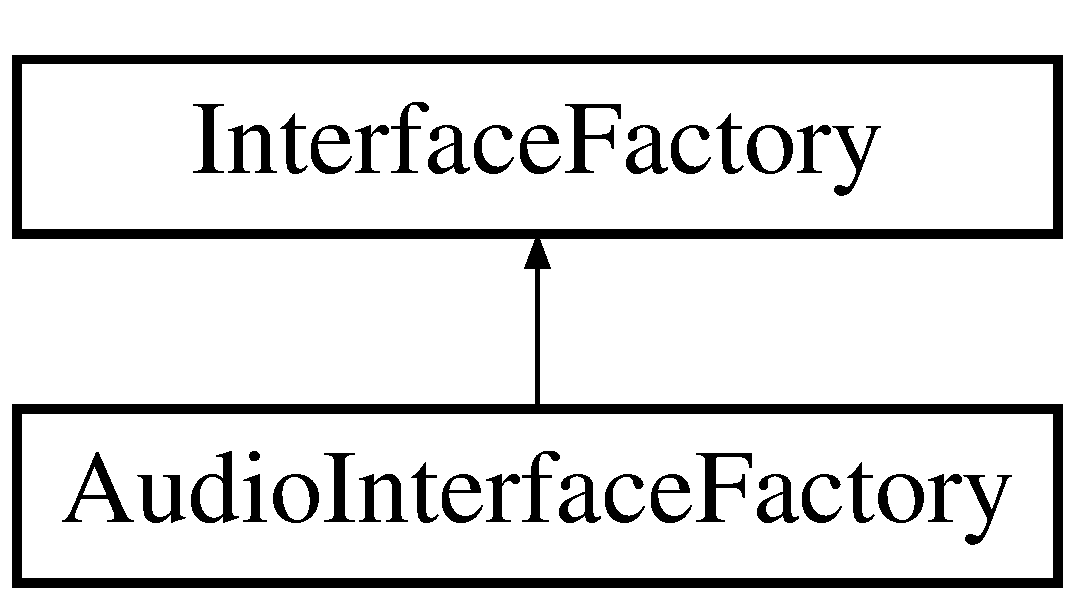
\includegraphics[height=2.000000cm]{classAudioInterfaceFactory}
\end{center}
\end{figure}
\subsection*{Fonctions membres publiques}
\begin{DoxyCompactItemize}
\item 
\hyperlink{classInterface}{Interface} \hyperlink{classAudioInterfaceFactory_ad5367033861d4aadd1ad0b0f5fa1caeb}{create\+Interface} (\hyperlink{classButtons}{Buttons} $\ast$b, \hyperlink{classFormat}{Format} $\ast$f)
\begin{DoxyCompactList}\small\item\em Crée l'interface adéquate à la lecture d'un fichier audio. \end{DoxyCompactList}\end{DoxyCompactItemize}


\subsection{Description détaillée}


Définition à la ligne 17 du fichier audio\+Interface\+Factory.\+hpp.



\subsection{Documentation des fonctions membres}
\hypertarget{classAudioInterfaceFactory_ad5367033861d4aadd1ad0b0f5fa1caeb}{\index{Audio\+Interface\+Factory@{Audio\+Interface\+Factory}!create\+Interface@{create\+Interface}}
\index{create\+Interface@{create\+Interface}!Audio\+Interface\+Factory@{Audio\+Interface\+Factory}}
\subsubsection[{create\+Interface}]{\setlength{\rightskip}{0pt plus 5cm}{\bf Interface} Audio\+Interface\+Factory\+::create\+Interface (
\begin{DoxyParamCaption}
\item[{{\bf Buttons} $\ast$}]{b, }
\item[{{\bf Format} $\ast$}]{f}
\end{DoxyParamCaption}
)\hspace{0.3cm}{\ttfamily [virtual]}}}\label{classAudioInterfaceFactory_ad5367033861d4aadd1ad0b0f5fa1caeb}


Crée l'interface adéquate à la lecture d'un fichier audio. 


\begin{DoxyParams}{Paramètres}
{\em \hyperlink{classButtonsVA}{Buttons\+V\+A}} & bva, \hyperlink{classFormatSmall}{Format\+Small} fs \\
\hline
\end{DoxyParams}
\begin{DoxyReturn}{Renvoie}
\hyperlink{classInterface}{Interface} audio 
\end{DoxyReturn}


Implémente \hyperlink{classInterfaceFactory}{Interface\+Factory}.



La documentation de cette classe a été générée à partir du fichier suivant \+:\begin{DoxyCompactItemize}
\item 
src/\+Abstract\+Factory/\hyperlink{audioInterfaceFactory_8hpp}{audio\+Interface\+Factory.\+hpp}\end{DoxyCompactItemize}

\hypertarget{classButtons}{\section{Référence de la classe Buttons}
\label{classButtons}\index{Buttons@{Buttons}}
}
Graphe d'héritage de Buttons\+:\begin{figure}[H]
\begin{center}
\leavevmode
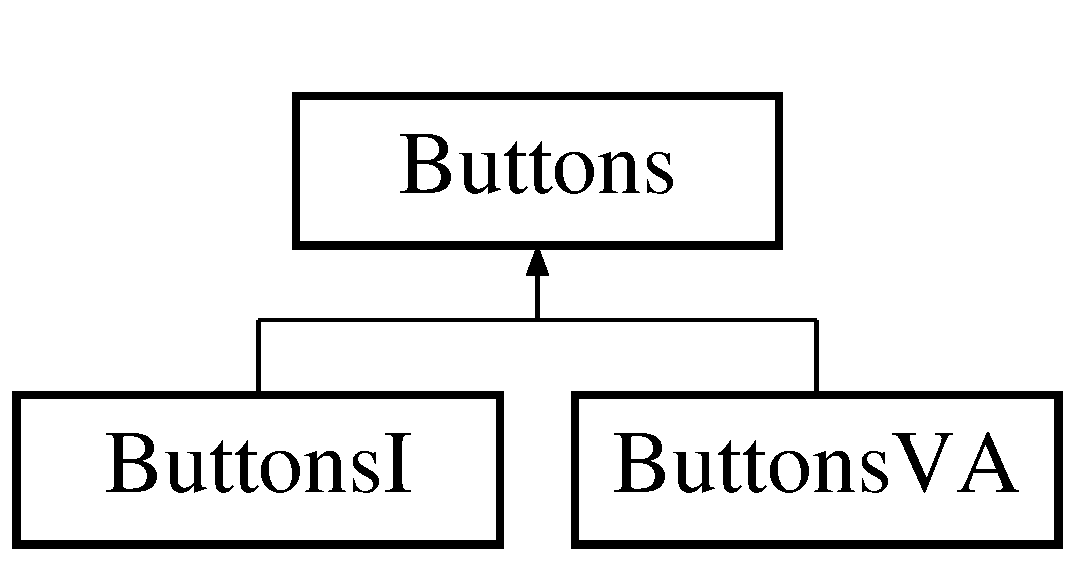
\includegraphics[height=2.000000cm]{classButtons}
\end{center}
\end{figure}
\subsection*{Fonctions membres publiques}
\begin{DoxyCompactItemize}
\item 
virtual void \hyperlink{classButtons_a785133d78116a4455166af0419f8283c}{create\+Buttons} (tgui\+::\+Gui $\ast$gui)=0
\begin{DoxyCompactList}\small\item\em Crée les boutons adéquats selon le type de média. \end{DoxyCompactList}\item 
virtual tgui\+::\+Button\+::\+Ptr \hyperlink{classButtons_a12154e1ff630b800dd9d5193e97202a0}{get\+Button\+N\+I} ()=0
\begin{DoxyCompactList}\small\item\em Accesseur virtuel. \end{DoxyCompactList}\item 
virtual tgui\+::\+Button\+::\+Ptr \hyperlink{classButtons_a82e85c87c04ead2f4bfbe661787e8094}{get\+Button\+P\+I} ()=0
\begin{DoxyCompactList}\small\item\em Accesseur virtuel. \end{DoxyCompactList}\item 
virtual tgui\+::\+Button\+::\+Ptr \hyperlink{classButtons_aea3bd52fcd2c6b41d71a02fb923be3c7}{get\+Button\+Pl} ()=0
\begin{DoxyCompactList}\small\item\em Accesseur virtuel. \end{DoxyCompactList}\item 
virtual tgui\+::\+Button\+::\+Ptr \hyperlink{classButtons_ab1fa18621507e31f3c6a66aaac91d065}{get\+Button\+Pa} ()=0
\begin{DoxyCompactList}\small\item\em Accesseur virtuel. \end{DoxyCompactList}\item 
virtual tgui\+::\+Button\+::\+Ptr \hyperlink{classButtons_a2e03184bee5b70e8acb1f53c98632350}{get\+Button\+St} ()=0
\begin{DoxyCompactList}\small\item\em Accesseur virtuel. \end{DoxyCompactList}\end{DoxyCompactItemize}


\subsection{Description détaillée}


Définition à la ligne 14 du fichier buttons.\+hpp.



\subsection{Documentation des fonctions membres}
\hypertarget{classButtons_a785133d78116a4455166af0419f8283c}{\index{Buttons@{Buttons}!create\+Buttons@{create\+Buttons}}
\index{create\+Buttons@{create\+Buttons}!Buttons@{Buttons}}
\subsubsection[{create\+Buttons}]{\setlength{\rightskip}{0pt plus 5cm}virtual void Buttons\+::create\+Buttons (
\begin{DoxyParamCaption}
\item[{tgui\+::\+Gui $\ast$}]{gui}
\end{DoxyParamCaption}
)\hspace{0.3cm}{\ttfamily [pure virtual]}}}\label{classButtons_a785133d78116a4455166af0419f8283c}


Crée les boutons adéquats selon le type de média. 

\begin{DoxyReturn}{Renvoie}
Un vecteur de boutons 
\end{DoxyReturn}


Implémenté dans \hyperlink{classButtonsVA_a2287bb2ca11365003534bda3c464d09f}{Buttons\+V\+A}, et \hyperlink{classButtonsI_ae79aa6a17f1251f34bffa009fcc0a2cd}{Buttons\+I}.

\hypertarget{classButtons_a12154e1ff630b800dd9d5193e97202a0}{\index{Buttons@{Buttons}!get\+Button\+N\+I@{get\+Button\+N\+I}}
\index{get\+Button\+N\+I@{get\+Button\+N\+I}!Buttons@{Buttons}}
\subsubsection[{get\+Button\+N\+I}]{\setlength{\rightskip}{0pt plus 5cm}virtual tgui\+::\+Button\+::\+Ptr Buttons\+::get\+Button\+N\+I (
\begin{DoxyParamCaption}
{}
\end{DoxyParamCaption}
)\hspace{0.3cm}{\ttfamily [pure virtual]}}}\label{classButtons_a12154e1ff630b800dd9d5193e97202a0}


Accesseur virtuel. 

\begin{DoxyReturn}{Renvoie}
\+\_\+bni, le Boutton\+N\+I (next image). 
\end{DoxyReturn}


Implémenté dans \hyperlink{classButtonsVA_a15145a6402d6a4688a9c50a5c4fae630}{Buttons\+V\+A}, et \hyperlink{classButtonsI_aecda6d6e3e44514421942ebe655eed79}{Buttons\+I}.

\hypertarget{classButtons_ab1fa18621507e31f3c6a66aaac91d065}{\index{Buttons@{Buttons}!get\+Button\+Pa@{get\+Button\+Pa}}
\index{get\+Button\+Pa@{get\+Button\+Pa}!Buttons@{Buttons}}
\subsubsection[{get\+Button\+Pa}]{\setlength{\rightskip}{0pt plus 5cm}virtual tgui\+::\+Button\+::\+Ptr Buttons\+::get\+Button\+Pa (
\begin{DoxyParamCaption}
{}
\end{DoxyParamCaption}
)\hspace{0.3cm}{\ttfamily [pure virtual]}}}\label{classButtons_ab1fa18621507e31f3c6a66aaac91d065}


Accesseur virtuel. 

\begin{DoxyReturn}{Renvoie}
\+\_\+bpa, le Boutton\+Pa (stop) 
\end{DoxyReturn}


Implémenté dans \hyperlink{classButtonsI_a312da091b65cf79a9963590af5076d18}{Buttons\+I}, et \hyperlink{classButtonsVA_ab222321660bfaed75d89645fa0ac37a0}{Buttons\+V\+A}.

\hypertarget{classButtons_a82e85c87c04ead2f4bfbe661787e8094}{\index{Buttons@{Buttons}!get\+Button\+P\+I@{get\+Button\+P\+I}}
\index{get\+Button\+P\+I@{get\+Button\+P\+I}!Buttons@{Buttons}}
\subsubsection[{get\+Button\+P\+I}]{\setlength{\rightskip}{0pt plus 5cm}virtual tgui\+::\+Button\+::\+Ptr Buttons\+::get\+Button\+P\+I (
\begin{DoxyParamCaption}
{}
\end{DoxyParamCaption}
)\hspace{0.3cm}{\ttfamily [pure virtual]}}}\label{classButtons_a82e85c87c04ead2f4bfbe661787e8094}


Accesseur virtuel. 

\begin{DoxyReturn}{Renvoie}
\+\_\+bpi, le Boutton\+P\+I (previous image). 
\end{DoxyReturn}


Implémenté dans \hyperlink{classButtonsVA_a625dec1c4ede8100580e957ddac22a17}{Buttons\+V\+A}, et \hyperlink{classButtonsI_a0d59693afaa2c3c01952b37dc42aeb0d}{Buttons\+I}.

\hypertarget{classButtons_aea3bd52fcd2c6b41d71a02fb923be3c7}{\index{Buttons@{Buttons}!get\+Button\+Pl@{get\+Button\+Pl}}
\index{get\+Button\+Pl@{get\+Button\+Pl}!Buttons@{Buttons}}
\subsubsection[{get\+Button\+Pl}]{\setlength{\rightskip}{0pt plus 5cm}virtual tgui\+::\+Button\+::\+Ptr Buttons\+::get\+Button\+Pl (
\begin{DoxyParamCaption}
{}
\end{DoxyParamCaption}
)\hspace{0.3cm}{\ttfamily [pure virtual]}}}\label{classButtons_aea3bd52fcd2c6b41d71a02fb923be3c7}


Accesseur virtuel. 

\begin{DoxyReturn}{Renvoie}
\+\_\+bpl, le Boutton\+Pl (play) 
\end{DoxyReturn}


Implémenté dans \hyperlink{classButtonsI_a77f7974ed70abfc6fbfc601a15ef1b61}{Buttons\+I}, et \hyperlink{classButtonsVA_a7c7a96011dc82bc8b57d0b84692ea52b}{Buttons\+V\+A}.

\hypertarget{classButtons_a2e03184bee5b70e8acb1f53c98632350}{\index{Buttons@{Buttons}!get\+Button\+St@{get\+Button\+St}}
\index{get\+Button\+St@{get\+Button\+St}!Buttons@{Buttons}}
\subsubsection[{get\+Button\+St}]{\setlength{\rightskip}{0pt plus 5cm}virtual tgui\+::\+Button\+::\+Ptr Buttons\+::get\+Button\+St (
\begin{DoxyParamCaption}
{}
\end{DoxyParamCaption}
)\hspace{0.3cm}{\ttfamily [pure virtual]}}}\label{classButtons_a2e03184bee5b70e8acb1f53c98632350}


Accesseur virtuel. 

\begin{DoxyReturn}{Renvoie}
\+\_\+bst, le Boutton\+St (pause) 
\end{DoxyReturn}


Implémenté dans \hyperlink{classButtonsI_a66e442c75b0110fdd73be6c7d8ea7b19}{Buttons\+I}, et \hyperlink{classButtonsVA_aad5dc82aec106cb00f78c92110daad0c}{Buttons\+V\+A}.



La documentation de cette classe a été générée à partir du fichier suivant \+:\begin{DoxyCompactItemize}
\item 
src/\+Abstract\+Factory/\hyperlink{buttons_8hpp}{buttons.\+hpp}\end{DoxyCompactItemize}

\hypertarget{classButtonsI}{\section{Référence de la classe Buttons\+I}
\label{classButtonsI}\index{Buttons\+I@{Buttons\+I}}
}
Graphe d'héritage de Buttons\+I\+:\begin{figure}[H]
\begin{center}
\leavevmode
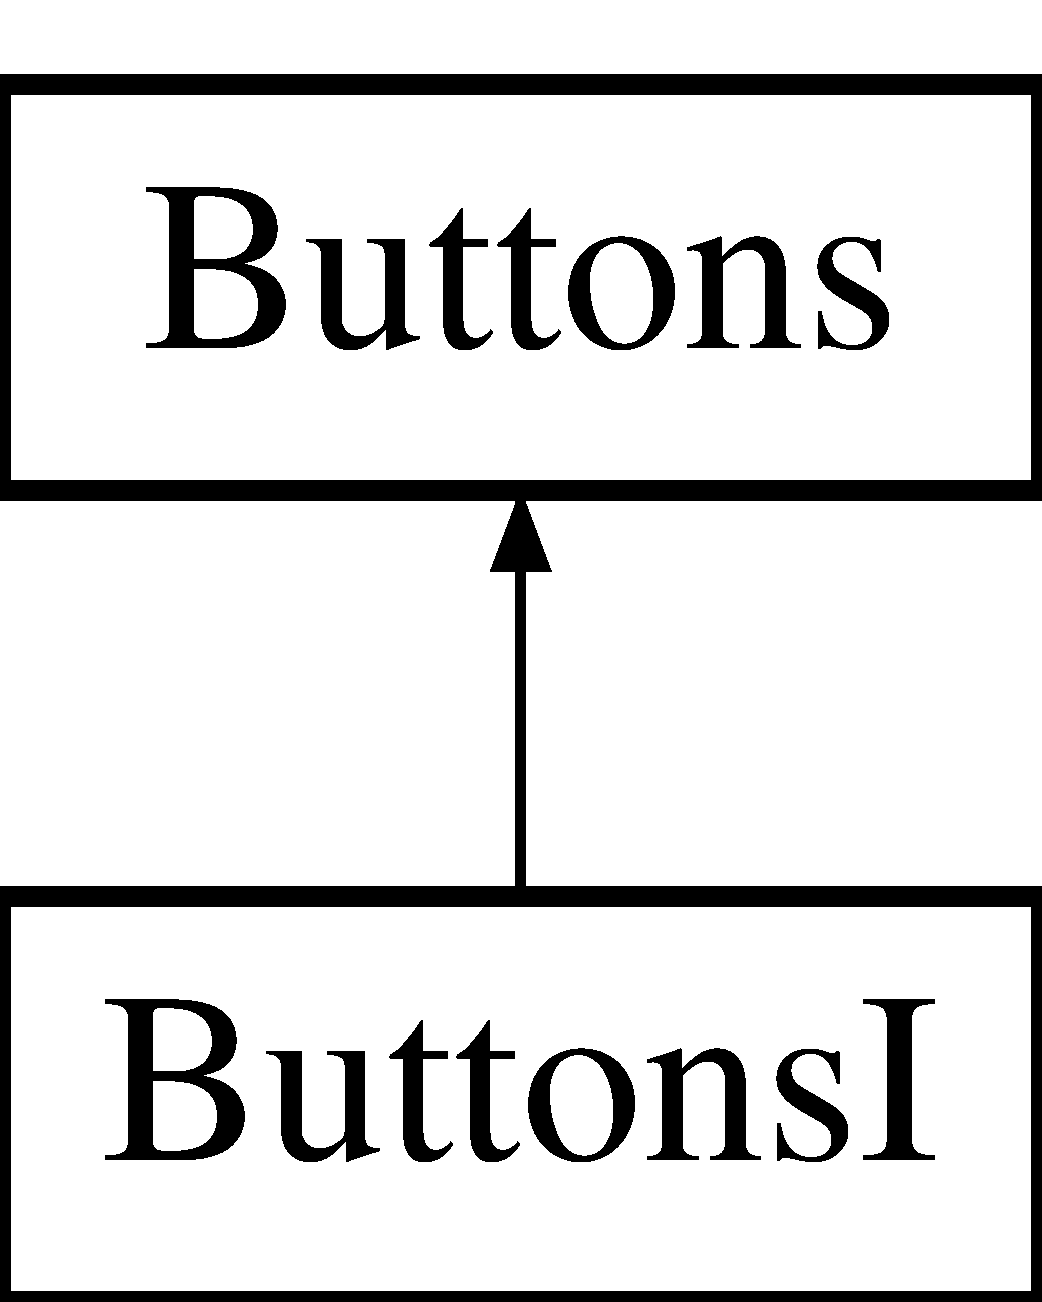
\includegraphics[height=2.000000cm]{classButtonsI}
\end{center}
\end{figure}
\subsection*{Fonctions membres publiques}
\begin{DoxyCompactItemize}
\item 
\hypertarget{classButtonsI_add8708005f41ef4fac952c8a82dda809}{{\bfseries Buttons\+I} (tgui\+::\+Button\+::\+Ptr bni, tgui\+::\+Button\+::\+Ptr bpi)}\label{classButtonsI_add8708005f41ef4fac952c8a82dda809}

\item 
\hypertarget{classButtonsI_aecda6d6e3e44514421942ebe655eed79}{tgui\+::\+Button\+::\+Ptr {\bfseries get\+Button\+N\+I} ()}\label{classButtonsI_aecda6d6e3e44514421942ebe655eed79}

\item 
\hypertarget{classButtonsI_a0d59693afaa2c3c01952b37dc42aeb0d}{tgui\+::\+Button\+::\+Ptr {\bfseries get\+Button\+P\+I} ()}\label{classButtonsI_a0d59693afaa2c3c01952b37dc42aeb0d}

\item 
\hypertarget{classButtonsI_a77f7974ed70abfc6fbfc601a15ef1b61}{tgui\+::\+Button\+::\+Ptr {\bfseries get\+Button\+Pl} ()}\label{classButtonsI_a77f7974ed70abfc6fbfc601a15ef1b61}

\item 
\hypertarget{classButtonsI_a312da091b65cf79a9963590af5076d18}{tgui\+::\+Button\+::\+Ptr {\bfseries get\+Button\+Pa} ()}\label{classButtonsI_a312da091b65cf79a9963590af5076d18}

\item 
\hypertarget{classButtonsI_a66e442c75b0110fdd73be6c7d8ea7b19}{tgui\+::\+Button\+::\+Ptr {\bfseries get\+Button\+St} ()}\label{classButtonsI_a66e442c75b0110fdd73be6c7d8ea7b19}

\item 
\hypertarget{classButtonsI_ae79aa6a17f1251f34bffa009fcc0a2cd}{void {\bfseries create\+Buttons} (tgui\+::\+Gui $\ast$gui)}\label{classButtonsI_ae79aa6a17f1251f34bffa009fcc0a2cd}

\end{DoxyCompactItemize}


\subsection{Description détaillée}


Définition à la ligne 16 du fichier buttons\+I.\+hpp.



La documentation de cette classe a été générée à partir du fichier suivant \+:\begin{DoxyCompactItemize}
\item 
src/\+Abstract\+Factory/\hyperlink{buttonsI_8hpp}{buttons\+I.\+hpp}\end{DoxyCompactItemize}

\hypertarget{classButtonsVA}{\section{Référence de la classe Buttons\+V\+A}
\label{classButtonsVA}\index{Buttons\+V\+A@{Buttons\+V\+A}}
}
Graphe d'héritage de Buttons\+V\+A\+:\begin{figure}[H]
\begin{center}
\leavevmode
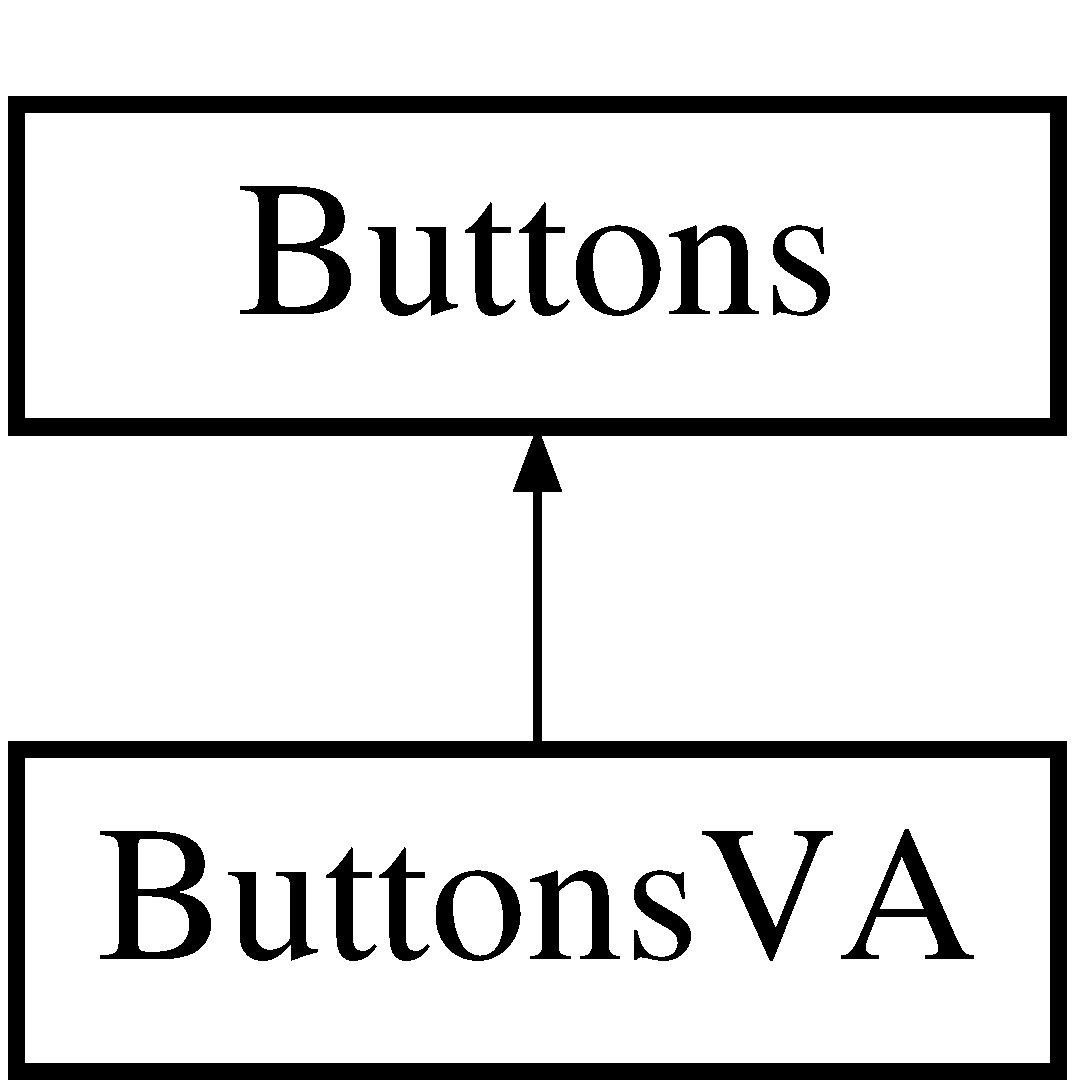
\includegraphics[height=2.000000cm]{classButtonsVA}
\end{center}
\end{figure}
\subsection*{Fonctions membres publiques}
\begin{DoxyCompactItemize}
\item 
\hypertarget{classButtonsVA_a146e69faf1e042093a69c2800b35c55b}{{\bfseries Buttons\+V\+A} (tgui\+::\+Button\+::\+Ptr bpl, tgui\+::\+Button\+::\+Ptr bpa, tgui\+::\+Button\+::\+Ptr bst)}\label{classButtonsVA_a146e69faf1e042093a69c2800b35c55b}

\item 
\hypertarget{classButtonsVA_a7c7a96011dc82bc8b57d0b84692ea52b}{tgui\+::\+Button\+::\+Ptr {\bfseries get\+Button\+Pl} ()}\label{classButtonsVA_a7c7a96011dc82bc8b57d0b84692ea52b}

\item 
\hypertarget{classButtonsVA_ab222321660bfaed75d89645fa0ac37a0}{tgui\+::\+Button\+::\+Ptr {\bfseries get\+Button\+Pa} ()}\label{classButtonsVA_ab222321660bfaed75d89645fa0ac37a0}

\item 
\hypertarget{classButtonsVA_aad5dc82aec106cb00f78c92110daad0c}{tgui\+::\+Button\+::\+Ptr {\bfseries get\+Button\+St} ()}\label{classButtonsVA_aad5dc82aec106cb00f78c92110daad0c}

\item 
\hypertarget{classButtonsVA_a625dec1c4ede8100580e957ddac22a17}{tgui\+::\+Button\+::\+Ptr {\bfseries get\+Button\+P\+I} ()}\label{classButtonsVA_a625dec1c4ede8100580e957ddac22a17}

\item 
\hypertarget{classButtonsVA_a15145a6402d6a4688a9c50a5c4fae630}{tgui\+::\+Button\+::\+Ptr {\bfseries get\+Button\+N\+I} ()}\label{classButtonsVA_a15145a6402d6a4688a9c50a5c4fae630}

\item 
\hypertarget{classButtonsVA_a2287bb2ca11365003534bda3c464d09f}{void {\bfseries create\+Buttons} (tgui\+::\+Gui $\ast$gui)}\label{classButtonsVA_a2287bb2ca11365003534bda3c464d09f}

\end{DoxyCompactItemize}


\subsection{Description détaillée}


Définition à la ligne 16 du fichier buttons\+V\+A.\+hpp.



La documentation de cette classe a été générée à partir du fichier suivant \+:\begin{DoxyCompactItemize}
\item 
src/\+Abstract\+Factory/\hyperlink{buttonsVA_8hpp}{buttons\+V\+A.\+hpp}\end{DoxyCompactItemize}

\hypertarget{classDir}{\section{Référence de la classe Dir}
\label{classDir}\index{Dir@{Dir}}
}
\subsection*{Fonctions membres publiques}
\begin{DoxyCompactItemize}
\item 
\hypertarget{classDir_af635ae8d3f73e276fd4809443294c922}{void {\bfseries set\+Files\+Vector} (std\+::string path)}\label{classDir_af635ae8d3f73e276fd4809443294c922}

\item 
\hypertarget{classDir_a93214e588267bd1b9fea42ab5334477e}{std\+::vector$<$ std\+::string $>$ {\bfseries get\+Files\+Vector} ()}\label{classDir_a93214e588267bd1b9fea42ab5334477e}

\item 
\hypertarget{classDir_a8a201475486c0a0e7a8d8243e6b50df2}{void {\bfseries create\+Dir\+Widget} (tgui\+::\+Gui $\ast$gui)}\label{classDir_a8a201475486c0a0e7a8d8243e6b50df2}

\item 
\hypertarget{classDir_a86b006137e1060d5219ca36da54c57b6}{std\+::string {\bfseries return\+Path} (int id)}\label{classDir_a86b006137e1060d5219ca36da54c57b6}

\item 
\hypertarget{classDir_aab53eceedc1485700282493f41fa9227}{int {\bfseries get\+Item\+Selected} ()}\label{classDir_aab53eceedc1485700282493f41fa9227}

\item 
\hypertarget{classDir_abde90c9dd3b727623700c6564b6c501b}{void {\bfseries set\+Selected\+Item} (int i)}\label{classDir_abde90c9dd3b727623700c6564b6c501b}

\item 
\hypertarget{classDir_aedeb46b9ae54b81a712a53efa3144c8c}{void {\bfseries hide} ()}\label{classDir_aedeb46b9ae54b81a712a53efa3144c8c}

\item 
\hypertarget{classDir_a2fe90aa7cdf0e3fdc9cd46785d191e6f}{std\+::string {\bfseries get\+Item} (int i)}\label{classDir_a2fe90aa7cdf0e3fdc9cd46785d191e6f}

\end{DoxyCompactItemize}


\subsection{Description détaillée}


Définition à la ligne 17 du fichier Dir.\+hpp.



La documentation de cette classe a été générée à partir du fichier suivant \+:\begin{DoxyCompactItemize}
\item 
src/\+Dir/\hyperlink{Dir_8hpp}{Dir.\+hpp}\end{DoxyCompactItemize}

\hypertarget{classEtatA}{\section{Référence de la classe Etat\+A}
\label{classEtatA}\index{Etat\+A@{Etat\+A}}
}
Graphe d'héritage de Etat\+A\+:\begin{figure}[H]
\begin{center}
\leavevmode
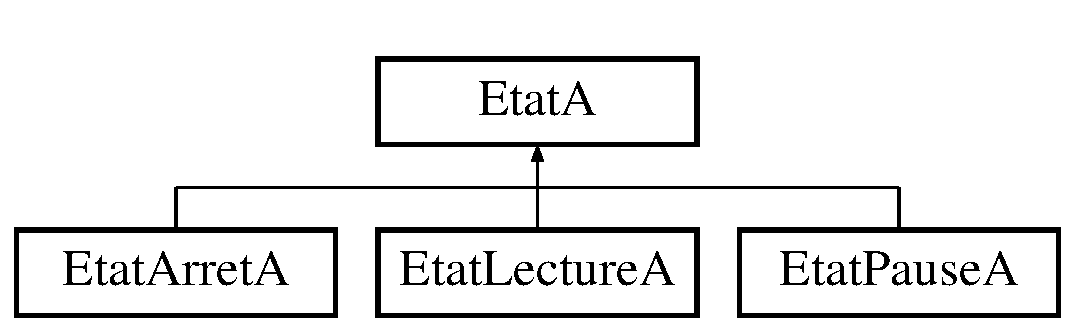
\includegraphics[height=2.000000cm]{classEtatA}
\end{center}
\end{figure}
\subsection*{Fonctions membres publiques}
\begin{DoxyCompactItemize}
\item 
\hypertarget{classEtatA_a8e1a9dfd3470c1230c28b3e326330f4c}{virtual void \hyperlink{classEtatA_a8e1a9dfd3470c1230c28b3e326330f4c}{utiliser\+Bouton\+Stop\+A} (sf\+::\+Sound $\ast$sound)}\label{classEtatA_a8e1a9dfd3470c1230c28b3e326330f4c}

\begin{DoxyCompactList}\small\item\em utiliser\+Bouton\+Stop\+A \+: selon l'etat, effectue l'action du bouttonstop. Virtuel \end{DoxyCompactList}\item 
\hypertarget{classEtatA_aa3a201e53fafd92629cbd9634a037c8e}{virtual void \hyperlink{classEtatA_aa3a201e53fafd92629cbd9634a037c8e}{utiliser\+Bouton\+Pause\+A} (sf\+::\+Sound $\ast$sound)}\label{classEtatA_aa3a201e53fafd92629cbd9634a037c8e}

\begin{DoxyCompactList}\small\item\em utiliser\+Bouton\+Pause\+A \+: selon l'etat, effectue l'action du bouttonpause. Virtuel \end{DoxyCompactList}\item 
\hypertarget{classEtatA_a268ddc5db2a85a859d3d81a897bd47c8}{virtual void \hyperlink{classEtatA_a268ddc5db2a85a859d3d81a897bd47c8}{utiliser\+Bouton\+Lecture\+A} (sf\+::\+Sound $\ast$sound)}\label{classEtatA_a268ddc5db2a85a859d3d81a897bd47c8}

\begin{DoxyCompactList}\small\item\em utiliser\+Bouton\+Lecture\+A \+: selon l'etat, effectue l'action du bouttonlecture. Virtuel \end{DoxyCompactList}\item 
\hypertarget{classEtatA_abd2d754e4d12f3fbbd5b9cf06bfe1a21}{virtual void \hyperlink{classEtatA_abd2d754e4d12f3fbbd5b9cf06bfe1a21}{afficher\+A} ()=0}\label{classEtatA_abd2d754e4d12f3fbbd5b9cf06bfe1a21}

\begin{DoxyCompactList}\small\item\em afficher\+A \+: selon l'etat, affiche l'état de l'audio. Virtuel \end{DoxyCompactList}\end{DoxyCompactItemize}


\subsection{Description détaillée}


Définition à la ligne 15 du fichier etat\+A.\+hpp.



La documentation de cette classe a été générée à partir du fichier suivant \+:\begin{DoxyCompactItemize}
\item 
src/\+State\+Audio/\hyperlink{etatA_8hpp}{etat\+A.\+hpp}\end{DoxyCompactItemize}

\hypertarget{classEtatArretA}{\section{Référence de la classe Etat\+Arret\+A}
\label{classEtatArretA}\index{Etat\+Arret\+A@{Etat\+Arret\+A}}
}
Graphe d'héritage de Etat\+Arret\+A\+:\begin{figure}[H]
\begin{center}
\leavevmode
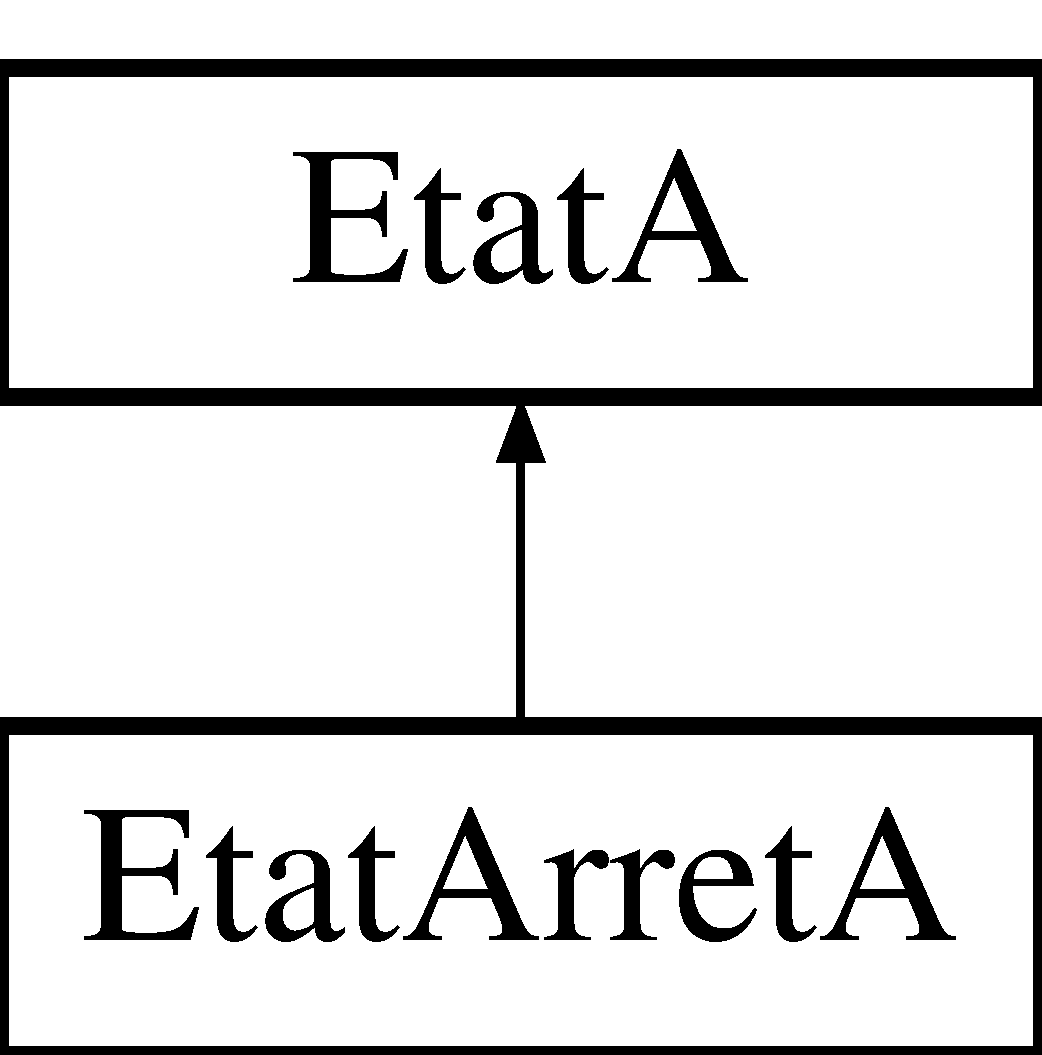
\includegraphics[height=2.000000cm]{classEtatArretA}
\end{center}
\end{figure}
\subsection*{Fonctions membres publiques}
\begin{DoxyCompactItemize}
\item 
\hypertarget{classEtatArretA_a283a80478fd920238ba7152d0cdfea5c}{\hyperlink{classEtatArretA_a283a80478fd920238ba7152d0cdfea5c}{Etat\+Arret\+A} ()}\label{classEtatArretA_a283a80478fd920238ba7152d0cdfea5c}

\begin{DoxyCompactList}\small\item\em Constructeur. \end{DoxyCompactList}\item 
\hyperlink{classEtatArretA_aa5235b55db8f80efd91b2ee3bbd842de}{Etat\+Arret\+A} (\hyperlink{classAudio}{Audio} $\ast$a)
\begin{DoxyCompactList}\small\item\em Constructeur. \end{DoxyCompactList}\item 
\hypertarget{classEtatArretA_a56aef7900e5a00efc1915b263522fffd}{void \hyperlink{classEtatArretA_a56aef7900e5a00efc1915b263522fffd}{utiliser\+Bouton\+Lecture\+A} (sf\+::\+Sound $\ast$sound)}\label{classEtatArretA_a56aef7900e5a00efc1915b263522fffd}

\begin{DoxyCompactList}\small\item\em utiliser\+Bouton\+Lecture\+A \+: passe l'audio dans l'état lecture \end{DoxyCompactList}\item 
\hypertarget{classEtatArretA_a44b510722d620d74ed69b7bba4208558}{void \hyperlink{classEtatArretA_a44b510722d620d74ed69b7bba4208558}{afficher\+A} ()}\label{classEtatArretA_a44b510722d620d74ed69b7bba4208558}

\begin{DoxyCompactList}\small\item\em afficher\+A \+: afficher l'état arret \end{DoxyCompactList}\end{DoxyCompactItemize}


\subsection{Description détaillée}


Définition à la ligne 14 du fichier etat\+Arret\+A.\+hpp.



\subsection{Documentation des constructeurs et destructeur}
\hypertarget{classEtatArretA_aa5235b55db8f80efd91b2ee3bbd842de}{\index{Etat\+Arret\+A@{Etat\+Arret\+A}!Etat\+Arret\+A@{Etat\+Arret\+A}}
\index{Etat\+Arret\+A@{Etat\+Arret\+A}!Etat\+Arret\+A@{Etat\+Arret\+A}}
\subsubsection[{Etat\+Arret\+A}]{\setlength{\rightskip}{0pt plus 5cm}Etat\+Arret\+A\+::\+Etat\+Arret\+A (
\begin{DoxyParamCaption}
\item[{{\bf Audio} $\ast$}]{a}
\end{DoxyParamCaption}
)}}\label{classEtatArretA_aa5235b55db8f80efd91b2ee3bbd842de}


Constructeur. 


\begin{DoxyParams}{Paramètres}
{\em Audio$\ast$} & a \+: pointeur vers audio \\
\hline
\end{DoxyParams}


La documentation de cette classe a été générée à partir du fichier suivant \+:\begin{DoxyCompactItemize}
\item 
src/\+State\+Audio/\hyperlink{etatArretA_8hpp}{etat\+Arret\+A.\+hpp}\end{DoxyCompactItemize}

\hypertarget{classEtatArretV}{\section{Référence de la classe Etat\+Arret\+V}
\label{classEtatArretV}\index{Etat\+Arret\+V@{Etat\+Arret\+V}}
}
Graphe d'héritage de Etat\+Arret\+V\+:\begin{figure}[H]
\begin{center}
\leavevmode
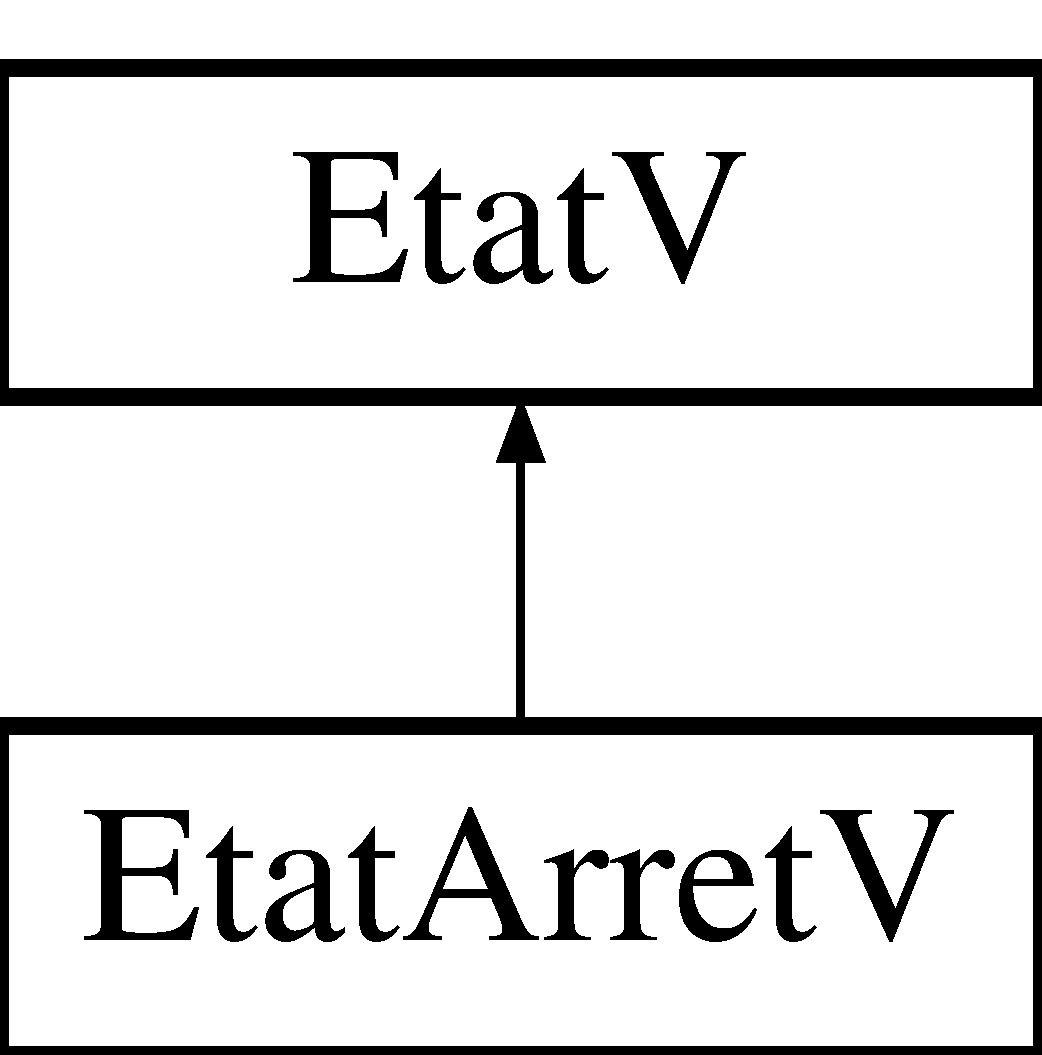
\includegraphics[height=2.000000cm]{classEtatArretV}
\end{center}
\end{figure}
\subsection*{Fonctions membres publiques}
\begin{DoxyCompactItemize}
\item 
\hypertarget{classEtatArretV_a5acc53409e45b619e4a4787822380813}{\hyperlink{classEtatArretV_a5acc53409e45b619e4a4787822380813}{Etat\+Arret\+V} ()}\label{classEtatArretV_a5acc53409e45b619e4a4787822380813}

\begin{DoxyCompactList}\small\item\em Constructeur. \end{DoxyCompactList}\item 
\hyperlink{classEtatArretV_ab5cd0f3379bab61653f42732b446c266}{Etat\+Arret\+V} (\hyperlink{classVideo}{Video} $\ast$v)
\begin{DoxyCompactList}\small\item\em Constructeur. \end{DoxyCompactList}\item 
\hypertarget{classEtatArretV_af74e3607e8f4a966139d12929ee29f23}{void \hyperlink{classEtatArretV_af74e3607e8f4a966139d12929ee29f23}{utiliser\+Bouton\+Lecture\+V} (sfe\+::\+Movie $\ast$movie)}\label{classEtatArretV_af74e3607e8f4a966139d12929ee29f23}

\begin{DoxyCompactList}\small\item\em utiliser\+Bouton\+Lecture\+V \+: passe la video dans l'état lecture \end{DoxyCompactList}\item 
\hypertarget{classEtatArretV_a87941d7ebc9647c7c7dd0d3e8c901a35}{void \hyperlink{classEtatArretV_a87941d7ebc9647c7c7dd0d3e8c901a35}{afficher\+V} ()}\label{classEtatArretV_a87941d7ebc9647c7c7dd0d3e8c901a35}

\begin{DoxyCompactList}\small\item\em afficher\+V \+: afficher l'état arret \end{DoxyCompactList}\end{DoxyCompactItemize}


\subsection{Description détaillée}


Définition à la ligne 13 du fichier etat\+Arret\+V.\+hpp.



\subsection{Documentation des constructeurs et destructeur}
\hypertarget{classEtatArretV_ab5cd0f3379bab61653f42732b446c266}{\index{Etat\+Arret\+V@{Etat\+Arret\+V}!Etat\+Arret\+V@{Etat\+Arret\+V}}
\index{Etat\+Arret\+V@{Etat\+Arret\+V}!Etat\+Arret\+V@{Etat\+Arret\+V}}
\subsubsection[{Etat\+Arret\+V}]{\setlength{\rightskip}{0pt plus 5cm}Etat\+Arret\+V\+::\+Etat\+Arret\+V (
\begin{DoxyParamCaption}
\item[{{\bf Video} $\ast$}]{v}
\end{DoxyParamCaption}
)}}\label{classEtatArretV_ab5cd0f3379bab61653f42732b446c266}


Constructeur. 


\begin{DoxyParams}{Paramètres}
{\em Video$\ast$} & v \+: pointeur vers video \\
\hline
\end{DoxyParams}


La documentation de cette classe a été générée à partir du fichier suivant \+:\begin{DoxyCompactItemize}
\item 
src/\+State\+Video/\hyperlink{etatArretV_8hpp}{etat\+Arret\+V.\+hpp}\end{DoxyCompactItemize}

\hypertarget{classEtatLectureA}{\section{Référence de la classe Etat\+Lecture\+A}
\label{classEtatLectureA}\index{Etat\+Lecture\+A@{Etat\+Lecture\+A}}
}
Graphe d'héritage de Etat\+Lecture\+A\+:\begin{figure}[H]
\begin{center}
\leavevmode
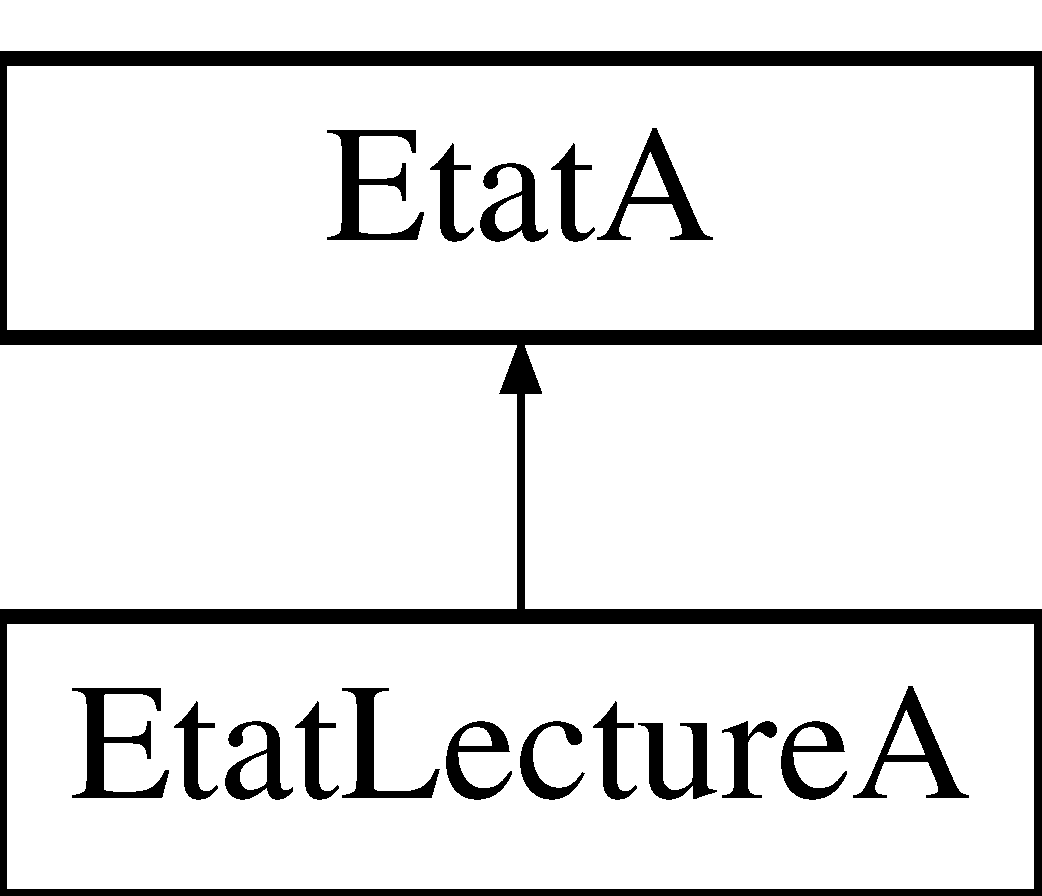
\includegraphics[height=2.000000cm]{classEtatLectureA}
\end{center}
\end{figure}
\subsection*{Fonctions membres publiques}
\begin{DoxyCompactItemize}
\item 
\hypertarget{classEtatLectureA_af296a1105e5b5ad7656b770e58d0b499}{\hyperlink{classEtatLectureA_af296a1105e5b5ad7656b770e58d0b499}{Etat\+Lecture\+A} ()}\label{classEtatLectureA_af296a1105e5b5ad7656b770e58d0b499}

\begin{DoxyCompactList}\small\item\em Constructeur. \end{DoxyCompactList}\item 
\hyperlink{classEtatLectureA_a184cb5df01065ea377e42d6c6167a248}{Etat\+Lecture\+A} (\hyperlink{classAudio}{Audio} $\ast$a)
\begin{DoxyCompactList}\small\item\em Constructeur. \end{DoxyCompactList}\item 
\hypertarget{classEtatLectureA_a6f25a0722b9913e2ed963f9d5e7c29c4}{void \hyperlink{classEtatLectureA_a6f25a0722b9913e2ed963f9d5e7c29c4}{utiliser\+Bouton\+Stop\+A} (sf\+::\+Sound $\ast$sound)}\label{classEtatLectureA_a6f25a0722b9913e2ed963f9d5e7c29c4}

\begin{DoxyCompactList}\small\item\em utiliser\+Bouton\+Stop\+A \+: passe l'audio dans l'état stop \end{DoxyCompactList}\item 
\hypertarget{classEtatLectureA_a079893f8566da8b9ef1bace9bc92aa8e}{void \hyperlink{classEtatLectureA_a079893f8566da8b9ef1bace9bc92aa8e}{utiliser\+Bouton\+Pause\+A} (sf\+::\+Sound $\ast$sound)}\label{classEtatLectureA_a079893f8566da8b9ef1bace9bc92aa8e}

\begin{DoxyCompactList}\small\item\em utiliser\+Bouton\+Pause\+A \+: passe l'audio dans l'état pause \end{DoxyCompactList}\item 
\hypertarget{classEtatLectureA_ad1ca4a4b0fa21d6bc1e51b04187cf63f}{void \hyperlink{classEtatLectureA_ad1ca4a4b0fa21d6bc1e51b04187cf63f}{afficher\+A} ()}\label{classEtatLectureA_ad1ca4a4b0fa21d6bc1e51b04187cf63f}

\begin{DoxyCompactList}\small\item\em afficher\+A \+: affiche l'état lecture \end{DoxyCompactList}\end{DoxyCompactItemize}


\subsection{Description détaillée}


Définition à la ligne 13 du fichier etat\+Lecture\+A.\+hpp.



\subsection{Documentation des constructeurs et destructeur}
\hypertarget{classEtatLectureA_a184cb5df01065ea377e42d6c6167a248}{\index{Etat\+Lecture\+A@{Etat\+Lecture\+A}!Etat\+Lecture\+A@{Etat\+Lecture\+A}}
\index{Etat\+Lecture\+A@{Etat\+Lecture\+A}!Etat\+Lecture\+A@{Etat\+Lecture\+A}}
\subsubsection[{Etat\+Lecture\+A}]{\setlength{\rightskip}{0pt plus 5cm}Etat\+Lecture\+A\+::\+Etat\+Lecture\+A (
\begin{DoxyParamCaption}
\item[{{\bf Audio} $\ast$}]{a}
\end{DoxyParamCaption}
)}}\label{classEtatLectureA_a184cb5df01065ea377e42d6c6167a248}


Constructeur. 


\begin{DoxyParams}{Paramètres}
{\em Audio$\ast$} & a \+: pointeur vers audio \\
\hline
\end{DoxyParams}


La documentation de cette classe a été générée à partir du fichier suivant \+:\begin{DoxyCompactItemize}
\item 
src/\+State\+Audio/\hyperlink{etatLectureA_8hpp}{etat\+Lecture\+A.\+hpp}\end{DoxyCompactItemize}

\hypertarget{classEtatLectureV}{\section{Référence de la classe Etat\+Lecture\+V}
\label{classEtatLectureV}\index{Etat\+Lecture\+V@{Etat\+Lecture\+V}}
}
Graphe d'héritage de Etat\+Lecture\+V\+:\begin{figure}[H]
\begin{center}
\leavevmode
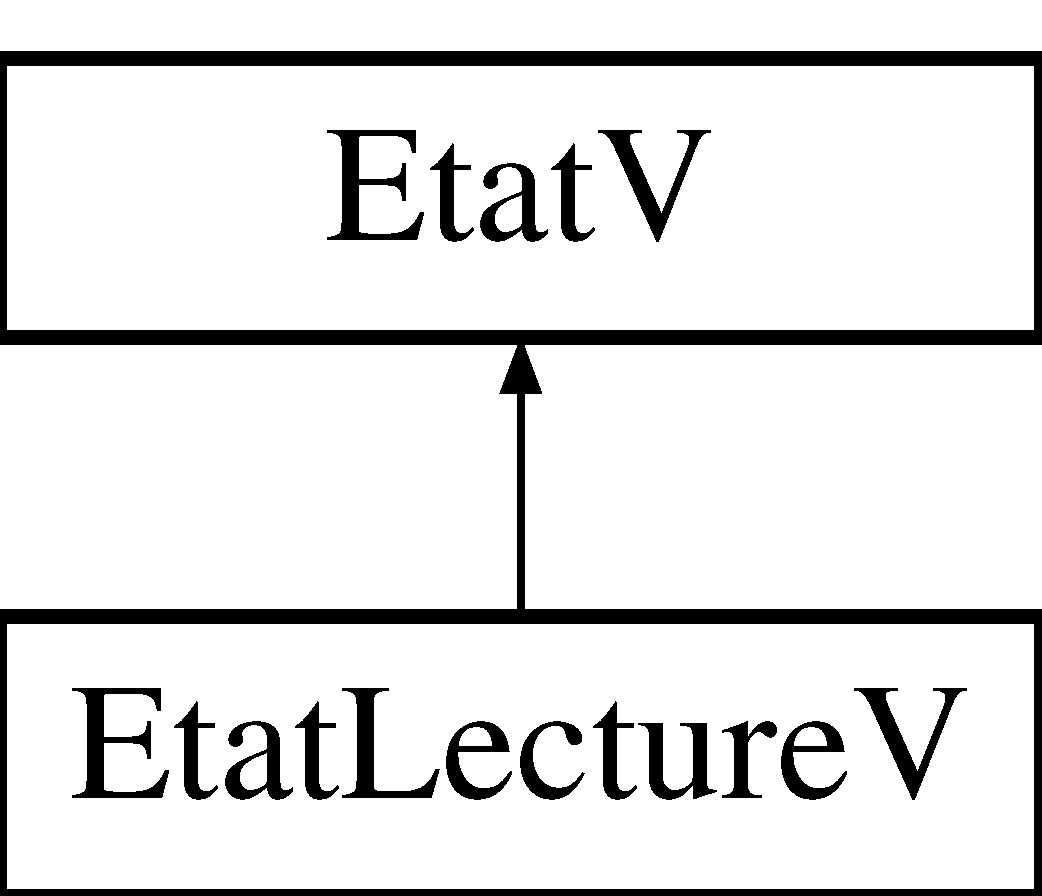
\includegraphics[height=2.000000cm]{classEtatLectureV}
\end{center}
\end{figure}
\subsection*{Fonctions membres publiques}
\begin{DoxyCompactItemize}
\item 
\hypertarget{classEtatLectureV_a3d1e649e72665157198fb438169c09d7}{\hyperlink{classEtatLectureV_a3d1e649e72665157198fb438169c09d7}{Etat\+Lecture\+V} ()}\label{classEtatLectureV_a3d1e649e72665157198fb438169c09d7}

\begin{DoxyCompactList}\small\item\em Constructeur. \end{DoxyCompactList}\item 
\hyperlink{classEtatLectureV_af053295ec024e0afd1a08dfd861ec9a0}{Etat\+Lecture\+V} (\hyperlink{classVideo}{Video} $\ast$a)
\begin{DoxyCompactList}\small\item\em Constructeur. \end{DoxyCompactList}\item 
\hypertarget{classEtatLectureV_a9204aecf5df3dccc8414a3afb547c325}{void \hyperlink{classEtatLectureV_a9204aecf5df3dccc8414a3afb547c325}{utiliser\+Bouton\+Stop\+V} (sfe\+::\+Movie $\ast$movie)}\label{classEtatLectureV_a9204aecf5df3dccc8414a3afb547c325}

\begin{DoxyCompactList}\small\item\em utiliser\+Bouton\+Stop\+V \+: passe la video dans l'état stop \end{DoxyCompactList}\item 
\hypertarget{classEtatLectureV_a1ac75124b057cd5ffa4ad7aca3981cf4}{void \hyperlink{classEtatLectureV_a1ac75124b057cd5ffa4ad7aca3981cf4}{utiliser\+Bouton\+Pause\+V} (sfe\+::\+Movie $\ast$movie)}\label{classEtatLectureV_a1ac75124b057cd5ffa4ad7aca3981cf4}

\begin{DoxyCompactList}\small\item\em utiliser\+Bouton\+Pause\+V \+: passe la video dans l'état pause \end{DoxyCompactList}\item 
\hypertarget{classEtatLectureV_aeb97541e60e26c71a7053ae30dd78029}{void \hyperlink{classEtatLectureV_aeb97541e60e26c71a7053ae30dd78029}{afficher\+V} ()}\label{classEtatLectureV_aeb97541e60e26c71a7053ae30dd78029}

\begin{DoxyCompactList}\small\item\em afficher\+V \+: affiche l'état lecture \end{DoxyCompactList}\end{DoxyCompactItemize}


\subsection{Description détaillée}


Définition à la ligne 13 du fichier etat\+Lecture\+V.\+hpp.



\subsection{Documentation des constructeurs et destructeur}
\hypertarget{classEtatLectureV_af053295ec024e0afd1a08dfd861ec9a0}{\index{Etat\+Lecture\+V@{Etat\+Lecture\+V}!Etat\+Lecture\+V@{Etat\+Lecture\+V}}
\index{Etat\+Lecture\+V@{Etat\+Lecture\+V}!Etat\+Lecture\+V@{Etat\+Lecture\+V}}
\subsubsection[{Etat\+Lecture\+V}]{\setlength{\rightskip}{0pt plus 5cm}Etat\+Lecture\+V\+::\+Etat\+Lecture\+V (
\begin{DoxyParamCaption}
\item[{{\bf Video} $\ast$}]{a}
\end{DoxyParamCaption}
)}}\label{classEtatLectureV_af053295ec024e0afd1a08dfd861ec9a0}


Constructeur. 


\begin{DoxyParams}{Paramètres}
{\em Video$\ast$} & a \+: pointeur vers video \\
\hline
\end{DoxyParams}


La documentation de cette classe a été générée à partir du fichier suivant \+:\begin{DoxyCompactItemize}
\item 
src/\+State\+Video/\hyperlink{etatLectureV_8hpp}{etat\+Lecture\+V.\+hpp}\end{DoxyCompactItemize}

\hypertarget{classEtatPauseA}{\section{Référence de la classe Etat\+Pause\+A}
\label{classEtatPauseA}\index{Etat\+Pause\+A@{Etat\+Pause\+A}}
}
Graphe d'héritage de Etat\+Pause\+A\+:\begin{figure}[H]
\begin{center}
\leavevmode
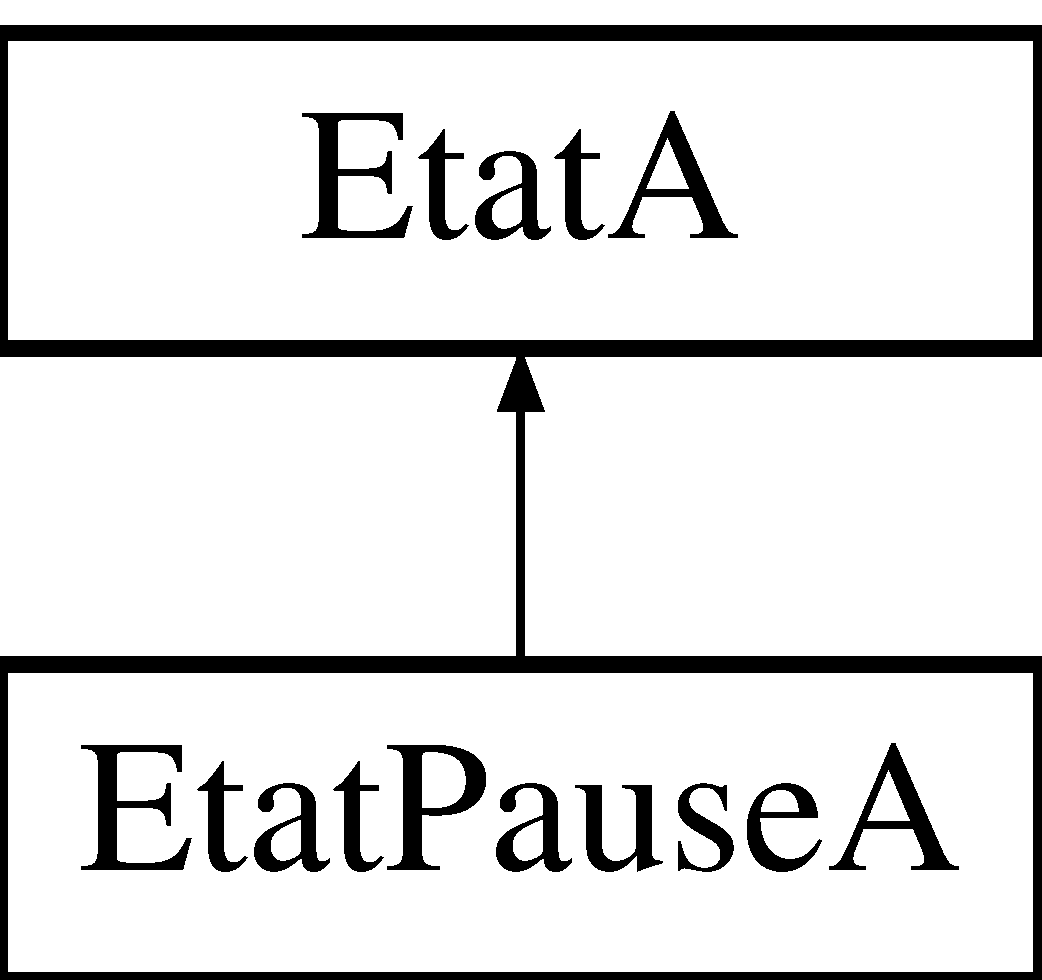
\includegraphics[height=2.000000cm]{classEtatPauseA}
\end{center}
\end{figure}
\subsection*{Fonctions membres publiques}
\begin{DoxyCompactItemize}
\item 
\hypertarget{classEtatPauseA_a2980943694ceb3f46af2ef813a9a2921}{\hyperlink{classEtatPauseA_a2980943694ceb3f46af2ef813a9a2921}{Etat\+Pause\+A} ()}\label{classEtatPauseA_a2980943694ceb3f46af2ef813a9a2921}

\begin{DoxyCompactList}\small\item\em Constructeur. \end{DoxyCompactList}\item 
\hyperlink{classEtatPauseA_a76a16c20d023e39e72022076c768350d}{Etat\+Pause\+A} (\hyperlink{classAudio}{Audio} $\ast$a)
\begin{DoxyCompactList}\small\item\em Constructeur. \end{DoxyCompactList}\item 
\hypertarget{classEtatPauseA_ae5b24db5e5dac2e537d15e8f06cb6031}{void \hyperlink{classEtatPauseA_ae5b24db5e5dac2e537d15e8f06cb6031}{utiliser\+Bouton\+Stop\+A} (sf\+::\+Sound $\ast$sound)}\label{classEtatPauseA_ae5b24db5e5dac2e537d15e8f06cb6031}

\begin{DoxyCompactList}\small\item\em utiliser\+Bouton\+Stop\+A \+: passe l'audio dans l'état stop \end{DoxyCompactList}\item 
\hypertarget{classEtatPauseA_ade87301319d07c8a39650d520420d1c0}{void \hyperlink{classEtatPauseA_ade87301319d07c8a39650d520420d1c0}{utiliser\+Bouton\+Lecture\+A} (sf\+::\+Sound $\ast$sound)}\label{classEtatPauseA_ade87301319d07c8a39650d520420d1c0}

\begin{DoxyCompactList}\small\item\em utiliser\+Bouton\+Lecture\+A \+: passe l'audio dans l'état lecture \end{DoxyCompactList}\item 
\hypertarget{classEtatPauseA_a0fc6595ed30426469fd65fb53f732a2c}{void \hyperlink{classEtatPauseA_a0fc6595ed30426469fd65fb53f732a2c}{afficher\+A} ()}\label{classEtatPauseA_a0fc6595ed30426469fd65fb53f732a2c}

\begin{DoxyCompactList}\small\item\em afficher\+A \+: affiche l'état pause \end{DoxyCompactList}\end{DoxyCompactItemize}


\subsection{Description détaillée}


Définition à la ligne 14 du fichier etat\+Pause\+A.\+hpp.



\subsection{Documentation des constructeurs et destructeur}
\hypertarget{classEtatPauseA_a76a16c20d023e39e72022076c768350d}{\index{Etat\+Pause\+A@{Etat\+Pause\+A}!Etat\+Pause\+A@{Etat\+Pause\+A}}
\index{Etat\+Pause\+A@{Etat\+Pause\+A}!Etat\+Pause\+A@{Etat\+Pause\+A}}
\subsubsection[{Etat\+Pause\+A}]{\setlength{\rightskip}{0pt plus 5cm}Etat\+Pause\+A\+::\+Etat\+Pause\+A (
\begin{DoxyParamCaption}
\item[{{\bf Audio} $\ast$}]{a}
\end{DoxyParamCaption}
)}}\label{classEtatPauseA_a76a16c20d023e39e72022076c768350d}


Constructeur. 


\begin{DoxyParams}{Paramètres}
{\em \hyperlink{classAudio}{Audio}} & a \+: pointeur vers audio \\
\hline
\end{DoxyParams}


La documentation de cette classe a été générée à partir du fichier suivant \+:\begin{DoxyCompactItemize}
\item 
src/\+State\+Audio/\hyperlink{etatPauseA_8hpp}{etat\+Pause\+A.\+hpp}\end{DoxyCompactItemize}

\hypertarget{classEtatPauseV}{\section{Référence de la classe Etat\+Pause\+V}
\label{classEtatPauseV}\index{Etat\+Pause\+V@{Etat\+Pause\+V}}
}
Graphe d'héritage de Etat\+Pause\+V\+:\begin{figure}[H]
\begin{center}
\leavevmode
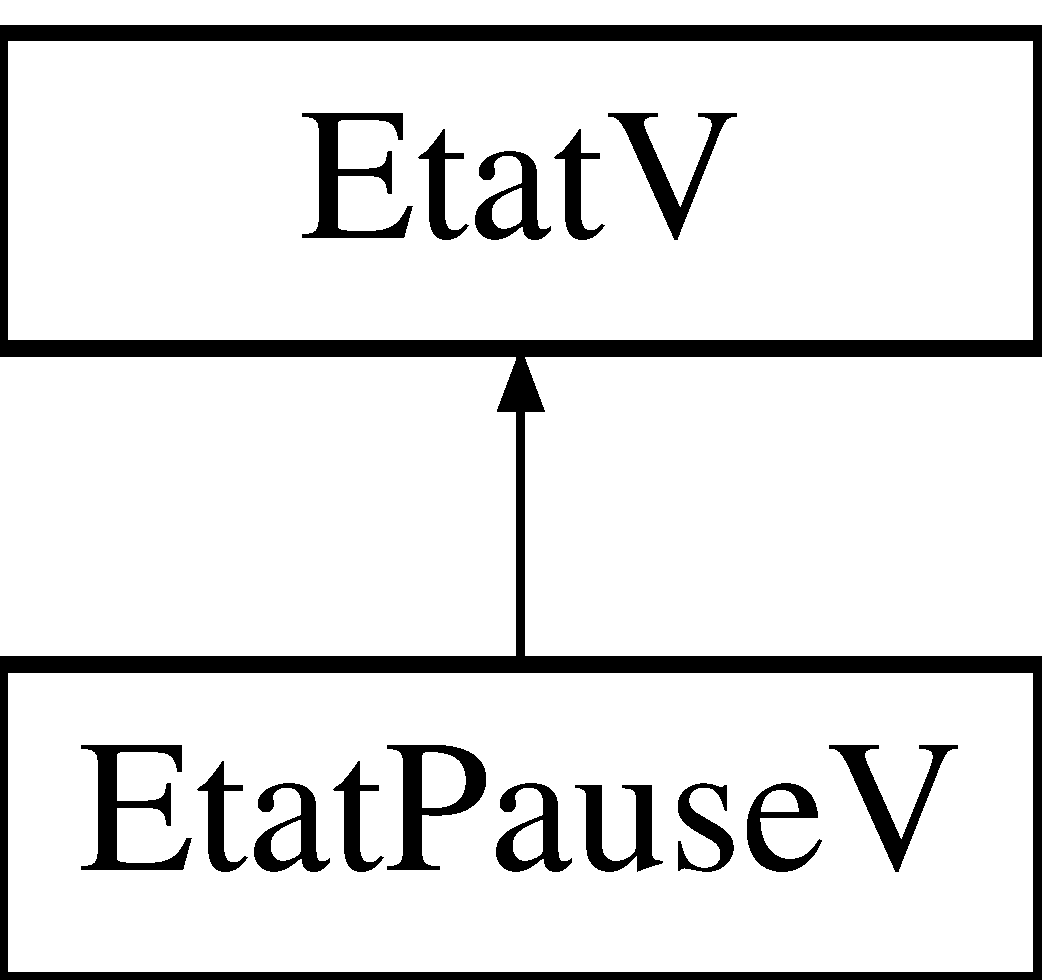
\includegraphics[height=2.000000cm]{classEtatPauseV}
\end{center}
\end{figure}
\subsection*{Fonctions membres publiques}
\begin{DoxyCompactItemize}
\item 
\hypertarget{classEtatPauseV_adc71aed982aab87ac55763db51b5a7d6}{\hyperlink{classEtatPauseV_adc71aed982aab87ac55763db51b5a7d6}{Etat\+Pause\+V} ()}\label{classEtatPauseV_adc71aed982aab87ac55763db51b5a7d6}

\begin{DoxyCompactList}\small\item\em Constructeur. \end{DoxyCompactList}\item 
\hyperlink{classEtatPauseV_aa8eab25d136fd125b0c7bb4307fd1b6e}{Etat\+Pause\+V} (\hyperlink{classVideo}{Video} $\ast$v)
\begin{DoxyCompactList}\small\item\em Constructeur. \end{DoxyCompactList}\item 
\hypertarget{classEtatPauseV_aa54762c0a9beb8a480328e496427f87e}{void \hyperlink{classEtatPauseV_aa54762c0a9beb8a480328e496427f87e}{utiliser\+Bouton\+Stop\+V} (sfe\+::\+Movie $\ast$movie)}\label{classEtatPauseV_aa54762c0a9beb8a480328e496427f87e}

\begin{DoxyCompactList}\small\item\em utiliser\+Bouton\+Stop\+V \+: passe la video dans l'état stop \end{DoxyCompactList}\item 
\hypertarget{classEtatPauseV_a31eab025c73198ba4659d007ee74e3ef}{void \hyperlink{classEtatPauseV_a31eab025c73198ba4659d007ee74e3ef}{utiliser\+Bouton\+Lecture\+V} (sfe\+::\+Movie $\ast$movie)}\label{classEtatPauseV_a31eab025c73198ba4659d007ee74e3ef}

\begin{DoxyCompactList}\small\item\em utiliser\+Bouton\+Lecture\+V \+: passe la video dans l'état lecture \end{DoxyCompactList}\item 
\hypertarget{classEtatPauseV_ac73e8e3bd58cdf51e143e5a8181fabc8}{void \hyperlink{classEtatPauseV_ac73e8e3bd58cdf51e143e5a8181fabc8}{afficher\+V} ()}\label{classEtatPauseV_ac73e8e3bd58cdf51e143e5a8181fabc8}

\begin{DoxyCompactList}\small\item\em afficher\+V \+: affiche l'état pause \end{DoxyCompactList}\end{DoxyCompactItemize}


\subsection{Description détaillée}


Définition à la ligne 13 du fichier etat\+Pause\+V.\+hpp.



\subsection{Documentation des constructeurs et destructeur}
\hypertarget{classEtatPauseV_aa8eab25d136fd125b0c7bb4307fd1b6e}{\index{Etat\+Pause\+V@{Etat\+Pause\+V}!Etat\+Pause\+V@{Etat\+Pause\+V}}
\index{Etat\+Pause\+V@{Etat\+Pause\+V}!Etat\+Pause\+V@{Etat\+Pause\+V}}
\subsubsection[{Etat\+Pause\+V}]{\setlength{\rightskip}{0pt plus 5cm}Etat\+Pause\+V\+::\+Etat\+Pause\+V (
\begin{DoxyParamCaption}
\item[{{\bf Video} $\ast$}]{v}
\end{DoxyParamCaption}
)}}\label{classEtatPauseV_aa8eab25d136fd125b0c7bb4307fd1b6e}


Constructeur. 


\begin{DoxyParams}{Paramètres}
{\em \hyperlink{classVideo}{Video}} & v \+: pointeur vers video \\
\hline
\end{DoxyParams}


La documentation de cette classe a été générée à partir du fichier suivant \+:\begin{DoxyCompactItemize}
\item 
src/\+State\+Video/\hyperlink{etatPauseV_8hpp}{etat\+Pause\+V.\+hpp}\end{DoxyCompactItemize}

\hypertarget{classEtatV}{\section{Référence de la classe Etat\+V}
\label{classEtatV}\index{Etat\+V@{Etat\+V}}
}
Graphe d'héritage de Etat\+V\+:\begin{figure}[H]
\begin{center}
\leavevmode
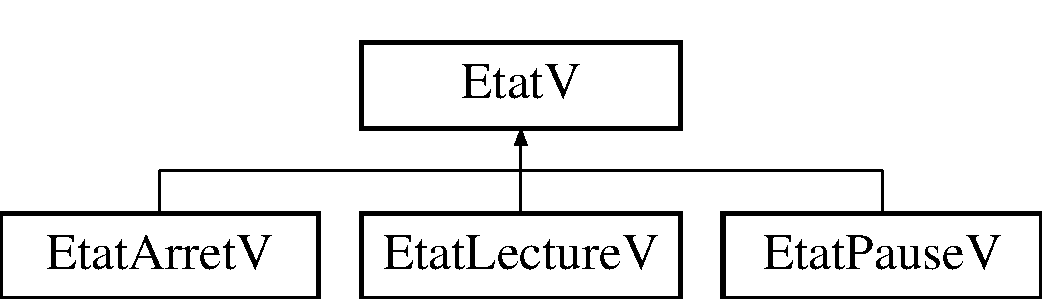
\includegraphics[height=2.000000cm]{classEtatV}
\end{center}
\end{figure}
\subsection*{Fonctions membres publiques}
\begin{DoxyCompactItemize}
\item 
\hypertarget{classEtatV_a28e8ff6a373f24518126adc084b80c65}{virtual void \hyperlink{classEtatV_a28e8ff6a373f24518126adc084b80c65}{utiliser\+Bouton\+Stop\+V} (sfe\+::\+Movie $\ast$movie)}\label{classEtatV_a28e8ff6a373f24518126adc084b80c65}

\begin{DoxyCompactList}\small\item\em utiliser\+Bouton\+Stop\+V \+: selon l'etat, effectue l'action du bouttonstop. Virtuel \end{DoxyCompactList}\item 
\hypertarget{classEtatV_a67aae8fba28db1225b49632e8c96ffcf}{virtual void \hyperlink{classEtatV_a67aae8fba28db1225b49632e8c96ffcf}{utiliser\+Bouton\+Pause\+V} (sfe\+::\+Movie $\ast$movie)}\label{classEtatV_a67aae8fba28db1225b49632e8c96ffcf}

\begin{DoxyCompactList}\small\item\em utiliser\+Bouton\+Pause\+V \+: selon l'etat, effectue l'action du bouttonpause. Virtuel \end{DoxyCompactList}\item 
\hypertarget{classEtatV_ad61eb5d733cf53024cdaa3c58d144752}{virtual void \hyperlink{classEtatV_ad61eb5d733cf53024cdaa3c58d144752}{utiliser\+Bouton\+Lecture\+V} (sfe\+::\+Movie $\ast$movie)}\label{classEtatV_ad61eb5d733cf53024cdaa3c58d144752}

\begin{DoxyCompactList}\small\item\em utiliser\+Bouton\+Lecture\+V \+: selon l'etat, effectue l'action du bouttonlecture. Virtuel \end{DoxyCompactList}\item 
\hypertarget{classEtatV_a25a68ea32060eb91e0a87624d594105c}{virtual void \hyperlink{classEtatV_a25a68ea32060eb91e0a87624d594105c}{afficher\+V} ()=0}\label{classEtatV_a25a68ea32060eb91e0a87624d594105c}

\begin{DoxyCompactList}\small\item\em afficher\+V \+: selon l'etat, affiche l'état de la vidéo. Virtuel \end{DoxyCompactList}\end{DoxyCompactItemize}


\subsection{Description détaillée}


Définition à la ligne 16 du fichier etat\+V.\+hpp.



La documentation de cette classe a été générée à partir du fichier suivant \+:\begin{DoxyCompactItemize}
\item 
src/\+State\+Video/\hyperlink{etatV_8hpp}{etat\+V.\+hpp}\end{DoxyCompactItemize}

\hypertarget{classFormat}{\section{Référence de la classe Format}
\label{classFormat}\index{Format@{Format}}
}
Graphe d'héritage de Format\+:\begin{figure}[H]
\begin{center}
\leavevmode
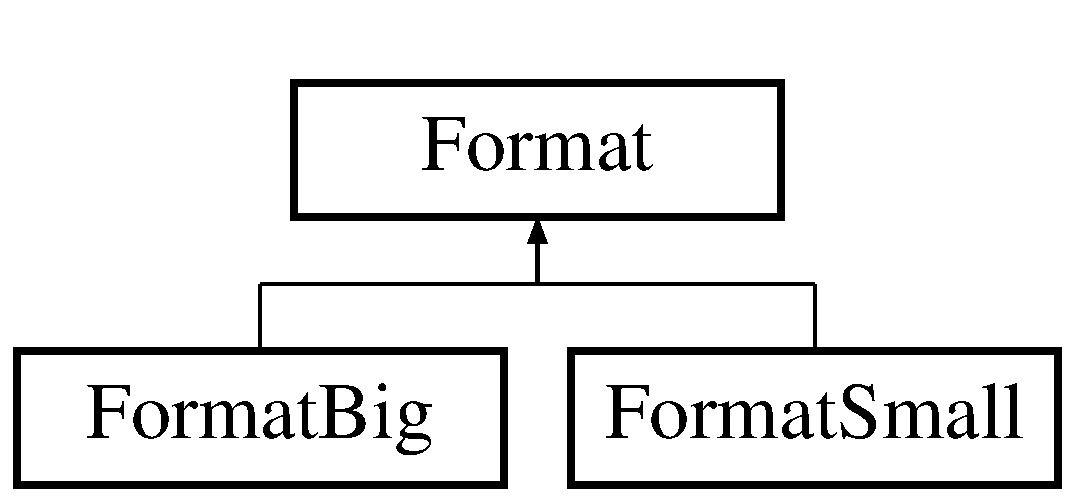
\includegraphics[height=2.000000cm]{classFormat}
\end{center}
\end{figure}
\subsection*{Fonctions membres publiques}
\begin{DoxyCompactItemize}
\item 
\hypertarget{classFormat_a07f4f6f3b4c5182a63d684c4a20b9d96}{virtual void {\bfseries create\+Format} ()=0}\label{classFormat_a07f4f6f3b4c5182a63d684c4a20b9d96}

\item 
virtual int \hyperlink{classFormat_ad5474275e85a8a47b5f0da28d7020283}{get\+Longueur} ()=0
\begin{DoxyCompactList}\small\item\em Getteur virtuel. \end{DoxyCompactList}\item 
virtual int \hyperlink{classFormat_a96150ade441ed68e056c20db86fd1607}{get\+Largeur} ()=0
\begin{DoxyCompactList}\small\item\em Getteur virtuel. \end{DoxyCompactList}\item 
virtual sf\+::\+Render\+Window $\ast$ \hyperlink{classFormat_a71418db76d6925708d403a1cd31b74f0}{get\+Window} ()=0
\begin{DoxyCompactList}\small\item\em Getteur virtuel. \end{DoxyCompactList}\end{DoxyCompactItemize}


\subsection{Description détaillée}


Définition à la ligne 14 du fichier format.\+hpp.



\subsection{Documentation des fonctions membres}
\hypertarget{classFormat_a96150ade441ed68e056c20db86fd1607}{\index{Format@{Format}!get\+Largeur@{get\+Largeur}}
\index{get\+Largeur@{get\+Largeur}!Format@{Format}}
\subsubsection[{get\+Largeur}]{\setlength{\rightskip}{0pt plus 5cm}virtual int Format\+::get\+Largeur (
\begin{DoxyParamCaption}
{}
\end{DoxyParamCaption}
)\hspace{0.3cm}{\ttfamily [pure virtual]}}}\label{classFormat_a96150ade441ed68e056c20db86fd1607}


Getteur virtuel. 

\begin{DoxyReturn}{Renvoie}
Retourne la largeur de la fenetre 
\end{DoxyReturn}


Implémenté dans \hyperlink{classFormatSmall_a64623731eba4359b6c2e32019aba42f7}{Format\+Small}, et \hyperlink{classFormatBig_acf985751797a389460bf4b5271ffbad4}{Format\+Big}.

\hypertarget{classFormat_ad5474275e85a8a47b5f0da28d7020283}{\index{Format@{Format}!get\+Longueur@{get\+Longueur}}
\index{get\+Longueur@{get\+Longueur}!Format@{Format}}
\subsubsection[{get\+Longueur}]{\setlength{\rightskip}{0pt plus 5cm}virtual int Format\+::get\+Longueur (
\begin{DoxyParamCaption}
{}
\end{DoxyParamCaption}
)\hspace{0.3cm}{\ttfamily [pure virtual]}}}\label{classFormat_ad5474275e85a8a47b5f0da28d7020283}


Getteur virtuel. 

\begin{DoxyReturn}{Renvoie}
Retourne la longueur de la fenetre 
\end{DoxyReturn}


Implémenté dans \hyperlink{classFormatSmall_a755b6b4f2c5f6c2fc8b5a49f08c0ec29}{Format\+Small}, et \hyperlink{classFormatBig_ae244731f051e849ce816189283d452f4}{Format\+Big}.

\hypertarget{classFormat_a71418db76d6925708d403a1cd31b74f0}{\index{Format@{Format}!get\+Window@{get\+Window}}
\index{get\+Window@{get\+Window}!Format@{Format}}
\subsubsection[{get\+Window}]{\setlength{\rightskip}{0pt plus 5cm}virtual sf\+::\+Render\+Window$\ast$ Format\+::get\+Window (
\begin{DoxyParamCaption}
{}
\end{DoxyParamCaption}
)\hspace{0.3cm}{\ttfamily [pure virtual]}}}\label{classFormat_a71418db76d6925708d403a1cd31b74f0}


Getteur virtuel. 

\begin{DoxyReturn}{Renvoie}
Retourne la fenetre de type Render\+Window 
\end{DoxyReturn}


Implémenté dans \hyperlink{classFormatSmall_ab15677846852366fb6dbea77dc22e82c}{Format\+Small}, et \hyperlink{classFormatBig_a48f6f2efc1d7d40f7562b8f1430f36c7}{Format\+Big}.



La documentation de cette classe a été générée à partir du fichier suivant \+:\begin{DoxyCompactItemize}
\item 
src/\+Abstract\+Factory/\hyperlink{format_8hpp}{format.\+hpp}\end{DoxyCompactItemize}

\hypertarget{classFormatBig}{\section{Référence de la classe Format\+Big}
\label{classFormatBig}\index{Format\+Big@{Format\+Big}}
}
Graphe d'héritage de Format\+Big\+:\begin{figure}[H]
\begin{center}
\leavevmode
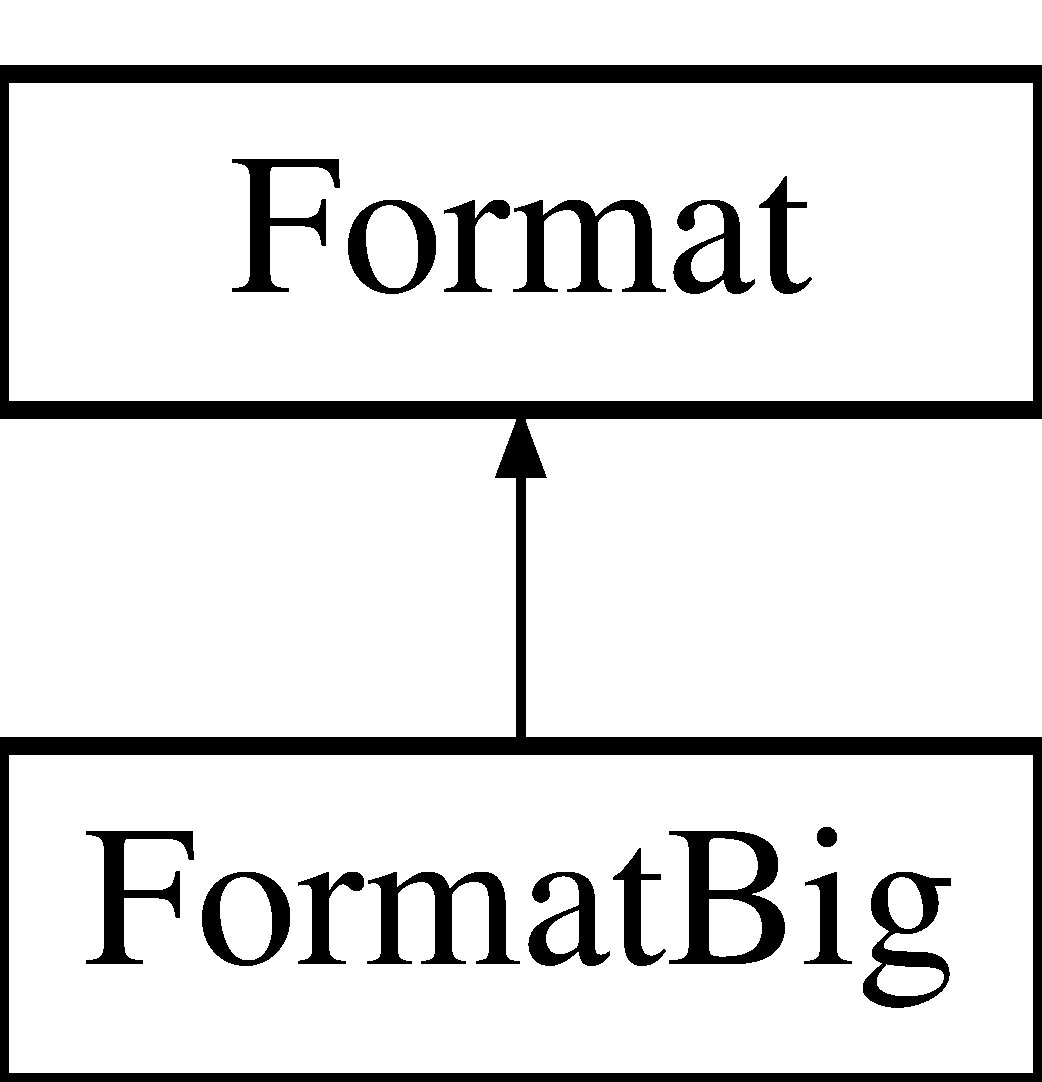
\includegraphics[height=2.000000cm]{classFormatBig}
\end{center}
\end{figure}
\subsection*{Fonctions membres publiques}
\begin{DoxyCompactItemize}
\item 
\hypertarget{classFormatBig_a705324cfcf29ccce442adbd5b327b821}{\hyperlink{classFormatBig_a705324cfcf29ccce442adbd5b327b821}{Format\+Big} ()}\label{classFormatBig_a705324cfcf29ccce442adbd5b327b821}

\begin{DoxyCompactList}\small\item\em Constructeur. \end{DoxyCompactList}\item 
void \hyperlink{classFormatBig_a1c0bbd51c2093997c75624682dba8772}{create\+Format} ()
\begin{DoxyCompactList}\small\item\em Crée le format grand. \end{DoxyCompactList}\item 
int \hyperlink{classFormatBig_ae244731f051e849ce816189283d452f4}{get\+Longueur} ()
\begin{DoxyCompactList}\small\item\em Getteur. \end{DoxyCompactList}\item 
int \hyperlink{classFormatBig_acf985751797a389460bf4b5271ffbad4}{get\+Largeur} ()
\begin{DoxyCompactList}\small\item\em Getteur. \end{DoxyCompactList}\item 
sf\+::\+Render\+Window $\ast$ \hyperlink{classFormatBig_a48f6f2efc1d7d40f7562b8f1430f36c7}{get\+Window} ()
\begin{DoxyCompactList}\small\item\em Getteur. \end{DoxyCompactList}\end{DoxyCompactItemize}


\subsection{Description détaillée}


Définition à la ligne 13 du fichier format\+Big.\+hpp.



\subsection{Documentation des fonctions membres}
\hypertarget{classFormatBig_a1c0bbd51c2093997c75624682dba8772}{\index{Format\+Big@{Format\+Big}!create\+Format@{create\+Format}}
\index{create\+Format@{create\+Format}!Format\+Big@{Format\+Big}}
\subsubsection[{create\+Format}]{\setlength{\rightskip}{0pt plus 5cm}void Format\+Big\+::create\+Format (
\begin{DoxyParamCaption}
{}
\end{DoxyParamCaption}
)\hspace{0.3cm}{\ttfamily [virtual]}}}\label{classFormatBig_a1c0bbd51c2093997c75624682dba8772}


Crée le format grand. 

\begin{DoxyReturn}{Renvoie}
Un \hyperlink{classFormat}{Format} 
\end{DoxyReturn}


Implémente \hyperlink{classFormat_a07f4f6f3b4c5182a63d684c4a20b9d96}{Format}.

\hypertarget{classFormatBig_acf985751797a389460bf4b5271ffbad4}{\index{Format\+Big@{Format\+Big}!get\+Largeur@{get\+Largeur}}
\index{get\+Largeur@{get\+Largeur}!Format\+Big@{Format\+Big}}
\subsubsection[{get\+Largeur}]{\setlength{\rightskip}{0pt plus 5cm}int Format\+Big\+::get\+Largeur (
\begin{DoxyParamCaption}
{}
\end{DoxyParamCaption}
)\hspace{0.3cm}{\ttfamily [virtual]}}}\label{classFormatBig_acf985751797a389460bf4b5271ffbad4}


Getteur. 

\begin{DoxyReturn}{Renvoie}
Retourne la largeur de la fenetre 
\end{DoxyReturn}


Implémente \hyperlink{classFormat_a96150ade441ed68e056c20db86fd1607}{Format}.

\hypertarget{classFormatBig_ae244731f051e849ce816189283d452f4}{\index{Format\+Big@{Format\+Big}!get\+Longueur@{get\+Longueur}}
\index{get\+Longueur@{get\+Longueur}!Format\+Big@{Format\+Big}}
\subsubsection[{get\+Longueur}]{\setlength{\rightskip}{0pt plus 5cm}int Format\+Big\+::get\+Longueur (
\begin{DoxyParamCaption}
{}
\end{DoxyParamCaption}
)\hspace{0.3cm}{\ttfamily [virtual]}}}\label{classFormatBig_ae244731f051e849ce816189283d452f4}


Getteur. 

\begin{DoxyReturn}{Renvoie}
Retourne la longueur de la fenetre 
\end{DoxyReturn}


Implémente \hyperlink{classFormat_ad5474275e85a8a47b5f0da28d7020283}{Format}.

\hypertarget{classFormatBig_a48f6f2efc1d7d40f7562b8f1430f36c7}{\index{Format\+Big@{Format\+Big}!get\+Window@{get\+Window}}
\index{get\+Window@{get\+Window}!Format\+Big@{Format\+Big}}
\subsubsection[{get\+Window}]{\setlength{\rightskip}{0pt plus 5cm}sf\+::\+Render\+Window$\ast$ Format\+Big\+::get\+Window (
\begin{DoxyParamCaption}
{}
\end{DoxyParamCaption}
)\hspace{0.3cm}{\ttfamily [virtual]}}}\label{classFormatBig_a48f6f2efc1d7d40f7562b8f1430f36c7}


Getteur. 

\begin{DoxyReturn}{Renvoie}
Retourne la fenetre de type Render\+Window 
\end{DoxyReturn}


Implémente \hyperlink{classFormat_a71418db76d6925708d403a1cd31b74f0}{Format}.



La documentation de cette classe a été générée à partir du fichier suivant \+:\begin{DoxyCompactItemize}
\item 
src/\+Abstract\+Factory/\hyperlink{formatBig_8hpp}{format\+Big.\+hpp}\end{DoxyCompactItemize}

\hypertarget{classFormatSmall}{\section{Référence de la classe Format\+Small}
\label{classFormatSmall}\index{Format\+Small@{Format\+Small}}
}
Graphe d'héritage de Format\+Small\+:\begin{figure}[H]
\begin{center}
\leavevmode
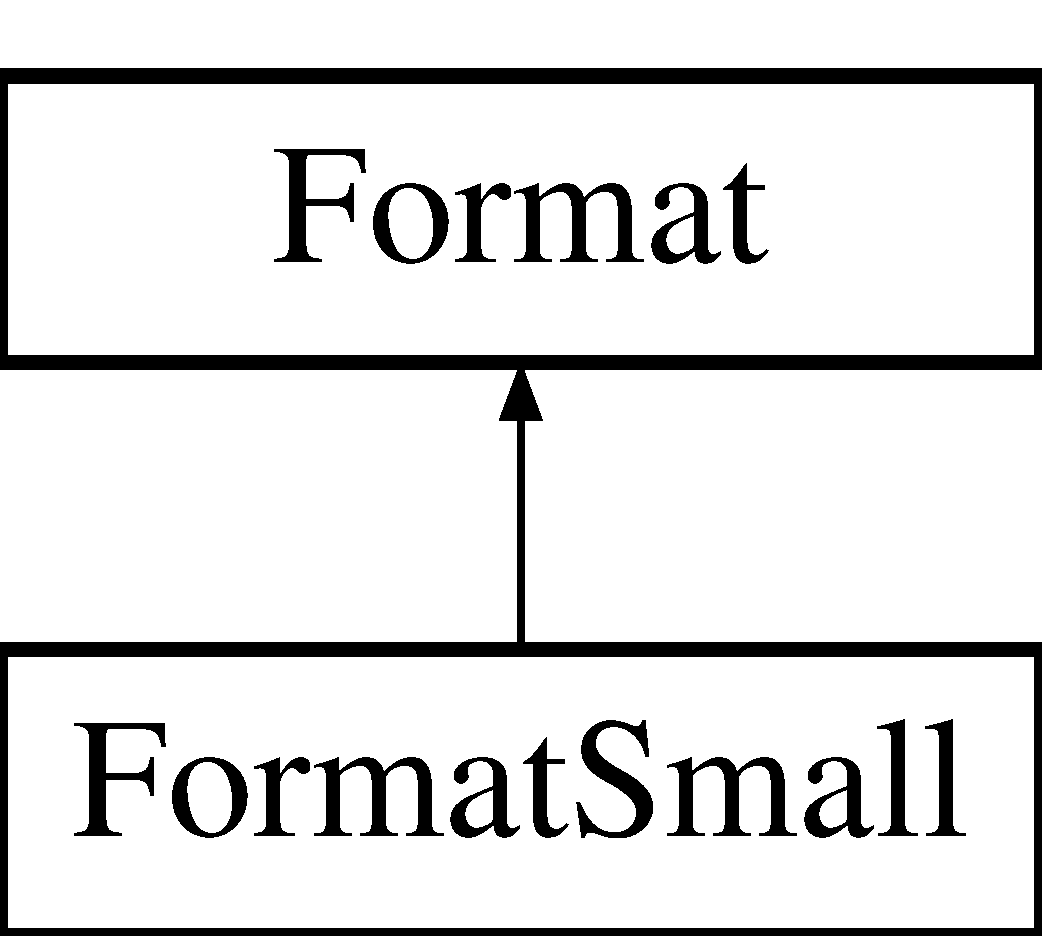
\includegraphics[height=2.000000cm]{classFormatSmall}
\end{center}
\end{figure}
\subsection*{Fonctions membres publiques}
\begin{DoxyCompactItemize}
\item 
\hypertarget{classFormatSmall_aca8b600f88876ec205174cc61e65cca2}{\hyperlink{classFormatSmall_aca8b600f88876ec205174cc61e65cca2}{Format\+Small} ()}\label{classFormatSmall_aca8b600f88876ec205174cc61e65cca2}

\begin{DoxyCompactList}\small\item\em Constructeur. \end{DoxyCompactList}\item 
void \hyperlink{classFormatSmall_a985c6ed4ea1e16c267e0af5523dbba1f}{create\+Format} ()
\begin{DoxyCompactList}\small\item\em Crée le format petit. \end{DoxyCompactList}\item 
int \hyperlink{classFormatSmall_a755b6b4f2c5f6c2fc8b5a49f08c0ec29}{get\+Longueur} ()
\begin{DoxyCompactList}\small\item\em Accesseur longueur. \end{DoxyCompactList}\item 
int \hyperlink{classFormatSmall_a64623731eba4359b6c2e32019aba42f7}{get\+Largeur} ()
\begin{DoxyCompactList}\small\item\em Accesseur largeur. \end{DoxyCompactList}\item 
sf\+::\+Render\+Window $\ast$ \hyperlink{classFormatSmall_ab15677846852366fb6dbea77dc22e82c}{get\+Window} ()
\begin{DoxyCompactList}\small\item\em Accesseyr fenetre. \end{DoxyCompactList}\end{DoxyCompactItemize}


\subsection{Description détaillée}


Définition à la ligne 13 du fichier format\+Small.\+hpp.



\subsection{Documentation des fonctions membres}
\hypertarget{classFormatSmall_a985c6ed4ea1e16c267e0af5523dbba1f}{\index{Format\+Small@{Format\+Small}!create\+Format@{create\+Format}}
\index{create\+Format@{create\+Format}!Format\+Small@{Format\+Small}}
\subsubsection[{create\+Format}]{\setlength{\rightskip}{0pt plus 5cm}void Format\+Small\+::create\+Format (
\begin{DoxyParamCaption}
{}
\end{DoxyParamCaption}
)\hspace{0.3cm}{\ttfamily [virtual]}}}\label{classFormatSmall_a985c6ed4ea1e16c267e0af5523dbba1f}


Crée le format petit. 

\begin{DoxyReturn}{Renvoie}
Un \hyperlink{classFormat}{Format} 
\end{DoxyReturn}


Implémente \hyperlink{classFormat_a07f4f6f3b4c5182a63d684c4a20b9d96}{Format}.

\hypertarget{classFormatSmall_a64623731eba4359b6c2e32019aba42f7}{\index{Format\+Small@{Format\+Small}!get\+Largeur@{get\+Largeur}}
\index{get\+Largeur@{get\+Largeur}!Format\+Small@{Format\+Small}}
\subsubsection[{get\+Largeur}]{\setlength{\rightskip}{0pt plus 5cm}int Format\+Small\+::get\+Largeur (
\begin{DoxyParamCaption}
{}
\end{DoxyParamCaption}
)\hspace{0.3cm}{\ttfamily [virtual]}}}\label{classFormatSmall_a64623731eba4359b6c2e32019aba42f7}


Accesseur largeur. 

\begin{DoxyReturn}{Renvoie}
Retourne la largeur de la fenetre 
\end{DoxyReturn}


Implémente \hyperlink{classFormat_a96150ade441ed68e056c20db86fd1607}{Format}.

\hypertarget{classFormatSmall_a755b6b4f2c5f6c2fc8b5a49f08c0ec29}{\index{Format\+Small@{Format\+Small}!get\+Longueur@{get\+Longueur}}
\index{get\+Longueur@{get\+Longueur}!Format\+Small@{Format\+Small}}
\subsubsection[{get\+Longueur}]{\setlength{\rightskip}{0pt plus 5cm}int Format\+Small\+::get\+Longueur (
\begin{DoxyParamCaption}
{}
\end{DoxyParamCaption}
)\hspace{0.3cm}{\ttfamily [virtual]}}}\label{classFormatSmall_a755b6b4f2c5f6c2fc8b5a49f08c0ec29}


Accesseur longueur. 

\begin{DoxyReturn}{Renvoie}
Retourne la longueur de la fenetre 
\end{DoxyReturn}


Implémente \hyperlink{classFormat_ad5474275e85a8a47b5f0da28d7020283}{Format}.

\hypertarget{classFormatSmall_ab15677846852366fb6dbea77dc22e82c}{\index{Format\+Small@{Format\+Small}!get\+Window@{get\+Window}}
\index{get\+Window@{get\+Window}!Format\+Small@{Format\+Small}}
\subsubsection[{get\+Window}]{\setlength{\rightskip}{0pt plus 5cm}sf\+::\+Render\+Window$\ast$ Format\+Small\+::get\+Window (
\begin{DoxyParamCaption}
{}
\end{DoxyParamCaption}
)\hspace{0.3cm}{\ttfamily [virtual]}}}\label{classFormatSmall_ab15677846852366fb6dbea77dc22e82c}


Accesseyr fenetre. 

\begin{DoxyReturn}{Renvoie}
Retourne la fenetre de type Render\+Window 
\end{DoxyReturn}


Implémente \hyperlink{classFormat_a71418db76d6925708d403a1cd31b74f0}{Format}.



La documentation de cette classe a été générée à partir du fichier suivant \+:\begin{DoxyCompactItemize}
\item 
src/\+Abstract\+Factory/\hyperlink{formatSmall_8hpp}{format\+Small.\+hpp}\end{DoxyCompactItemize}

\hypertarget{classImage}{\section{Référence de la classe Image}
\label{classImage}\index{Image@{Image}}
}
\subsection*{Fonctions membres publiques}
\begin{DoxyCompactItemize}
\item 
\hypertarget{classImage_a2e8f8d5193e5c6e49de276f9d1f4bdde}{{\bfseries Image} (\hyperlink{classImageInterfaceFactory}{Image\+Interface\+Factory} $\ast$ii\+Fact)}\label{classImage_a2e8f8d5193e5c6e49de276f9d1f4bdde}

\item 
\hypertarget{classImage_a4d957034ad17e3911a4d9f7decdda22c}{void {\bfseries afficher} ()}\label{classImage_a4d957034ad17e3911a4d9f7decdda22c}

\item 
\hypertarget{classImage_a0ee0602472090d8723d081849dfe6e27}{void {\bfseries run} ()}\label{classImage_a0ee0602472090d8723d081849dfe6e27}

\end{DoxyCompactItemize}


\subsection{Description détaillée}


Définition à la ligne 4 du fichier image.\+hpp.



La documentation de cette classe a été générée à partir du fichier suivant \+:\begin{DoxyCompactItemize}
\item 
src/image.\+hpp\end{DoxyCompactItemize}

\hypertarget{classImageInterfaceFactory}{\section{Référence de la classe Image\+Interface\+Factory}
\label{classImageInterfaceFactory}\index{Image\+Interface\+Factory@{Image\+Interface\+Factory}}
}
Graphe d'héritage de Image\+Interface\+Factory\+:\begin{figure}[H]
\begin{center}
\leavevmode
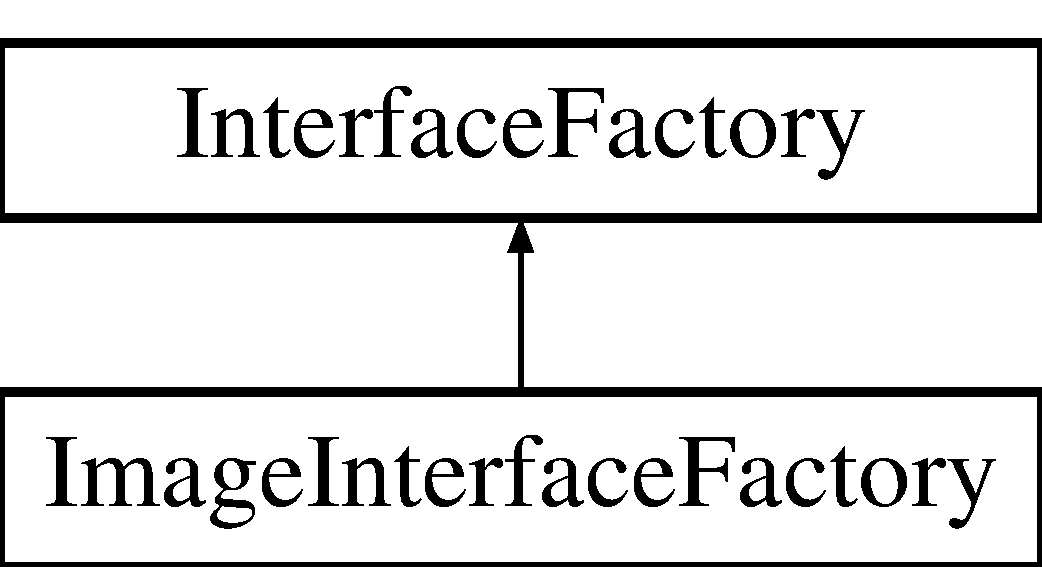
\includegraphics[height=2.000000cm]{classImageInterfaceFactory}
\end{center}
\end{figure}
\subsection*{Fonctions membres publiques}
\begin{DoxyCompactItemize}
\item 
\hyperlink{classInterface}{Interface} \hyperlink{classImageInterfaceFactory_ace6a51fa023edcf9c99aee2a7e74ca5a}{create\+Interface} (\hyperlink{classButtons}{Buttons} $\ast$b, \hyperlink{classFormat}{Format} $\ast$f)
\begin{DoxyCompactList}\small\item\em Crée l'interface adéquate à la lecture d'un fichier image. \end{DoxyCompactList}\end{DoxyCompactItemize}


\subsection{Description détaillée}


Définition à la ligne 16 du fichier image\+Interface\+Factory.\+hpp.



\subsection{Documentation des fonctions membres}
\hypertarget{classImageInterfaceFactory_ace6a51fa023edcf9c99aee2a7e74ca5a}{\index{Image\+Interface\+Factory@{Image\+Interface\+Factory}!create\+Interface@{create\+Interface}}
\index{create\+Interface@{create\+Interface}!Image\+Interface\+Factory@{Image\+Interface\+Factory}}
\subsubsection[{create\+Interface}]{\setlength{\rightskip}{0pt plus 5cm}{\bf Interface} Image\+Interface\+Factory\+::create\+Interface (
\begin{DoxyParamCaption}
\item[{{\bf Buttons} $\ast$}]{b, }
\item[{{\bf Format} $\ast$}]{f}
\end{DoxyParamCaption}
)\hspace{0.3cm}{\ttfamily [virtual]}}}\label{classImageInterfaceFactory_ace6a51fa023edcf9c99aee2a7e74ca5a}


Crée l'interface adéquate à la lecture d'un fichier image. 


\begin{DoxyParams}{Paramètres}
{\em \hyperlink{classButtonsI}{Buttons\+I}} & bi, \hyperlink{classFormatBig}{Format\+Big} fb \\
\hline
\end{DoxyParams}


Implémente \hyperlink{classInterfaceFactory}{Interface\+Factory}.



La documentation de cette classe a été générée à partir du fichier suivant \+:\begin{DoxyCompactItemize}
\item 
src/\+Abstract\+Factory/\hyperlink{imageInterfaceFactory_8hpp}{image\+Interface\+Factory.\+hpp}\end{DoxyCompactItemize}

\hypertarget{classInterface}{\section{Référence de la classe Interface}
\label{classInterface}\index{Interface@{Interface}}
}
\subsection*{Fonctions membres publiques}
\begin{DoxyCompactItemize}
\item 
\hypertarget{classInterface_a4406d74c75bdfe150bf72be1f1cda8b1}{\hyperlink{classInterface_a4406d74c75bdfe150bf72be1f1cda8b1}{Interface} ()}\label{classInterface_a4406d74c75bdfe150bf72be1f1cda8b1}

\begin{DoxyCompactList}\small\item\em Constructeur. \end{DoxyCompactList}\item 
\hypertarget{classInterface_a131417f8ff9a3d96a3c301a324697043}{\hyperlink{classInterface_a131417f8ff9a3d96a3c301a324697043}{Interface} (\hyperlink{classButtons}{Buttons} $\ast$b, \hyperlink{classFormat}{Format} $\ast$f, tgui\+::\+Gui $\ast$gui)}\label{classInterface_a131417f8ff9a3d96a3c301a324697043}

\begin{DoxyCompactList}\small\item\em Constructeur. \end{DoxyCompactList}\item 
\hyperlink{classButtons}{Buttons} $\ast$ \hyperlink{classInterface_a90f1a995485ef1b9084701a7c7e44fd5}{get\+Buttons} ()
\begin{DoxyCompactList}\small\item\em Getteur. \end{DoxyCompactList}\item 
\hyperlink{classFormat}{Format} $\ast$ \hyperlink{classInterface_a09d8ee2dadc6a2e37437f1ead14f2816}{get\+Format} ()
\begin{DoxyCompactList}\small\item\em Getteur. \end{DoxyCompactList}\item 
tgui\+::\+Gui $\ast$ \hyperlink{classInterface_af732676b1b5e04a4401a7c5eaa7f8ce6}{get\+Gui} ()
\begin{DoxyCompactList}\small\item\em Getteur. \end{DoxyCompactList}\end{DoxyCompactItemize}


\subsection{Description détaillée}


Définition à la ligne 17 du fichier interface.\+hpp.



\subsection{Documentation des fonctions membres}
\hypertarget{classInterface_a90f1a995485ef1b9084701a7c7e44fd5}{\index{Interface@{Interface}!get\+Buttons@{get\+Buttons}}
\index{get\+Buttons@{get\+Buttons}!Interface@{Interface}}
\subsubsection[{get\+Buttons}]{\setlength{\rightskip}{0pt plus 5cm}{\bf Buttons}$\ast$ Interface\+::get\+Buttons (
\begin{DoxyParamCaption}
{}
\end{DoxyParamCaption}
)}}\label{classInterface_a90f1a995485ef1b9084701a7c7e44fd5}


Getteur. 

\begin{DoxyReturn}{Renvoie}
Retourne les boutons créés 
\end{DoxyReturn}
\hypertarget{classInterface_a09d8ee2dadc6a2e37437f1ead14f2816}{\index{Interface@{Interface}!get\+Format@{get\+Format}}
\index{get\+Format@{get\+Format}!Interface@{Interface}}
\subsubsection[{get\+Format}]{\setlength{\rightskip}{0pt plus 5cm}{\bf Format}$\ast$ Interface\+::get\+Format (
\begin{DoxyParamCaption}
{}
\end{DoxyParamCaption}
)}}\label{classInterface_a09d8ee2dadc6a2e37437f1ead14f2816}


Getteur. 

\begin{DoxyReturn}{Renvoie}
Retourne le format créé 
\end{DoxyReturn}
\hypertarget{classInterface_af732676b1b5e04a4401a7c5eaa7f8ce6}{\index{Interface@{Interface}!get\+Gui@{get\+Gui}}
\index{get\+Gui@{get\+Gui}!Interface@{Interface}}
\subsubsection[{get\+Gui}]{\setlength{\rightskip}{0pt plus 5cm}tgui\+::\+Gui$\ast$ Interface\+::get\+Gui (
\begin{DoxyParamCaption}
{}
\end{DoxyParamCaption}
)}}\label{classInterface_af732676b1b5e04a4401a7c5eaa7f8ce6}


Getteur. 

\begin{DoxyReturn}{Renvoie}
Retourne le gui de l'interface 
\end{DoxyReturn}


La documentation de cette classe a été générée à partir du fichier suivant \+:\begin{DoxyCompactItemize}
\item 
src/\+Abstract\+Factory/\hyperlink{interface_8hpp}{interface.\+hpp}\end{DoxyCompactItemize}

\hypertarget{classInterfaceFactory}{\section{Référence de la classe Interface\+Factory}
\label{classInterfaceFactory}\index{Interface\+Factory@{Interface\+Factory}}
}
Graphe d'héritage de Interface\+Factory\+:\begin{figure}[H]
\begin{center}
\leavevmode
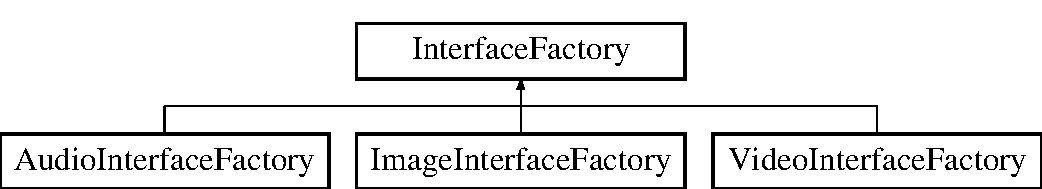
\includegraphics[height=2.000000cm]{classInterfaceFactory}
\end{center}
\end{figure}
\subsection*{Fonctions membres publiques}
\begin{DoxyCompactItemize}
\item 
\hypertarget{classInterfaceFactory_a043c593647071e277c897a5416221de0}{virtual \hyperlink{classInterface}{Interface} {\bfseries create\+Interface} (\hyperlink{classButtons}{Buttons} $\ast$b, \hyperlink{classFormat}{Format} $\ast$f)=0}\label{classInterfaceFactory_a043c593647071e277c897a5416221de0}

\end{DoxyCompactItemize}


\subsection{Description détaillée}


Définition à la ligne 13 du fichier interface\+Factory.\+hpp.



La documentation de cette classe a été générée à partir du fichier suivant \+:\begin{DoxyCompactItemize}
\item 
src/\+Abstract\+Factory/\hyperlink{interfaceFactory_8hpp}{interface\+Factory.\+hpp}\end{DoxyCompactItemize}

\hypertarget{classObserver}{\section{Référence de la classe Observer}
\label{classObserver}\index{Observer@{Observer}}
}
Graphe d'héritage de Observer\+:\begin{figure}[H]
\begin{center}
\leavevmode
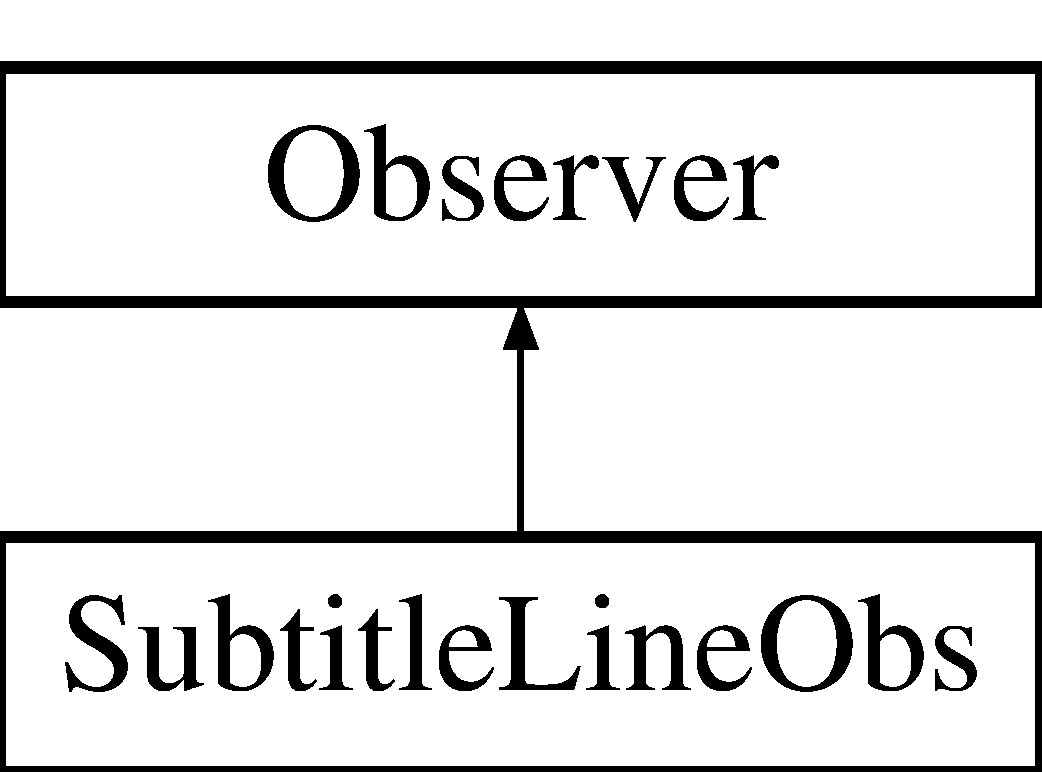
\includegraphics[height=2.000000cm]{classObserver}
\end{center}
\end{figure}
\subsection*{Fonctions membres publiques}
\begin{DoxyCompactItemize}
\item 
\hypertarget{classObserver_a62bb58b07e0b61972acdf7c1d51de98d}{virtual void {\bfseries update} (std\+::string d)=0}\label{classObserver_a62bb58b07e0b61972acdf7c1d51de98d}

\end{DoxyCompactItemize}


\subsection{Description détaillée}


Définition à la ligne 15 du fichier Observer.\+hpp.



La documentation de cette classe a été générée à partir du fichier suivant \+:\begin{DoxyCompactItemize}
\item 
src/\+Observer/\hyperlink{Observer_8hpp}{Observer.\+hpp}\end{DoxyCompactItemize}

\hypertarget{classSubject}{\section{Référence de la classe Subject}
\label{classSubject}\index{Subject@{Subject}}
}
Graphe d'héritage de Subject\+:\begin{figure}[H]
\begin{center}
\leavevmode
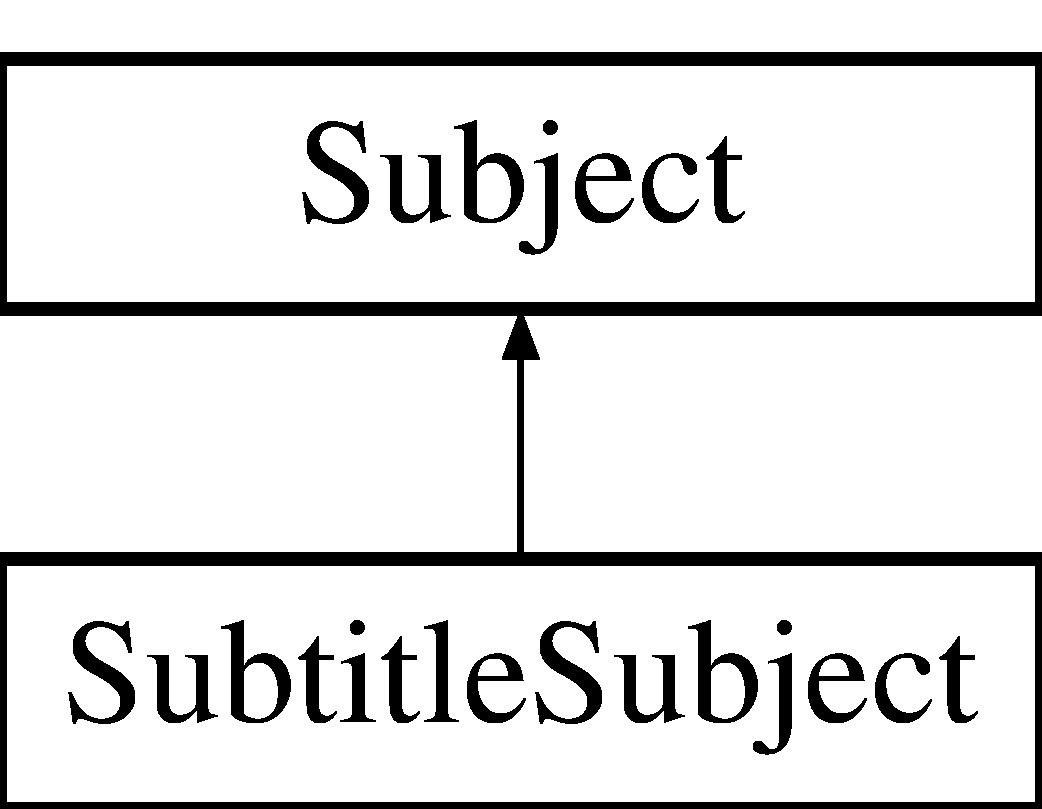
\includegraphics[height=2.000000cm]{classSubject}
\end{center}
\end{figure}
\subsection*{Fonctions membres publiques}
\begin{DoxyCompactItemize}
\item 
virtual int \hyperlink{classSubject_aecac0cb2c69c2d18db0e9433f580bde7}{add\+Obs} (\hyperlink{classObserver}{Observer} $\ast$o)=0
\begin{DoxyCompactList}\small\item\em Ajout un \hyperlink{classObserver}{Observer}. Virtuel. \end{DoxyCompactList}\item 
virtual int \hyperlink{classSubject_a4455d35d683c0005035121c7442b3a55}{remove\+Obs} (\hyperlink{classObserver}{Observer} $\ast$o)=0
\begin{DoxyCompactList}\small\item\em Supprime un \hyperlink{classObserver}{Observer}. Virtuel. \end{DoxyCompactList}\item 
\hypertarget{classSubject_a421d620f3f93365bfd57cd1e9165e501}{virtual void \hyperlink{classSubject_a421d620f3f93365bfd57cd1e9165e501}{notify\+Obs} ()=0}\label{classSubject_a421d620f3f93365bfd57cd1e9165e501}

\begin{DoxyCompactList}\small\item\em Notifie l'ensemble des observers ajoutés à au vecteur. Virtuel. \end{DoxyCompactList}\end{DoxyCompactItemize}


\subsection{Description détaillée}


Définition à la ligne 14 du fichier Subject.\+hpp.



\subsection{Documentation des fonctions membres}
\hypertarget{classSubject_aecac0cb2c69c2d18db0e9433f580bde7}{\index{Subject@{Subject}!add\+Obs@{add\+Obs}}
\index{add\+Obs@{add\+Obs}!Subject@{Subject}}
\subsubsection[{add\+Obs}]{\setlength{\rightskip}{0pt plus 5cm}virtual int Subject\+::add\+Obs (
\begin{DoxyParamCaption}
\item[{{\bf Observer} $\ast$}]{o}
\end{DoxyParamCaption}
)\hspace{0.3cm}{\ttfamily [pure virtual]}}}\label{classSubject_aecac0cb2c69c2d18db0e9433f580bde7}


Ajout un \hyperlink{classObserver}{Observer}. Virtuel. 


\begin{DoxyParams}{Paramètres}
{\em l'observer} & à ajouter \\
\hline
\end{DoxyParams}
\begin{DoxyReturn}{Renvoie}
\+\_\+retour 1 si l'observer a été ajouté 
\end{DoxyReturn}


Implémenté dans \hyperlink{classSubtitleSubject_afc89e947aab454357dce8ea2f80403ee}{Subtitle\+Subject}.

\hypertarget{classSubject_a4455d35d683c0005035121c7442b3a55}{\index{Subject@{Subject}!remove\+Obs@{remove\+Obs}}
\index{remove\+Obs@{remove\+Obs}!Subject@{Subject}}
\subsubsection[{remove\+Obs}]{\setlength{\rightskip}{0pt plus 5cm}virtual int Subject\+::remove\+Obs (
\begin{DoxyParamCaption}
\item[{{\bf Observer} $\ast$}]{o}
\end{DoxyParamCaption}
)\hspace{0.3cm}{\ttfamily [pure virtual]}}}\label{classSubject_a4455d35d683c0005035121c7442b3a55}


Supprime un \hyperlink{classObserver}{Observer}. Virtuel. 


\begin{DoxyParams}{Paramètres}
{\em l'observer} & à supprimer \\
\hline
\end{DoxyParams}
\begin{DoxyReturn}{Renvoie}
\+\_\+retour 1 si l'observer a été trouvé et supprimé sinon -\/1 
\end{DoxyReturn}


Implémenté dans \hyperlink{classSubtitleSubject_a60e75a2a34275176aaea81738ee4879d}{Subtitle\+Subject}.



La documentation de cette classe a été générée à partir du fichier suivant \+:\begin{DoxyCompactItemize}
\item 
src/\+Observer/Subject.\+hpp\end{DoxyCompactItemize}

\hypertarget{classSubtitleLineObs}{\section{Référence de la classe Subtitle\+Line\+Obs}
\label{classSubtitleLineObs}\index{Subtitle\+Line\+Obs@{Subtitle\+Line\+Obs}}
}
Graphe d'héritage de Subtitle\+Line\+Obs\+:\begin{figure}[H]
\begin{center}
\leavevmode
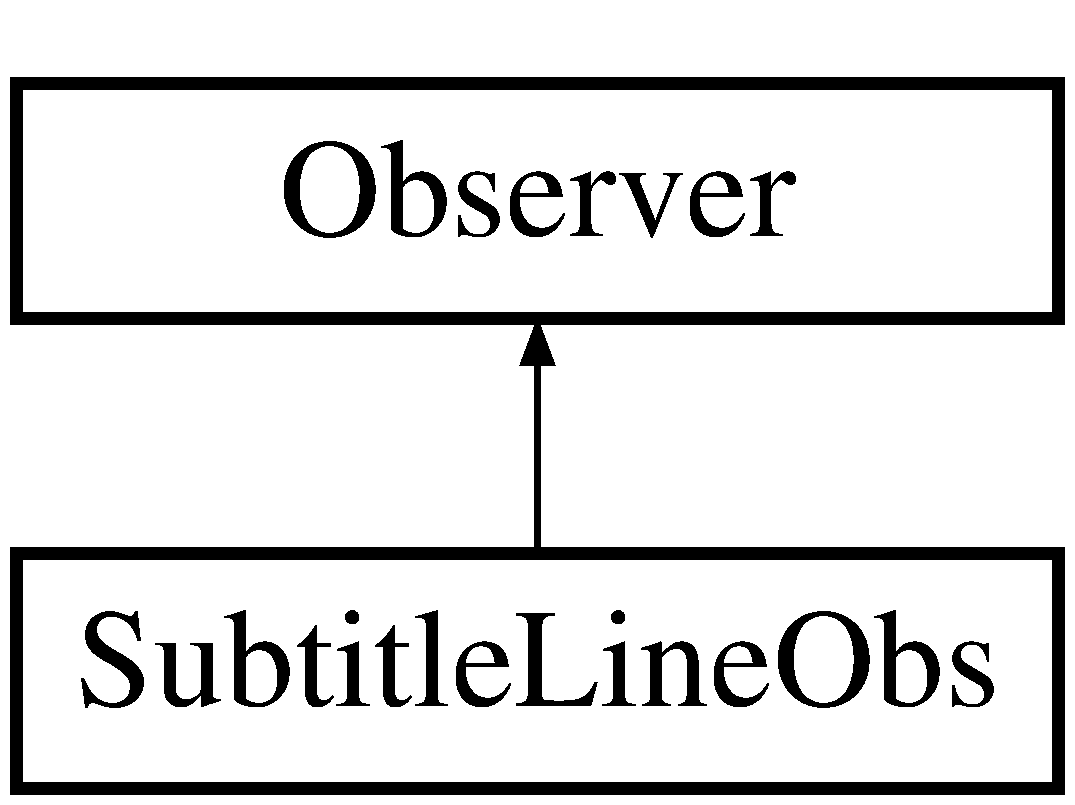
\includegraphics[height=2.000000cm]{classSubtitleLineObs}
\end{center}
\end{figure}
\subsection*{Fonctions membres publiques}
\begin{DoxyCompactItemize}
\item 
\hypertarget{classSubtitleLineObs_a3bfe134db1948a08b869f6671070ed1d}{{\bfseries Subtitle\+Line\+Obs} (\hyperlink{classSubject}{Subject} $\ast$s, tgui\+::\+Gui $\ast$gui)}\label{classSubtitleLineObs_a3bfe134db1948a08b869f6671070ed1d}

\item 
\hypertarget{classSubtitleLineObs_a74983bcd67169fa7cabd03f156affa04}{std\+::string {\bfseries get\+Data} ()}\label{classSubtitleLineObs_a74983bcd67169fa7cabd03f156affa04}

\item 
\hypertarget{classSubtitleLineObs_a57cab0db5ead28c8692f3793f5f50270}{void {\bfseries display} ()}\label{classSubtitleLineObs_a57cab0db5ead28c8692f3793f5f50270}

\item 
\hypertarget{classSubtitleLineObs_a5aab5a727bb01f5d8adc5d31a7521b13}{void {\bfseries update} (std\+::string d)}\label{classSubtitleLineObs_a5aab5a727bb01f5d8adc5d31a7521b13}

\end{DoxyCompactItemize}


\subsection{Description détaillée}


Définition à la ligne 15 du fichier Subtitle\+Line\+Obs.\+hpp.



La documentation de cette classe a été générée à partir du fichier suivant \+:\begin{DoxyCompactItemize}
\item 
src/\+Observer/\hyperlink{SubtitleLineObs_8hpp}{Subtitle\+Line\+Obs.\+hpp}\end{DoxyCompactItemize}

\hypertarget{classSubtitleSubject}{\section{Référence de la classe Subtitle\+Subject}
\label{classSubtitleSubject}\index{Subtitle\+Subject@{Subtitle\+Subject}}
}
Graphe d'héritage de Subtitle\+Subject\+:\begin{figure}[H]
\begin{center}
\leavevmode
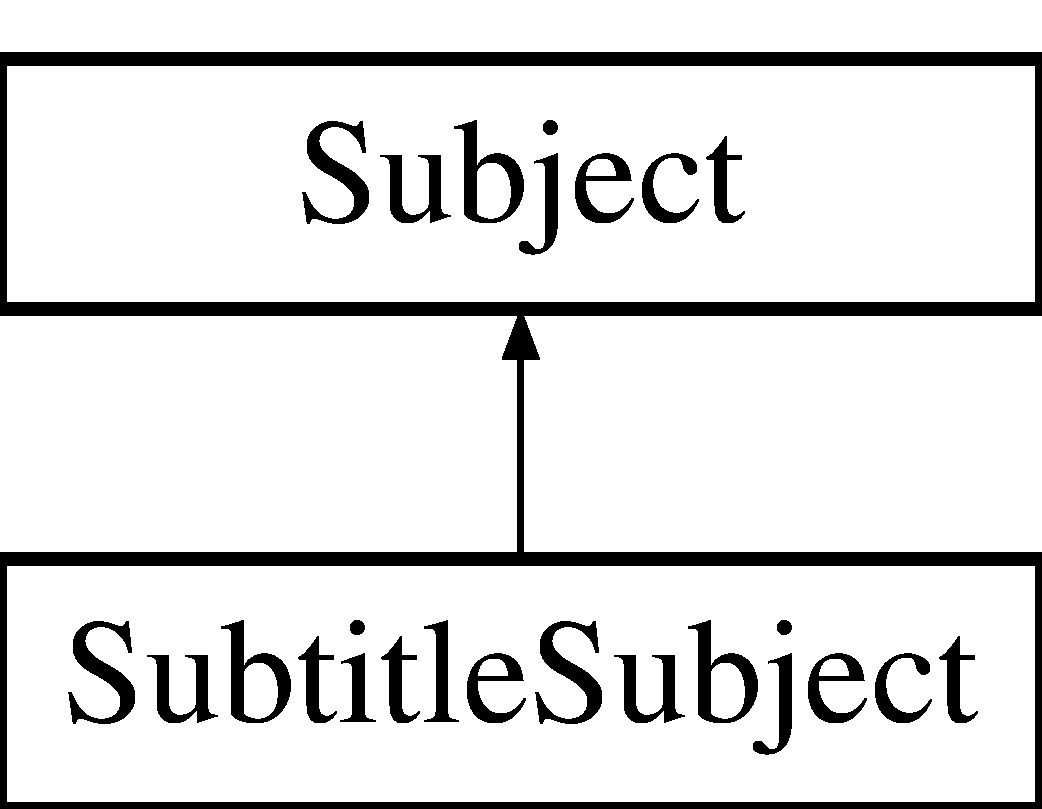
\includegraphics[height=2.000000cm]{classSubtitleSubject}
\end{center}
\end{figure}
\subsection*{Fonctions membres publiques}
\begin{DoxyCompactItemize}
\item 
\hypertarget{classSubtitleSubject_af4cc18f5f05474102ec8ee78649fa42c}{{\bfseries Subtitle\+Subject} (sfe\+::\+Movie $\ast$m)}\label{classSubtitleSubject_af4cc18f5f05474102ec8ee78649fa42c}

\item 
\hypertarget{classSubtitleSubject_afcb35a1af34b6b926860d544893ae3c4}{std\+::string {\bfseries get\+Data} ()}\label{classSubtitleSubject_afcb35a1af34b6b926860d544893ae3c4}

\item 
\hypertarget{classSubtitleSubject_aa6b5f86666e26cb2ed6e3a282f7d9ded}{void {\bfseries set\+Data} (std\+::string l)}\label{classSubtitleSubject_aa6b5f86666e26cb2ed6e3a282f7d9ded}

\item 
\hypertarget{classSubtitleSubject_afc89e947aab454357dce8ea2f80403ee}{int {\bfseries add\+Obs} (\hyperlink{classObserver}{Observer} $\ast$o)}\label{classSubtitleSubject_afc89e947aab454357dce8ea2f80403ee}

\item 
\hypertarget{classSubtitleSubject_a60e75a2a34275176aaea81738ee4879d}{int {\bfseries remove\+Obs} (\hyperlink{classObserver}{Observer} $\ast$o)}\label{classSubtitleSubject_a60e75a2a34275176aaea81738ee4879d}

\item 
\hypertarget{classSubtitleSubject_a25a62553e49435e7ff42ded01d825b52}{void {\bfseries notify\+Obs} ()}\label{classSubtitleSubject_a25a62553e49435e7ff42ded01d825b52}

\item 
\hypertarget{classSubtitleSubject_acd31f06174b7b2a984c9b20566d412b8}{void {\bfseries float\+To\+String} (float i)}\label{classSubtitleSubject_acd31f06174b7b2a984c9b20566d412b8}

\item 
\hypertarget{classSubtitleSubject_a2d774cd5676e57a53b1f9927de5b9b48}{float {\bfseries string\+To\+Float} (std\+::string t)}\label{classSubtitleSubject_a2d774cd5676e57a53b1f9927de5b9b48}

\item 
\hypertarget{classSubtitleSubject_a4a3626c6f2d2f4d4ca6275db6355d1fa}{bool {\bfseries is\+Digit} (std\+::string s)}\label{classSubtitleSubject_a4a3626c6f2d2f4d4ca6275db6355d1fa}

\end{DoxyCompactItemize}


\subsection{Description détaillée}


Définition à la ligne 16 du fichier Subtitle\+Subject.\+hpp.



La documentation de cette classe a été générée à partir du fichier suivant \+:\begin{DoxyCompactItemize}
\item 
src/\+Observer/\hyperlink{SubtitleSubject_8hpp}{Subtitle\+Subject.\+hpp}\end{DoxyCompactItemize}

\hypertarget{classVideo}{\section{Référence de la classe Video}
\label{classVideo}\index{Video@{Video}}
}
\subsection*{Fonctions membres publiques}
\begin{DoxyCompactItemize}
\item 
\hyperlink{classVideo_a54f940a5f19f6bf69ea67fdf62ec8b9c}{Video} (\hyperlink{classVideoInterfaceFactory}{Video\+Interface\+Factory} $\ast$vi\+Fact)
\begin{DoxyCompactList}\small\item\em Constructeur. \end{DoxyCompactList}\item 
\hypertarget{classVideo_aebf7e2a8fa2bbd79335b1cf35925d190}{\hyperlink{classVideo_aebf7e2a8fa2bbd79335b1cf35925d190}{$\sim$\+Video} ()}\label{classVideo_aebf7e2a8fa2bbd79335b1cf35925d190}

\begin{DoxyCompactList}\small\item\em Destructeur. \end{DoxyCompactList}\item 
\hypertarget{classVideo_a787b7cb0faa1c1879b8709247c1efff9}{void \hyperlink{classVideo_a787b7cb0faa1c1879b8709247c1efff9}{afficher} ()}\label{classVideo_a787b7cb0faa1c1879b8709247c1efff9}

\begin{DoxyCompactList}\small\item\em fonction de test de création \end{DoxyCompactList}\item 
\hypertarget{classVideo_a88d85260aae83f3a57c5ead9eda23b6b}{void \hyperlink{classVideo_a88d85260aae83f3a57c5ead9eda23b6b}{run} ()}\label{classVideo_a88d85260aae83f3a57c5ead9eda23b6b}

\begin{DoxyCompactList}\small\item\em lance la vidéo et permet a l'utilisateur d'effectuer des actions dessus. \end{DoxyCompactList}\item 
\hypertarget{classVideo_a5255a0a2f36b0152e9065743a54fadec}{\hyperlink{classEtatV}{Etat\+V} $\ast$ {\bfseries get\+Etat\+Courant} ()}\label{classVideo_a5255a0a2f36b0152e9065743a54fadec}

\item 
\hyperlink{classEtatLectureV}{Etat\+Lecture\+V} $\ast$ \hyperlink{classVideo_aee3ef41850206dac939f736e5b97c73c}{get\+Etat\+Lecture} ()
\begin{DoxyCompactList}\small\item\em Accesseur Etat\+Lecture. \end{DoxyCompactList}\item 
\hyperlink{classEtatPauseV}{Etat\+Pause\+V} $\ast$ \hyperlink{classVideo_a91f40f05211f5b45e772d8bf68de7562}{get\+Etat\+Pause} ()
\begin{DoxyCompactList}\small\item\em Accesseur Etat\+Pause. \end{DoxyCompactList}\item 
\hyperlink{classEtatArretV}{Etat\+Arret\+V} $\ast$ \hyperlink{classVideo_a84d7495527cd76e6347bf85b2ec6e0ab}{get\+Etat\+Arret} ()
\begin{DoxyCompactList}\small\item\em Accesseur Etat\+Arret. \end{DoxyCompactList}\item 
void \hyperlink{classVideo_a515d17189869141a80223055997179c5}{set\+Etat} (\hyperlink{classEtatV}{Etat\+V} $\ast$ev)
\begin{DoxyCompactList}\small\item\em Mutateur Etat. \end{DoxyCompactList}\item 
\hypertarget{classVideo_a8d3ea9525063ce97483e813e11ce4a6a}{void \hyperlink{classVideo_a8d3ea9525063ce97483e813e11ce4a6a}{utiliser\+Bouton\+Lecture} (sfe\+::\+Movie $\ast$movie)}\label{classVideo_a8d3ea9525063ce97483e813e11ce4a6a}

\begin{DoxyCompactList}\small\item\em selon l'état passe la video dans l'état lecture \end{DoxyCompactList}\item 
\hypertarget{classVideo_a93e76d0b95693e0000035e52775bd6d4}{void \hyperlink{classVideo_a93e76d0b95693e0000035e52775bd6d4}{utiliser\+Bouton\+Stop} (sfe\+::\+Movie $\ast$movie)}\label{classVideo_a93e76d0b95693e0000035e52775bd6d4}

\begin{DoxyCompactList}\small\item\em selon l'etat, effectue l'action du bouttonstop \end{DoxyCompactList}\item 
\hypertarget{classVideo_a78f816a4576618435c101756a96daea0}{void \hyperlink{classVideo_a78f816a4576618435c101756a96daea0}{utiliser\+Bouton\+Pause} (sfe\+::\+Movie $\ast$movie)}\label{classVideo_a78f816a4576618435c101756a96daea0}

\begin{DoxyCompactList}\small\item\em selon l'etat, effectue l'action du bouttonpause \end{DoxyCompactList}\end{DoxyCompactItemize}


\subsection{Description détaillée}


Définition à la ligne 10 du fichier video.\+hpp.



\subsection{Documentation des constructeurs et destructeur}
\hypertarget{classVideo_a54f940a5f19f6bf69ea67fdf62ec8b9c}{\index{Video@{Video}!Video@{Video}}
\index{Video@{Video}!Video@{Video}}
\subsubsection[{Video}]{\setlength{\rightskip}{0pt plus 5cm}Video\+::\+Video (
\begin{DoxyParamCaption}
\item[{{\bf Video\+Interface\+Factory} $\ast$}]{vi\+Fact}
\end{DoxyParamCaption}
)}}\label{classVideo_a54f940a5f19f6bf69ea67fdf62ec8b9c}


Constructeur. 


\begin{DoxyParams}{Paramètres}
{\em Video\+Interface\+Factory$\ast$} & vi\+Fact \+: factory de l'interface video \\
\hline
\end{DoxyParams}


\subsection{Documentation des fonctions membres}
\hypertarget{classVideo_a84d7495527cd76e6347bf85b2ec6e0ab}{\index{Video@{Video}!get\+Etat\+Arret@{get\+Etat\+Arret}}
\index{get\+Etat\+Arret@{get\+Etat\+Arret}!Video@{Video}}
\subsubsection[{get\+Etat\+Arret}]{\setlength{\rightskip}{0pt plus 5cm}{\bf Etat\+Arret\+V}$\ast$ Video\+::get\+Etat\+Arret (
\begin{DoxyParamCaption}
{}
\end{DoxyParamCaption}
)}}\label{classVideo_a84d7495527cd76e6347bf85b2ec6e0ab}


Accesseur Etat\+Arret. 

\begin{DoxyReturn}{Renvoie}
\hyperlink{classEtatArretV}{Etat\+Arret\+V} \+: pointeur sur l'état arret de la video 
\end{DoxyReturn}
\hypertarget{classVideo_aee3ef41850206dac939f736e5b97c73c}{\index{Video@{Video}!get\+Etat\+Lecture@{get\+Etat\+Lecture}}
\index{get\+Etat\+Lecture@{get\+Etat\+Lecture}!Video@{Video}}
\subsubsection[{get\+Etat\+Lecture}]{\setlength{\rightskip}{0pt plus 5cm}{\bf Etat\+Lecture\+V}$\ast$ Video\+::get\+Etat\+Lecture (
\begin{DoxyParamCaption}
{}
\end{DoxyParamCaption}
)}}\label{classVideo_aee3ef41850206dac939f736e5b97c73c}


Accesseur Etat\+Lecture. 

\begin{DoxyReturn}{Renvoie}
Etat\+Lecture\+V\+A$\ast$ \+: pointeur sur l'état lecture de la vidéo 
\end{DoxyReturn}
\hypertarget{classVideo_a91f40f05211f5b45e772d8bf68de7562}{\index{Video@{Video}!get\+Etat\+Pause@{get\+Etat\+Pause}}
\index{get\+Etat\+Pause@{get\+Etat\+Pause}!Video@{Video}}
\subsubsection[{get\+Etat\+Pause}]{\setlength{\rightskip}{0pt plus 5cm}{\bf Etat\+Pause\+V}$\ast$ Video\+::get\+Etat\+Pause (
\begin{DoxyParamCaption}
{}
\end{DoxyParamCaption}
)}}\label{classVideo_a91f40f05211f5b45e772d8bf68de7562}


Accesseur Etat\+Pause. 

\begin{DoxyReturn}{Renvoie}
Etat\+Pause\+V$\ast$ \+: pointeur sur l'état pause de la vidéo 
\end{DoxyReturn}
\hypertarget{classVideo_a515d17189869141a80223055997179c5}{\index{Video@{Video}!set\+Etat@{set\+Etat}}
\index{set\+Etat@{set\+Etat}!Video@{Video}}
\subsubsection[{set\+Etat}]{\setlength{\rightskip}{0pt plus 5cm}void Video\+::set\+Etat (
\begin{DoxyParamCaption}
\item[{{\bf Etat\+V} $\ast$}]{ev}
\end{DoxyParamCaption}
)}}\label{classVideo_a515d17189869141a80223055997179c5}


Mutateur Etat. 


\begin{DoxyParams}{Paramètres}
{\em \hyperlink{classEtatV}{Etat\+V}} & ev \+: le nouvel etat de l'audio \\
\hline
\end{DoxyParams}


La documentation de cette classe a été générée à partir du fichier suivant \+:\begin{DoxyCompactItemize}
\item 
src/video.\+hpp\end{DoxyCompactItemize}

\hypertarget{classVideoInterfaceFactory}{\section{Référence de la classe Video\+Interface\+Factory}
\label{classVideoInterfaceFactory}\index{Video\+Interface\+Factory@{Video\+Interface\+Factory}}
}
Graphe d'héritage de Video\+Interface\+Factory\+:\begin{figure}[H]
\begin{center}
\leavevmode
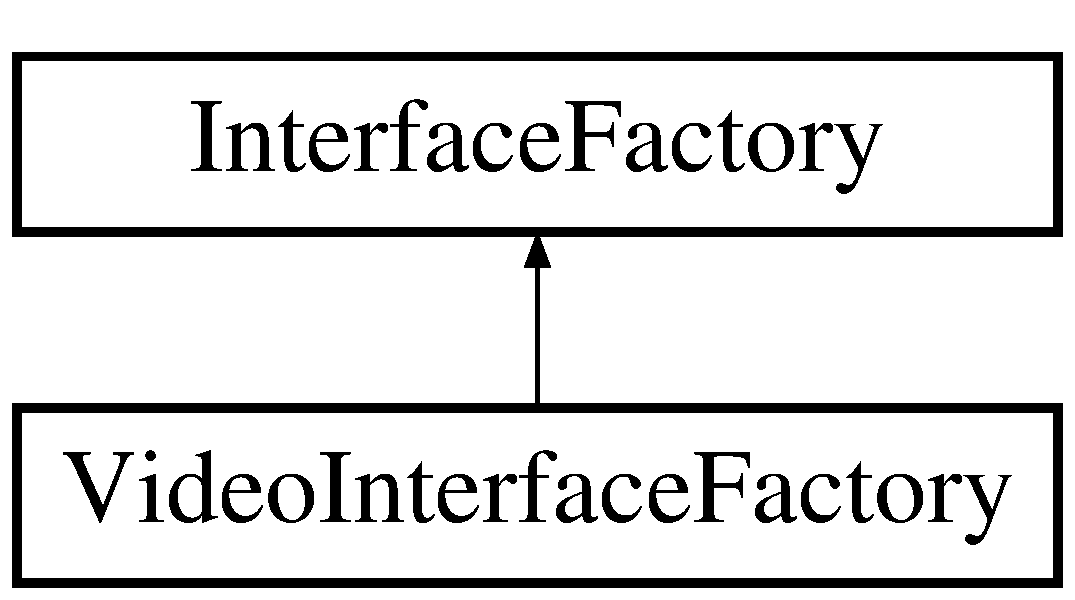
\includegraphics[height=2.000000cm]{classVideoInterfaceFactory}
\end{center}
\end{figure}
\subsection*{Fonctions membres publiques}
\begin{DoxyCompactItemize}
\item 
\hyperlink{classInterface}{Interface} \hyperlink{classVideoInterfaceFactory_ac0470dfd9d2685893c62ec922496a9bf}{create\+Interface} (\hyperlink{classButtons}{Buttons} $\ast$b, \hyperlink{classFormat}{Format} $\ast$f)
\begin{DoxyCompactList}\small\item\em Crée l'interface adéquate à la lecture d'un fichier video. \end{DoxyCompactList}\end{DoxyCompactItemize}


\subsection{Description détaillée}


Définition à la ligne 16 du fichier video\+Interface\+Factory.\+hpp.



\subsection{Documentation des fonctions membres}
\hypertarget{classVideoInterfaceFactory_ac0470dfd9d2685893c62ec922496a9bf}{\index{Video\+Interface\+Factory@{Video\+Interface\+Factory}!create\+Interface@{create\+Interface}}
\index{create\+Interface@{create\+Interface}!Video\+Interface\+Factory@{Video\+Interface\+Factory}}
\subsubsection[{create\+Interface}]{\setlength{\rightskip}{0pt plus 5cm}{\bf Interface} Video\+Interface\+Factory\+::create\+Interface (
\begin{DoxyParamCaption}
\item[{{\bf Buttons} $\ast$}]{b, }
\item[{{\bf Format} $\ast$}]{f}
\end{DoxyParamCaption}
)\hspace{0.3cm}{\ttfamily [virtual]}}}\label{classVideoInterfaceFactory_ac0470dfd9d2685893c62ec922496a9bf}


Crée l'interface adéquate à la lecture d'un fichier video. 


\begin{DoxyParams}{Paramètres}
{\em Buttons\+Va} & bva, \hyperlink{classFormatBig}{Format\+Big} fb \\
\hline
\end{DoxyParams}


Implémente \hyperlink{classInterfaceFactory_a043c593647071e277c897a5416221de0}{Interface\+Factory}.



La documentation de cette classe a été générée à partir du fichier suivant \+:\begin{DoxyCompactItemize}
\item 
src/\+Abstract\+Factory/\hyperlink{videoInterfaceFactory_8hpp}{video\+Interface\+Factory.\+hpp}\end{DoxyCompactItemize}

\chapter{Documentation des fichiers}
\hypertarget{audioInterfaceFactory_8hpp}{\section{Référence du fichier src/\+Abstract\+Factory/audio\+Interface\+Factory.hpp}
\label{audioInterfaceFactory_8hpp}\index{src/\+Abstract\+Factory/audio\+Interface\+Factory.\+hpp@{src/\+Abstract\+Factory/audio\+Interface\+Factory.\+hpp}}
}


Classe \hyperlink{classAudioInterfaceFactory}{Audio\+Interface\+Factory}, utilisé pour la création de l'interface lors de la lecture d'un fichier audio.  


{\ttfamily \#include \char`\"{}interface\+Factory.\+hpp\char`\"{}}\\*
{\ttfamily \#include \char`\"{}interface.\+hpp\char`\"{}}\\*
{\ttfamily \#include \char`\"{}buttons\+V\+A.\+hpp\char`\"{}}\\*
{\ttfamily \#include \char`\"{}format\+Small.\+hpp\char`\"{}}\\*
\subsection*{Classes}
\begin{DoxyCompactItemize}
\item 
class \hyperlink{classAudioInterfaceFactory}{Audio\+Interface\+Factory}
\end{DoxyCompactItemize}


\subsection{Description détaillée}
Classe \hyperlink{classAudioInterfaceFactory}{Audio\+Interface\+Factory}, utilisé pour la création de l'interface lors de la lecture d'un fichier audio. 

\begin{DoxyAuthor}{Auteur}
K.\+Gomes / K.\+Espasa 
\end{DoxyAuthor}


Définition dans le fichier \hyperlink{audioInterfaceFactory_8hpp_source}{audio\+Interface\+Factory.\+hpp}.


\hypertarget{buttons_8hpp}{\section{Référence du fichier src/\+Abstract\+Factory/buttons.hpp}
\label{buttons_8hpp}\index{src/\+Abstract\+Factory/buttons.\+hpp@{src/\+Abstract\+Factory/buttons.\+hpp}}
}


\hyperlink{classInterface}{Interface} \hyperlink{classButtons}{Buttons}, permettant de créer les boutons adéquats selon le type de média.  


{\ttfamily \#include $<$S\+F\+M\+L/\+Graphics.\+hpp$>$}\\*
{\ttfamily \#include $<$T\+G\+U\+I/\+T\+G\+U\+I.\+hpp$>$}\\*
\subsection*{Classes}
\begin{DoxyCompactItemize}
\item 
class \hyperlink{classButtons}{Buttons}
\end{DoxyCompactItemize}


\subsection{Description détaillée}
\hyperlink{classInterface}{Interface} \hyperlink{classButtons}{Buttons}, permettant de créer les boutons adéquats selon le type de média. 

\begin{DoxyAuthor}{Auteur}
K.\+Gomes / K.\+Espasa 
\end{DoxyAuthor}


Définition dans le fichier \hyperlink{buttons_8hpp_source}{buttons.\+hpp}.


\hypertarget{buttonsI_8hpp}{\section{Référence du fichier src/\+Abstract\+Factory/buttons\+I.hpp}
\label{buttonsI_8hpp}\index{src/\+Abstract\+Factory/buttons\+I.\+hpp@{src/\+Abstract\+Factory/buttons\+I.\+hpp}}
}


Classe \hyperlink{classButtonsI}{Buttons\+I}, héritant de \hyperlink{classButtons}{Buttons}, permettant de créer les boutons \char`\"{}image\char`\"{} nécessaire dans une interface.  


{\ttfamily \#include \char`\"{}buttons.\+hpp\char`\"{}}\\*
{\ttfamily \#include $<$S\+F\+M\+L/\+Graphics.\+hpp$>$}\\*
{\ttfamily \#include $<$T\+G\+U\+I/\+T\+G\+U\+I.\+hpp$>$}\\*
\subsection*{Classes}
\begin{DoxyCompactItemize}
\item 
class \hyperlink{classButtonsI}{Buttons\+I}
\end{DoxyCompactItemize}


\subsection{Description détaillée}
Classe \hyperlink{classButtonsI}{Buttons\+I}, héritant de \hyperlink{classButtons}{Buttons}, permettant de créer les boutons \char`\"{}image\char`\"{} nécessaire dans une interface. 

\begin{DoxyAuthor}{Auteur}
K.\+Gomes / K.\+Espasa 
\end{DoxyAuthor}


Définition dans le fichier \hyperlink{buttonsI_8hpp_source}{buttons\+I.\+hpp}.


\hypertarget{buttonsVA_8hpp}{\section{Référence du fichier src/\+Abstract\+Factory/buttons\+V\+A.hpp}
\label{buttonsVA_8hpp}\index{src/\+Abstract\+Factory/buttons\+V\+A.\+hpp@{src/\+Abstract\+Factory/buttons\+V\+A.\+hpp}}
}


Classe \hyperlink{classButtonsVA}{Buttons\+V\+A}, permettant de créer les boutons de type \char`\"{}video / audio\char`\"{} nécessaires dans une interface.  


{\ttfamily \#include \char`\"{}buttons.\+hpp\char`\"{}}\\*
{\ttfamily \#include $<$S\+F\+M\+L/\+Graphics.\+hpp$>$}\\*
{\ttfamily \#include $<$T\+G\+U\+I/\+T\+G\+U\+I.\+hpp$>$}\\*
\subsection*{Classes}
\begin{DoxyCompactItemize}
\item 
class \hyperlink{classButtonsVA}{Buttons\+V\+A}
\end{DoxyCompactItemize}


\subsection{Description détaillée}
Classe \hyperlink{classButtonsVA}{Buttons\+V\+A}, permettant de créer les boutons de type \char`\"{}video / audio\char`\"{} nécessaires dans une interface. 

\begin{DoxyAuthor}{Auteur}
K.\+Gomes / K.\+Espasa 
\end{DoxyAuthor}


Définition dans le fichier \hyperlink{buttonsVA_8hpp_source}{buttons\+V\+A.\+hpp}.


\hypertarget{format_8hpp}{\section{Référence du fichier src/\+Abstract\+Factory/format.hpp}
\label{format_8hpp}\index{src/\+Abstract\+Factory/format.\+hpp@{src/\+Abstract\+Factory/format.\+hpp}}
}


\hyperlink{classInterface}{Interface} \hyperlink{classFormat}{Format}, permettant de créer le format adéquat selon le type de média.  


{\ttfamily \#include $<$S\+F\+M\+L/\+Graphics.\+hpp$>$}\\*
{\ttfamily \#include $<$T\+G\+U\+I/\+T\+G\+U\+I.\+hpp$>$}\\*
\subsection*{Classes}
\begin{DoxyCompactItemize}
\item 
class \hyperlink{classFormat}{Format}
\end{DoxyCompactItemize}


\subsection{Description détaillée}
\hyperlink{classInterface}{Interface} \hyperlink{classFormat}{Format}, permettant de créer le format adéquat selon le type de média. 

\begin{DoxyAuthor}{Auteur}
K.\+Gomes / K.\+Espasa 
\end{DoxyAuthor}


Définition dans le fichier \hyperlink{format_8hpp_source}{format.\+hpp}.


\hypertarget{formatBig_8hpp}{\section{Référence du fichier src/\+Abstract\+Factory/format\+Big.hpp}
\label{formatBig_8hpp}\index{src/\+Abstract\+Factory/format\+Big.\+hpp@{src/\+Abstract\+Factory/format\+Big.\+hpp}}
}


Classe \hyperlink{classFormatBig}{Format\+Big}, permettant de créer le format \char`\"{}grand\char`\"{}.  


{\ttfamily \#include \char`\"{}format.\+hpp\char`\"{}}\\*
\subsection*{Classes}
\begin{DoxyCompactItemize}
\item 
class \hyperlink{classFormatBig}{Format\+Big}
\end{DoxyCompactItemize}


\subsection{Description détaillée}
Classe \hyperlink{classFormatBig}{Format\+Big}, permettant de créer le format \char`\"{}grand\char`\"{}. 

\begin{DoxyAuthor}{Auteur}
K.\+Gomes / K.\+Espasa 
\end{DoxyAuthor}


Définition dans le fichier \hyperlink{formatBig_8hpp_source}{format\+Big.\+hpp}.


\hypertarget{formatSmall_8hpp}{\section{Référence du fichier src/\+Abstract\+Factory/format\+Small.hpp}
\label{formatSmall_8hpp}\index{src/\+Abstract\+Factory/format\+Small.\+hpp@{src/\+Abstract\+Factory/format\+Small.\+hpp}}
}


Classe \hyperlink{classFormatSmall}{Format\+Small}, permettant de créer le format \char`\"{}petit\char`\"{}.  


{\ttfamily \#include \char`\"{}format.\+hpp\char`\"{}}\\*
\subsection*{Classes}
\begin{DoxyCompactItemize}
\item 
class \hyperlink{classFormatSmall}{Format\+Small}
\end{DoxyCompactItemize}


\subsection{Description détaillée}
Classe \hyperlink{classFormatSmall}{Format\+Small}, permettant de créer le format \char`\"{}petit\char`\"{}. 

\begin{DoxyAuthor}{Auteur}
K.\+Gomes / K.\+Espasa 
\end{DoxyAuthor}


Définition dans le fichier \hyperlink{formatSmall_8hpp_source}{format\+Small.\+hpp}.


\hypertarget{imageInterfaceFactory_8hpp}{\section{Référence du fichier src/\+Abstract\+Factory/image\+Interface\+Factory.hpp}
\label{imageInterfaceFactory_8hpp}\index{src/\+Abstract\+Factory/image\+Interface\+Factory.\+hpp@{src/\+Abstract\+Factory/image\+Interface\+Factory.\+hpp}}
}


Classe \hyperlink{classImageInterfaceFactory}{Image\+Interface\+Factory}, utilisé pour la création de l'interface lors de la lecture d'un fichier image.  


{\ttfamily \#include \char`\"{}interface\+Factory.\+hpp\char`\"{}}\\*
{\ttfamily \#include \char`\"{}interface.\+hpp\char`\"{}}\\*
{\ttfamily \#include \char`\"{}buttons\+I.\+hpp\char`\"{}}\\*
{\ttfamily \#include \char`\"{}format\+Big.\+hpp\char`\"{}}\\*
\subsection*{Classes}
\begin{DoxyCompactItemize}
\item 
class \hyperlink{classImageInterfaceFactory}{Image\+Interface\+Factory}
\end{DoxyCompactItemize}


\subsection{Description détaillée}
Classe \hyperlink{classImageInterfaceFactory}{Image\+Interface\+Factory}, utilisé pour la création de l'interface lors de la lecture d'un fichier image. 

\begin{DoxyAuthor}{Auteur}
K.\+Gomes / K.\+Espasa 
\end{DoxyAuthor}


Définition dans le fichier \hyperlink{imageInterfaceFactory_8hpp_source}{image\+Interface\+Factory.\+hpp}.


\hypertarget{interface_8hpp}{\section{Référence du fichier src/\+Abstract\+Factory/interface.hpp}
\label{interface_8hpp}\index{src/\+Abstract\+Factory/interface.\+hpp@{src/\+Abstract\+Factory/interface.\+hpp}}
}


Classe \hyperlink{classInterface}{Interface}.  


{\ttfamily \#include $<$vector$>$}\\*
{\ttfamily \#include \char`\"{}format.\+hpp\char`\"{}}\\*
{\ttfamily \#include \char`\"{}buttons.\+hpp\char`\"{}}\\*
{\ttfamily \#include $<$S\+F\+M\+L/\+Graphics.\+hpp$>$}\\*
{\ttfamily \#include $<$T\+G\+U\+I/\+T\+G\+U\+I.\+hpp$>$}\\*
\subsection*{Classes}
\begin{DoxyCompactItemize}
\item 
class \hyperlink{classInterface}{Interface}
\end{DoxyCompactItemize}


\subsection{Description détaillée}
Classe \hyperlink{classInterface}{Interface}. 

\begin{DoxyAuthor}{Auteur}
K.\+Gomes / K.\+Espasa 
\end{DoxyAuthor}


Définition dans le fichier \hyperlink{interface_8hpp_source}{interface.\+hpp}.


\hypertarget{interfaceFactory_8hpp}{\section{Référence du fichier src/\+Abstract\+Factory/interface\+Factory.hpp}
\label{interfaceFactory_8hpp}\index{src/\+Abstract\+Factory/interface\+Factory.\+hpp@{src/\+Abstract\+Factory/interface\+Factory.\+hpp}}
}


Classe \hyperlink{classInterfaceFactory}{Interface\+Factory}, permettant de créer l'interface adéquate selon le type de média.  


{\ttfamily \#include \char`\"{}interface.\+hpp\char`\"{}}\\*
\subsection*{Classes}
\begin{DoxyCompactItemize}
\item 
class \hyperlink{classInterfaceFactory}{Interface\+Factory}
\end{DoxyCompactItemize}


\subsection{Description détaillée}
Classe \hyperlink{classInterfaceFactory}{Interface\+Factory}, permettant de créer l'interface adéquate selon le type de média. 

\begin{DoxyAuthor}{Auteur}
K.\+Gomes / K.\+Espasa 
\end{DoxyAuthor}


Définition dans le fichier \hyperlink{interfaceFactory_8hpp_source}{interface\+Factory.\+hpp}.


\hypertarget{videoInterfaceFactory_8hpp}{\section{Référence du fichier src/\+Abstract\+Factory/video\+Interface\+Factory.hpp}
\label{videoInterfaceFactory_8hpp}\index{src/\+Abstract\+Factory/video\+Interface\+Factory.\+hpp@{src/\+Abstract\+Factory/video\+Interface\+Factory.\+hpp}}
}


Classe \hyperlink{classVideoInterfaceFactory}{Video\+Interface\+Factory}, utilisé pour la création de l'interface lors de la lecture d'un fichier video.  


{\ttfamily \#include \char`\"{}interface\+Factory.\+hpp\char`\"{}}\\*
{\ttfamily \#include \char`\"{}interface.\+hpp\char`\"{}}\\*
{\ttfamily \#include \char`\"{}buttons\+V\+A.\+hpp\char`\"{}}\\*
{\ttfamily \#include \char`\"{}format\+Big.\+hpp\char`\"{}}\\*
\subsection*{Classes}
\begin{DoxyCompactItemize}
\item 
class \hyperlink{classVideoInterfaceFactory}{Video\+Interface\+Factory}
\end{DoxyCompactItemize}


\subsection{Description détaillée}
Classe \hyperlink{classVideoInterfaceFactory}{Video\+Interface\+Factory}, utilisé pour la création de l'interface lors de la lecture d'un fichier video. 

\begin{DoxyAuthor}{Auteur}
K.\+Gomes / K.\+Espasa 
\end{DoxyAuthor}


Définition dans le fichier \hyperlink{videoInterfaceFactory_8hpp_source}{video\+Interface\+Factory.\+hpp}.


\hypertarget{Dir_8hpp}{\section{Référence du fichier src/\+Dir/\+Dir.hpp}
\label{Dir_8hpp}\index{src/\+Dir/\+Dir.\+hpp@{src/\+Dir/\+Dir.\+hpp}}
}


Classe \hyperlink{classDir}{Dir} , contenant les méthodes pour acceder aux fichiers d'un dossier et les stockants.  


{\ttfamily \#include $<$vector$>$}\\*
{\ttfamily \#include $<$string$>$}\\*
{\ttfamily \#include $<$T\+G\+U\+I/\+T\+G\+U\+I.\+hpp$>$}\\*
{\ttfamily \#include $<$boost/filesystem.\+hpp$>$}\\*
{\ttfamily \#include $<$boost/range/iterator\+\_\+range.\+hpp$>$}\\*
\subsection*{Classes}
\begin{DoxyCompactItemize}
\item 
class \hyperlink{classDir}{Dir}
\end{DoxyCompactItemize}


\subsection{Description détaillée}
Classe \hyperlink{classDir}{Dir} , contenant les méthodes pour acceder aux fichiers d'un dossier et les stockants. 

\begin{DoxyAuthor}{Auteur}
K.\+Gomes / K.\+Espasa 
\end{DoxyAuthor}


Définition dans le fichier \hyperlink{Dir_8hpp_source}{Dir.\+hpp}.


\hypertarget{Observer_8hpp}{\section{Référence du fichier src/\+Observer/\+Observer.hpp}
\label{Observer_8hpp}\index{src/\+Observer/\+Observer.\+hpp@{src/\+Observer/\+Observer.\+hpp}}
}


Classe \hyperlink{classObserver}{Observer} (abstract)  


{\ttfamily \#include $<$iostream$>$}\\*
{\ttfamily \#include \char`\"{}Subject.\+hpp\char`\"{}}\\*
\subsection*{Classes}
\begin{DoxyCompactItemize}
\item 
class \hyperlink{classObserver}{Observer}
\end{DoxyCompactItemize}


\subsection{Description détaillée}
Classe \hyperlink{classObserver}{Observer} (abstract) 

\begin{DoxyAuthor}{Auteur}
K.\+Gomes / K.\+Espasa 
\end{DoxyAuthor}


Définition dans le fichier \hyperlink{Observer_8hpp_source}{Observer.\+hpp}.


\hypertarget{SubtitleLineObs_8hpp}{\section{Référence du fichier src/\+Observer/\+Subtitle\+Line\+Obs.hpp}
\label{SubtitleLineObs_8hpp}\index{src/\+Observer/\+Subtitle\+Line\+Obs.\+hpp@{src/\+Observer/\+Subtitle\+Line\+Obs.\+hpp}}
}


Classe \hyperlink{classSubtitleLineObs}{Subtitle\+Line\+Obs} , contenant les méthodes pour l'observeur.  


{\ttfamily \#include \char`\"{}Observer.\+hpp\char`\"{}}\\*
{\ttfamily \#include $<$T\+G\+U\+I/\+T\+G\+U\+I.\+hpp$>$}\\*
\subsection*{Classes}
\begin{DoxyCompactItemize}
\item 
class \hyperlink{classSubtitleLineObs}{Subtitle\+Line\+Obs}
\end{DoxyCompactItemize}


\subsection{Description détaillée}
Classe \hyperlink{classSubtitleLineObs}{Subtitle\+Line\+Obs} , contenant les méthodes pour l'observeur. 

\begin{DoxyAuthor}{Auteur}
K.\+Gomes / K.\+Espasa 
\end{DoxyAuthor}


Définition dans le fichier \hyperlink{SubtitleLineObs_8hpp_source}{Subtitle\+Line\+Obs.\+hpp}.


\hypertarget{SubtitleSubject_8hpp}{\section{Référence du fichier src/\+Observer/\+Subtitle\+Subject.hpp}
\label{SubtitleSubject_8hpp}\index{src/\+Observer/\+Subtitle\+Subject.\+hpp@{src/\+Observer/\+Subtitle\+Subject.\+hpp}}
}


Classe \hyperlink{classSubtitleSubject}{Subtitle\+Subject} , contenant les méthodes du sujet à observer.  


{\ttfamily \#include \char`\"{}Subject.\+hpp\char`\"{}}\\*
{\ttfamily \#include $<$sfe\+Movie/\+Movie.\+hpp$>$}\\*
{\ttfamily \#include $<$vector$>$}\\*
{\ttfamily \#include $<$ctime$>$}\\*
\subsection*{Classes}
\begin{DoxyCompactItemize}
\item 
class \hyperlink{classSubtitleSubject}{Subtitle\+Subject}
\end{DoxyCompactItemize}


\subsection{Description détaillée}
Classe \hyperlink{classSubtitleSubject}{Subtitle\+Subject} , contenant les méthodes du sujet à observer. 

\begin{DoxyAuthor}{Auteur}
K.\+Gomes / K.\+Espasa 
\end{DoxyAuthor}


Définition dans le fichier \hyperlink{SubtitleSubject_8hpp_source}{Subtitle\+Subject.\+hpp}.


\hypertarget{etatA_8hpp}{\section{Référence du fichier src/\+State\+Audio/etat\+A.hpp}
\label{etatA_8hpp}\index{src/\+State\+Audio/etat\+A.\+hpp@{src/\+State\+Audio/etat\+A.\+hpp}}
}


Classe \hyperlink{classEtatA}{Etat\+A} (abstraite), contenant les méthodes applicables à un audio.  


{\ttfamily \#include $<$S\+F\+M\+L/\+Audio.\+hpp$>$}\\*
{\ttfamily \#include $<$iostream$>$}\\*
\subsection*{Classes}
\begin{DoxyCompactItemize}
\item 
class \hyperlink{classEtatA}{Etat\+A}
\end{DoxyCompactItemize}


\subsection{Description détaillée}
Classe \hyperlink{classEtatA}{Etat\+A} (abstraite), contenant les méthodes applicables à un audio. 

\begin{DoxyAuthor}{Auteur}
K.\+Gomes / K.\+Espasa 
\end{DoxyAuthor}


Définition dans le fichier \hyperlink{etatA_8hpp_source}{etat\+A.\+hpp}.


\hypertarget{etatArretA_8hpp}{\section{Référence du fichier src/\+State\+Audio/etat\+Arret\+A.hpp}
\label{etatArretA_8hpp}\index{src/\+State\+Audio/etat\+Arret\+A.\+hpp@{src/\+State\+Audio/etat\+Arret\+A.\+hpp}}
}


Classe \hyperlink{classEtatArretA}{Etat\+Arret\+A}, qui implémente les méthodes applicables à un audio dans l'état arret.  


{\ttfamily \#include \char`\"{}etat\+A.\+hpp\char`\"{}}\\*
\subsection*{Classes}
\begin{DoxyCompactItemize}
\item 
class \hyperlink{classEtatArretA}{Etat\+Arret\+A}
\end{DoxyCompactItemize}


\subsection{Description détaillée}
Classe \hyperlink{classEtatArretA}{Etat\+Arret\+A}, qui implémente les méthodes applicables à un audio dans l'état arret. 

\begin{DoxyAuthor}{Auteur}
K.\+Gomes / K.\+Espasa 
\end{DoxyAuthor}


Définition dans le fichier \hyperlink{etatArretA_8hpp_source}{etat\+Arret\+A.\+hpp}.


\hypertarget{etatLectureA_8hpp}{\section{Référence du fichier src/\+State\+Audio/etat\+Lecture\+A.hpp}
\label{etatLectureA_8hpp}\index{src/\+State\+Audio/etat\+Lecture\+A.\+hpp@{src/\+State\+Audio/etat\+Lecture\+A.\+hpp}}
}


Classe \hyperlink{classEtatLectureA}{Etat\+Lecture\+A}, qui implémente les méthodes applicables à un audio dans l'état lecture.  


{\ttfamily \#include \char`\"{}etat\+A.\+hpp\char`\"{}}\\*
\subsection*{Classes}
\begin{DoxyCompactItemize}
\item 
class \hyperlink{classEtatLectureA}{Etat\+Lecture\+A}
\end{DoxyCompactItemize}


\subsection{Description détaillée}
Classe \hyperlink{classEtatLectureA}{Etat\+Lecture\+A}, qui implémente les méthodes applicables à un audio dans l'état lecture. 

\begin{DoxyAuthor}{Auteur}
K.\+Gomes / K.\+Espasa 
\end{DoxyAuthor}


Définition dans le fichier \hyperlink{etatLectureA_8hpp_source}{etat\+Lecture\+A.\+hpp}.


\hypertarget{etatPauseA_8hpp}{\section{Référence du fichier src/\+State\+Audio/etat\+Pause\+A.hpp}
\label{etatPauseA_8hpp}\index{src/\+State\+Audio/etat\+Pause\+A.\+hpp@{src/\+State\+Audio/etat\+Pause\+A.\+hpp}}
}


Classe \hyperlink{classEtatPauseA}{Etat\+Pause\+A}, qui implémente les méthodes applicables à un audio dans l'état pause.  


{\ttfamily \#include \char`\"{}etat\+A.\+hpp\char`\"{}}\\*
\subsection*{Classes}
\begin{DoxyCompactItemize}
\item 
class \hyperlink{classEtatPauseA}{Etat\+Pause\+A}
\end{DoxyCompactItemize}


\subsection{Description détaillée}
Classe \hyperlink{classEtatPauseA}{Etat\+Pause\+A}, qui implémente les méthodes applicables à un audio dans l'état pause. 

\begin{DoxyAuthor}{Auteur}
K.\+Gomes / K.\+Espasa 
\end{DoxyAuthor}


Définition dans le fichier \hyperlink{etatPauseA_8hpp_source}{etat\+Pause\+A.\+hpp}.


\hypertarget{etatArretV_8hpp}{\section{Référence du fichier src/\+State\+Video/etat\+Arret\+V.hpp}
\label{etatArretV_8hpp}\index{src/\+State\+Video/etat\+Arret\+V.\+hpp@{src/\+State\+Video/etat\+Arret\+V.\+hpp}}
}


Classe \hyperlink{classEtatArretV}{Etat\+Arret\+V}, qui implémente les méthodes applicables à une vidéo dans l'état arret.  


{\ttfamily \#include \char`\"{}etat\+V.\+hpp\char`\"{}}\\*
\subsection*{Classes}
\begin{DoxyCompactItemize}
\item 
class \hyperlink{classEtatArretV}{Etat\+Arret\+V}
\end{DoxyCompactItemize}


\subsection{Description détaillée}
Classe \hyperlink{classEtatArretV}{Etat\+Arret\+V}, qui implémente les méthodes applicables à une vidéo dans l'état arret. 

\begin{DoxyAuthor}{Auteur}
K.\+Gomes / K.\+Espasa 
\end{DoxyAuthor}


Définition dans le fichier \hyperlink{etatArretV_8hpp_source}{etat\+Arret\+V.\+hpp}.


\hypertarget{etatLectureV_8hpp}{\section{Référence du fichier src/\+State\+Video/etat\+Lecture\+V.hpp}
\label{etatLectureV_8hpp}\index{src/\+State\+Video/etat\+Lecture\+V.\+hpp@{src/\+State\+Video/etat\+Lecture\+V.\+hpp}}
}


Classe \hyperlink{classEtatLectureV}{Etat\+Lecture\+V}, qui implémente les méthodes applicables à une vidéo dans l'état lecture.  


{\ttfamily \#include \char`\"{}etat\+V.\+hpp\char`\"{}}\\*
\subsection*{Classes}
\begin{DoxyCompactItemize}
\item 
class \hyperlink{classEtatLectureV}{Etat\+Lecture\+V}
\end{DoxyCompactItemize}


\subsection{Description détaillée}
Classe \hyperlink{classEtatLectureV}{Etat\+Lecture\+V}, qui implémente les méthodes applicables à une vidéo dans l'état lecture. 

\begin{DoxyAuthor}{Auteur}
K.\+Gomes / K.\+Espasa 
\end{DoxyAuthor}


Définition dans le fichier \hyperlink{etatLectureV_8hpp_source}{etat\+Lecture\+V.\+hpp}.


\hypertarget{etatPauseV_8hpp}{\section{Référence du fichier src/\+State\+Video/etat\+Pause\+V.hpp}
\label{etatPauseV_8hpp}\index{src/\+State\+Video/etat\+Pause\+V.\+hpp@{src/\+State\+Video/etat\+Pause\+V.\+hpp}}
}


Classe \hyperlink{classEtatPauseV}{Etat\+Pause\+V}, qui implémente les méthodes applicables à une video dans l'état pause.  


{\ttfamily \#include \char`\"{}etat\+V.\+hpp\char`\"{}}\\*
\subsection*{Classes}
\begin{DoxyCompactItemize}
\item 
class \hyperlink{classEtatPauseV}{Etat\+Pause\+V}
\end{DoxyCompactItemize}


\subsection{Description détaillée}
Classe \hyperlink{classEtatPauseV}{Etat\+Pause\+V}, qui implémente les méthodes applicables à une video dans l'état pause. 

\begin{DoxyAuthor}{Auteur}
K.\+Gomes / K.\+Espasa 
\end{DoxyAuthor}


Définition dans le fichier \hyperlink{etatPauseV_8hpp_source}{etat\+Pause\+V.\+hpp}.


\hypertarget{etatV_8hpp}{\section{Référence du fichier src/\+State\+Video/etat\+V.hpp}
\label{etatV_8hpp}\index{src/\+State\+Video/etat\+V.\+hpp@{src/\+State\+Video/etat\+V.\+hpp}}
}


Classe \hyperlink{classEtatV}{Etat\+V} (abstraite), contenant les méthodes applicables à une vidéo.  


{\ttfamily \#include $<$iostream$>$}\\*
{\ttfamily \#include $<$sfe\+Movie/\+Movie.\+hpp$>$}\\*
\subsection*{Classes}
\begin{DoxyCompactItemize}
\item 
class \hyperlink{classEtatV}{Etat\+V}
\end{DoxyCompactItemize}


\subsection{Description détaillée}
Classe \hyperlink{classEtatV}{Etat\+V} (abstraite), contenant les méthodes applicables à une vidéo. 

\begin{DoxyAuthor}{Auteur}
K.\+Gomes / K.\+Espasa 
\end{DoxyAuthor}


Définition dans le fichier \hyperlink{etatV_8hpp_source}{etat\+V.\+hpp}.


%--- End generated contents ---

% Index
\newpage
\phantomsection
\addcontentsline{toc}{chapter}{Index}
\printindex

\end{document}
